%-------------------------------------------------------------------------
% Modelo de monografia
% confeccionado em março de 2019, 
% by Cristiane de Fátima dos Santos Cardoso
% plataforma: windows 7, miktex 2.9.48, TexMaker 4.1
% versao 2.0
%------------------------------------------------------------------------
%\documentclass[12pt,a4paper, chapter=TITLE,section=TITLE,alf,oneside]{abntex2} %estilo abnt um lado
%------------------------------------------------------------------------
%se desejar a impressão frente e verso retire o simbolo de porccentagem da linha abaixo e coloque na linha de cima. Observe que a impressão frente e verso gera diversas folhas em branco, isso não é uma falha!!!! Capítulos sempre devem ser iniciados na próxima folha a direita!
%------------------------------------------------------------------------
%\documentclass[12pt,a4paper,alf]{abntex2} % estilo abnt frente e verso
\documentclass[12pt, a4paper]{report}
%------------------------------------------------------------------------

\usepackage{formatacao}                    % estilo proprio
\makenomenclature                          % construir lista de acronimos
%
%--------------------------------------------------------------------
% DEFINIÇÕES
%           Fornecendo as informações abaixo, automaticamente serão 
%			geradas: capa e a seção de identificação
%---------------------------------------------------------------------
%IMPORTANTE: caso haja dois autores faça como no exemplo
%	\def\autor{João da Silva e Maria da Silva}						
%---------------------------------------------------------------------

\def\autor{Pedro Cesar Rocha}                 		 %Autor
\def\titulo{Além da Acurácia: Análise de Interpretabilidade e Desempenho de Modelos de Black-Box na Predição de Doenças Hepáticas (ILPD)} 		%Titulo em letra maiúscula
\def\instituicao{Instituto Federal Goiano}
\def\campus{Campus Urutaí} 
\def\unidade{Núcleo de Informática}   			 %Unidade 
\def\curso{Sistemas de Informação}
%\def\curso{Tecnologia em Análise e Desenvolvimento de Sistemas}              
%\def\curso{Gestão da Tecnologia da Informação}
\def\orientador{Junio Cesar de Lima}            %Orientador
\def\titulacaoorientador{PhD.} 
%Titulação do Orientador
% especialista: Esp.
% mestre: Me. 
% doutor(a): Dr. (Dra.)
% pós-doutor: PhD.
\def\avaliadorum{Pedro da Silva}
\def\titulacaoavaliadorum{PhD.}
\def\avaliadordois{João da Silva}
\def\titulacaoavaliadordois{Dr.}

\def\local{Urutaí}
\def\datadefesa{07 de junho de 2019} 
\def\tipo{Monografia}%Dissertação
\def\qualificacao{Bacharel}%Licenciatura
\def\area{\curso}
\def\tema{confecção de Trabalho de Curso}
\def\data{\today} 
\makeglossary
%------------------------------------------------------------ 	
\begin{document}
%------------------------------------------------------------
% ELEMENTOS PRE-TEXTUAIS
%		não é necessário editar capa, folha de rosto e folha 
%		de aprovação! para editar o resumo entre na pasta 
%		pretextuais e localize o arquivo resumo.tex, editando-o 
%		conforme as dicas, faça o mesmo com fichacatalografica.tex,
%		dedicatoria.tex, agradecimentos.tex, epigrafe.tex. 
%		Acrescente um % na frente de elementos opcionais que 
%		não desejar na sua monografia
%--------------------------------------------------------------
\thispagestyle{empty}
\begin{center}

%------------PRIMEIRA FIGURA------------------
\vspace{-0.9cm}
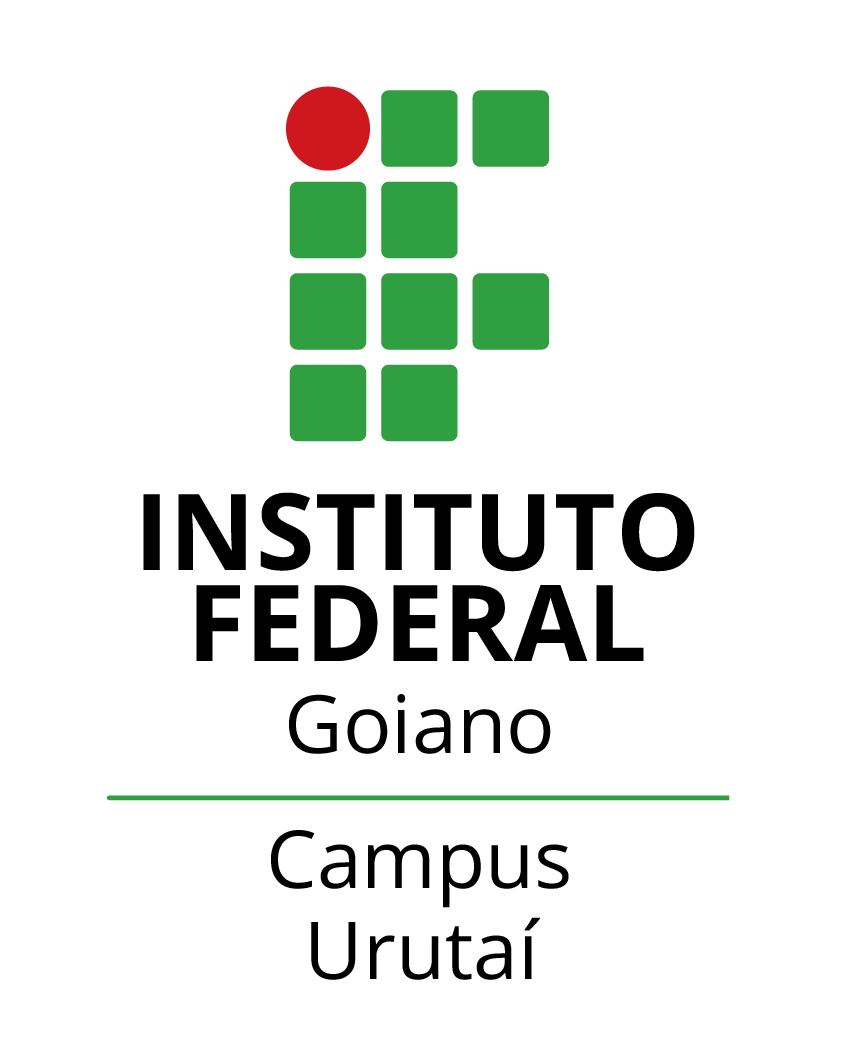
\includegraphics[scale=0.45]{figuras/logo_oficial.png} 
\bigskip
%---------------------------------------------
\hfill

%-------------SEGUNDA FIGURA(TEXTO)-----------
\begin{center}
\begin{large}
\textbf{\textsc{\instituicao}}\\
\textbf{\textsc\campus}\\
\small
\textsc{\unidade}\\
\textsc{Curso de \curso}\\
\medskip
\end{large}
\end{center}
%--------------------------------------------
\hfil

\end{center}

\vspace{1 cm}
\begin{Large}
\begin{center}
\textsc\autor\
\vspace{3cm}

\LARGE\textbf{\titulo}
\end{center}
\end{Large}

\vspace{3cm}
\vfill

\begin{center}
\local, \data
\end{center}



                   %inserindo a capa
%---------------------------------------------------------------------
\clearpage{\pagestyle{empty}\cleardoublepage %contracapa
\setcounter{page}{1}                         %começa a contar daqui
%\renewcommand{\thepage}{\roman{page}}        %o tipo de numeração    
\pagenumbering{arabic}
\pagestyle{empty}

%\thispagestyle{empty}
\thispagestyle{empty}
\begin{center}

\begin{minipage}[c]{0.8\linewidth}
\begin{large}
\begin{center}

\textbf{\textsc{\instituicao}}\\
\small
\textsc{\unidade}\\
\textsc{\curso}\\
\medskip

\end{center}
\end{large}
\end{minipage}
\end{center}

\vspace{1.8 cm}
\begin{Large}
\begin{center}
\textsc\autor\
\vspace{3cm}

\LARGE\textbf{\titulo}
\end{center}
\end{Large}

\vspace{3cm}
\vfill

\begin{center}
\begin{flushright}\begin{minipage}[b]{7.5cm}
{
\tipo\ apresentada ao \unidade, curso de \curso , do \instituicao, como parte das exigências para obtenção do título de \qualificacao\ em \area .
}
\end{minipage}\end{flushright}          \vskip 9em
{Orientador(a): \\ \orientador\par} \vfill


\vfill
{\local, \data }
\end{center}
         %inserindo a folha de rosto
\setcounter{page}{1}   
%-----------------------------------------------------------------
%INSERIR FICHA CATALOGRÁFICA
%		só depois que o trabalho estiver aprovado
%		para inserir basta adquirir a ficha catalografica
%		salvando-a em figuras, no formato pdf como nome de ficha.pdf
%		em seguida remova o simbolo de % das linhas a seguir



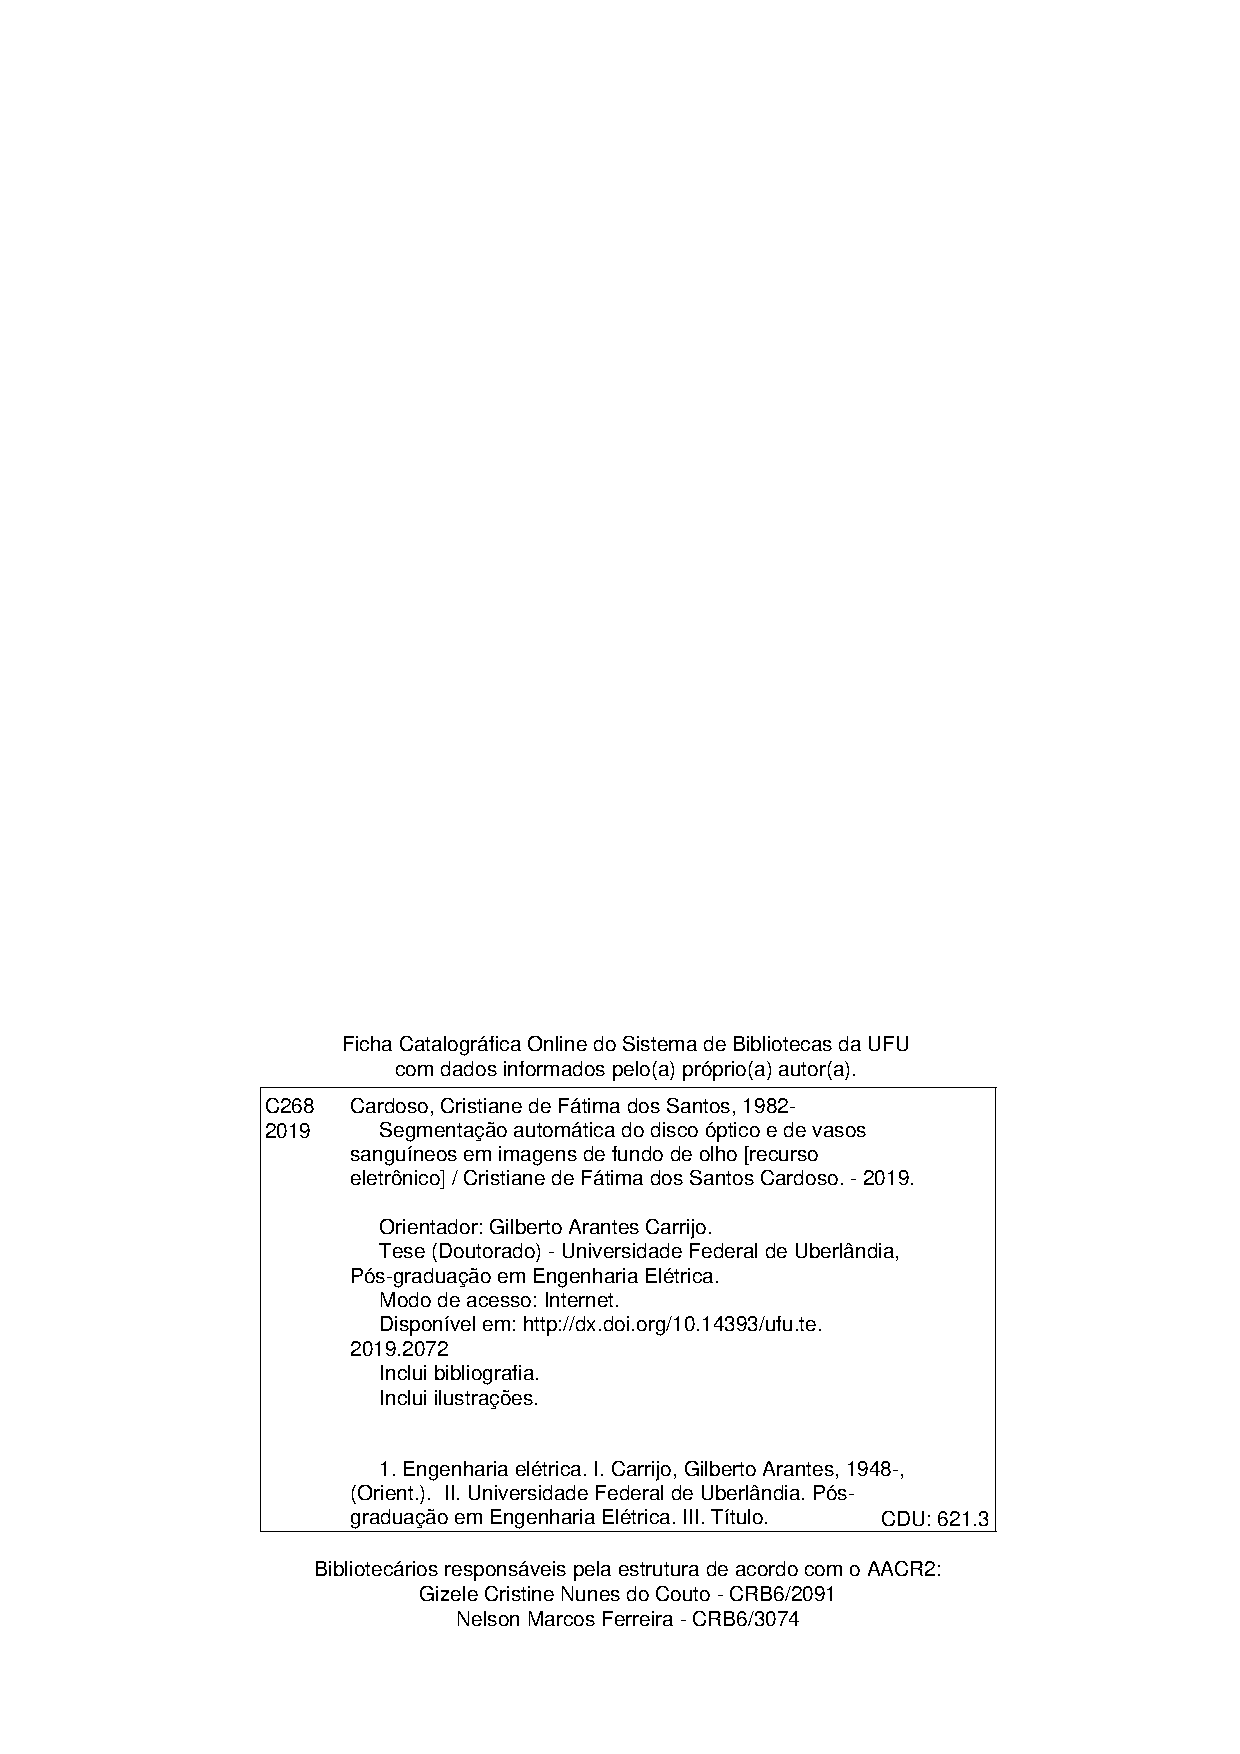
\includepdf{figuras/ficha.pdf}

   %ficha catalog.(SÓ NA VERSAO FINAL)
%\thispagestyle{empty}

\begin{center}
	\begin{LARGE}
		\sc\autor \par \vskip  4em
		\textbf{\titulo} \vskip  2em 
	\end{LARGE}	
\end{center}

\begin{flushleft}


\begin{minipage}{\linewidth}

\tipo\  defendida por \autor\ e aprovada em \datadefesa, pela banca examinadora constituída pelos membros: 

\end{minipage}
\end{flushleft}

\vspace{2cm}

\begin{center}


\rule{12cm}{0.01cm}

\titulacaoorientador\ \orientador  

\small{Orientador}\vfill


\rule{12cm}{0.01cm}

\titulacaoavaliadorum\ \avaliadorum 

\small{Avaliador}\vfill


\rule{12cm}{0.01cm}

\titulacaoavaliadordois\ \avaliadordois

\small{Avaliador}\vfill



\vspace{1cm}

\vfill


\local, \datadefesa 
\end{center}
\newpage     %folha de aprovação
% A dedicatória é um texto curto, não deve ultrapassar 5 linhas
% exemplo:

% 

\
\begin{dedicatoria}
\begin{large}
 \calligra{Dedico este trabalho aos meus ...}
\end{large}
\end{dedicatoria}          %dedicatoria - opcional
%\pagestyle{empty}
\begin{agradecimentos}

Agradeço a todos que contribuíram para a realização deste trabalho..


\end{agradecimentos}
       %agradecimentos-opcional
%%As chaves abaixo não devem ser retiradas
\epigrafe
{É uma citação relacionada ao assunto do texto}
{Autor da citação}
{Obra de onde foi retirada a citação}
             %epigrafe-opcional
%--------------------------------------------------------------------------
%		Não é necessário mudar qualquer coisa no preambulo deste arquivo
%		basta apenas colocar o seu texto, e as palavras-chave
%		observando as normas ABNT
%--------------------------------------------------------------------------
\chapter*{RESUMO} 
\thispagestyle{empty}
O resumo é um elemento obrigatório, e segundo a norma NBR6028:2003, ``Consiste na apresentação concisa do trabalho'', \cite[p.~1]{NBR6028:2003}. Deve descrever de forma clara e sintética a natureza do trabalho, o objetivo, o método, os resultados e as conclusões, visando fornecer elementos para o leitor decidir sobre a consulta do trabalho no todo. O resumo deve destacar: o assunto do trabalho; o objetivo do texto; as conclusões do trabalho. Deve ser redigido em linguagem clara e objetiva; ser inteligível por si mesmo (dispensar a consulta ao trabalho), evitar repetição de frases inteiras do trabalho, respeitar a ordem em que as ideias ou fatos são apresentados, empregar verbos na voz passiva, utilizar de preferência a 3ª pessoa do singular, evitar o uso de frases negativas, abreviaturas, fórmulas, quadros, equações, etc.
Para teses e dissertações, monografias, relatórios e TCCs o resumo deve ser
de 150 a 500 palavras. Deve ser redigido em parágrafo único, com frases completas,
sem sequência de itens/tópicos. Seguidas do resumo, as palavras-chave e descritores devem ser representativas ao conteúdo do trabalho, sendo as palavras-chave separadas entre si por ponto e finalizadas também por ponto. 
 
 
%--------------------------------------------------------------------------
\vspace{2cm}
{\Large \textbf{Palavras-chave:}}
\vspace{0.4cm}
%--------------------------------------------------------------------------

Latex. Modelos em latex. Monografia. 
%MAIS DICAS
%
%Passo 1: O que é (contexto)
%
%Para iniciar o resumo e abstract, apresente ao leitor do que se trata seu trabalho, ou seja, qual problema você está investigando e a sua relevância.
%
%Logo aqui, nas primeiras linhas, você precisa criar um contexto que desperte a curiosidade e o interesse para a leitura.
%
%Passo 2: Por quê? (Descreva o objetivo do trabalho)
%
%Com base no problema ou situação investigada, seu trabalho já precisa dizer a que veio. A forma de descrever um objetivo varia de acordo com o estudo realizado.
%
%Seu trabalho pode se propor a analisar diferentes aspectos de um mesmo problema, a compreender um fenômeno, ou então, a “apresentar uma solução para reduzir a produção de energia não renovável”, por exemplo. Em resumo, você conta o porquê do seu TCC existir.
%
%Passo 3: Como? (Método utilizado)
%
%Você deve explicar rapidamente como seu trabalho foi feito, qual metodologia utilizou. Conte ao seu leitor se você realizou um estudo de caso, um experimento, uma pesquisa quantitativa e/ou pesquisa qualitativa etc.
%
%Passo 4: Resultados
%
%Apresente os resultados mais relevantes do seu estudo, sejam eles positivos ou negativos. Descreva-os de forma sucinta, e que despertem curiosidade e interesse em quem lê.
%
%Passo 5: Conclui-se que…
%
%Por fim, seu resumo deve trazer as principais conclusões sobre tudo o que você leu, pesquisou e desenvolveu.
%
%Aqui, também é possível mencionar como o seu trabalho poderá contribuir para o entendimento do objeto ou fenômeno estudado, ou como servirá de base para pesquisas futuras.
%\vspace{-1cm}


               %resumo
%%--------------------------------------------------------------------------
%		Não é necessário mudar qualquer coisa no preambulo deste arquivo
%		basta apenas colocar o seu texto, e as palavras-chave
%		observando as normas ABNT
%--------------------------------------------------------------------------
\chapter*{ABSTRACT} 
\thispagestyle{empty}

The efficient segmentation of the optic disc and the blood vessels enables the development of an array of retinal images diagnostic tools, thus contributing for the medical diagnosis of pathologies such as Hypertensive and Diabetic retinopathy, Retinopathy of Prematurity, Glaucoma, retinal lesions caused by the Zika virus, etc. However, the step of segmentation of the optic disc and the blood vessels is considered by many one of the most difficult tasks in image processing, especially in colour fundus photography, which possesses lower contrast due to the prevalence of red in all the retina. Thus, the objective of this work is to segment the main physiological structures of the retina, those being the optic disc and the blood vessels. In order to do so, it was proposed (i) an algorithm based on a multiscale energy filter with a Hough transform to rapidly locate the disc and a decision criterion in the disc location, respectively; (ii) an algorithm based on 3D roughness index combined with mathematical morphology and the use of the Atanassov Intuitionistic Fuzzy Set representation to segment the optic disc; (iii) a multilayer perceptron neural network in which the differential is the setting of the pre-processing step based on Contrast Limited Adaptive Histogram Equalisation (CLAHE) and a Wiener filter to segment the blood vessels. As for results, it is observed that (i) the disc location method achieved 100\% effectiveness with the HRF and DRIVE databases, 98,5\% with the Messidor database and 94,38\% with the DIARETDB1 database; (ii) in the automatic segmentation of the optic disc with the Messidor database the accuracy achieved was of 99,59\% and the sensitivity was of 91,56\%; (iii) in the segmentation of the blood vessels, it is possible to fine-tune the pre-processing step allowing for a superior network performance; it was obtained an accuracy of 94,87\% for the first observer, and 95,31\% for the second observer in the DRIVE database, such figures exceed even more complex technologies.

%--------------------------------------------------------------------------
\vspace{2cm}
{\Large \textbf{Key-words:}}
\vspace{0.4cm}
%--------------------------------------------------------------------------


Fundus images. Digital Image Processing. RGB Segmentation. Energy filter. Hough Transform. A-IFS Histon. \textit{Roughness Index}. 

             %resumo

\clearpage{\pagestyle{empty}\cleardoublepage %verso do resumo em branco


%----------------------------------------------------------------
% INDICES E SUMÁRIO E GLOSSARIO
%	 	não é necessário editar. O latex faz tudo sozinho! 
%		IMPORTANTE: mudanças aparecem depois de Compilar/atualizar 
%		duas ou três vezes. NÃO SE ACANHE! SEJA INSISTENTE!
%		[no texmaker 3.5.2] ir em:
%		menu <Editar>-opção <Atualizar Estrutura>
%		Para adicionar
%%%%%%%%%%%%%%%%%%%%%%%%%%%%%%%%%%%%%%%%%%%%%%%%%%%%%%%%%%%%%%%%%%%
%		IMPORTANTE: para adicionar siglas use o comando 
%		\nomenclature{SIGLA}{DESCRIÇÃO} - em qualquer parte do texto
%		É necessário gerar a lista de acronimos, para isso, 
%		digite no terminal a seguinte linha de comando:
%
%		makeindex monografia.nlo -s nomencl.ist -o monografia.nls
%
%		no Texmaker, vá em <Ferramentas>-opção <Abrir Terminal>
%		e digite a referida linha
%
%	    Para adicionar entradas no glossário use o comando
%       \glossary{name={nome}, description={descrição}}
%       Exemplo: \glossary{name={ABNT}, description={Associação Brasileira de Normas Técnicas}}
%		A geração do glossário é parecida com a geração das siglas, digite no terminal: 
%
%       makeindex monografia.glo -s monografia.ist -t monografia.glg -o monografia.gls
%		
%%%%%%%%%%%%%%%%%%%%%%%%%%%%%%%%%%%%%%%%%%%%%%%%%%%%%%%%%%%%%%%%%%%
\pagestyle{plain}
%\clearpage{\pagestyle{empty}\cleardoublepage    %verso do resumo em branco
\renewcommand{\thepage}{\roman{page}}
\clearpage\listoffigures                        %lista de figuras - opcional
\newpage
\listoftables                        		    %lista de tabelas - opcional
\newpage
%\listofalgorithms                               %lista de algoritmos - opciona
\renewcommand{\nomname}{Lista de abreviaturas e siglas}     %renomeando lista de acronimos
\renewcommand{\pagedeclaration}{Pag.}            %renomeando lista de acronimos
% Siglas e abreviaturas usadas no texto. Cada \nomenclature gera uma entrada na
% "Lista de abreviaturas e siglas" (pacote nomencl); a ordem é alfabética.
\nomenclature{AED}{Análise Exploratória de Dados}
\nomenclature{ALT}{Alanina aminotransferase (TGP)}
\nomenclature{AST}{Aspartato aminotransferase (TGO)}
\nomenclature{AUC}{Área sob a curva (\textit{Area Under the Curve})}
\nomenclature{AUC-ROC}{Área sob a curva ROC}
\nomenclature{CSV}{Valores separados por vírgula (\textit{Comma-Separated Values})}
\nomenclature{CV}{Validação cruzada (\textit{cross-validation})}
\nomenclature{DP}{Desvio-padrão}
\nomenclature{F1}{Média harmônica entre precisão e sensibilidade}
\nomenclature{FN}{Falso negativo}
\nomenclature{FP}{Falso positivo}
\nomenclature{GOSS}{\textit{Gradient-based One-Side Sampling}}
\nomenclature{IC}{Intervalo de confiança}
\nomenclature{ILPD}{\textit{Indian Liver Patient Dataset}}
\nomenclature{IU}{Unidades internacionais (\textit{International Units})}
\nomenclature{KDD}{Descoberta de conhecimento em bases de dados (\textit{Knowledge Discovery in Databases})}
\nomenclature{LGB}{LightGBM (\textit{Light Gradient Boosting Machine})}
\nomenclature{OOB}{Fora da amostra \textit{bootstrap} (\textit{out-of-bag})}
\nomenclature{OR}{Razão de chances (\textit{odds ratio})}
\nomenclature{RF}{\textit{Random Forest}}
\nomenclature{RL}{Regressão Logística}
\nomenclature{ROC}{Característica de operação do receptor (\textit{Receiver Operating Characteristic})}
\nomenclature{SHAP}{\textit{SHapley Additive exPlanations}}
\nomenclature{SMOTE}{\textit{Synthetic Minority Over-sampling Technique}}
\nomenclature{SMOTE-NC}{SMOTE para variáveis nominais e contínuas (\textit{SMOTE-Nominal Continuous})}
\nomenclature{TGO}{Transaminase glutâmico-oxalacética (o mesmo que AST)}
\nomenclature{TGP}{Transaminase glutâmico-pirúvica (o mesmo que ALT)}
\nomenclature{UCI}{\textit{University of California, Irvine} (repositório de aprendizado de máquina)}
\nomenclature{VN}{Verdadeiro negativo}
\nomenclature{VP}{Verdadeiro positivo}
\nomenclature{XGB}{XGBoost (\textit{eXtreme Gradient Boosting})}
                   %siglas (entradas \nomenclature)
\printnomenclature	\label{listaacronimos}						    %gerando a lista de acronimos
\newpage
\chapter*{Lista de símbolos}
\addcontentsline{toc}{chapter}{Lista de símbolos}
\label{listasimbolos}

\begin{longtable}{@{}p{3.2cm}p{11.3cm}@{}}
\multicolumn{2}{@{}l}{\textit{Estatística e dados}} \\[0.2cm]
$n$ & Número de observações (pacientes) \\
$p$ & Número de variáveis preditoras \\
$x_i$, $y_i$ & Valor de uma variável na $i$-ésima observação \\
$\bar{x}$ & Média amostral da variável $x$ \\
$s$ & Desvio-padrão amostral (denominador $n-1$) \\
$x'$ & Valor transformado por $\ln(1 + x)$ (Equação~\ref{eq:log}) \\
$z$ & Valor padronizado (\textit{z-score}), $z = (x - \bar{x})/s$ \\
$b_1$ & Coeficiente de assimetria amostral \\
$r$ & Coeficiente de correlação de Pearson \\
$\ln$ & Logaritmo natural \\
$P(A \mid B)$ & Probabilidade de $A$ condicionada a $B$ \\
Valor-$p$ & Probabilidade associada ao resultado de um teste de hipótese \\[0.4cm]
\multicolumn{2}{@{}l}{\textit{Modelos de classificação}} \\[0.2cm]
$\mathbf{x}$ & Vetor de preditores de uma observação, $\mathbf{x} = (x_1, \ldots, x_p)$ \\
$Y$ & Variável-alvo ($Y = 1$ indica a classe positiva) \\
$\pi(\mathbf{x})$ & Probabilidade de a observação pertencer à classe positiva dado $\mathbf{x}$ \\
$\beta_0$, $\beta_j$ & Intercepto e coeficiente do preditor $x_j$ na Regressão Logística \\
$e^{\beta_j}$ & Razão de chances (\textit{odds ratio}) associada ao preditor $x_j$ \\
$B$ & Número de árvores do \textit{Random Forest} \\
$M$ & Número de iterações (árvores) do \textit{boosting} \\
$f_m$ & $m$-ésima árvore de regressão do \textit{boosting} \\
$F(\mathbf{x})$ & Escore aditivo do \textit{boosting} (escala do logaritmo da chance) \\
$\eta$ & Taxa de aprendizado \\
$\gamma$, $\lambda$ & Penalizações do número de folhas e da magnitude dos valores das folhas ($L_2$) no XGBoost \\[0.4cm]
\multicolumn{2}{@{}l}{\textit{Validação e métricas}} \\[0.2cm]
$k$ & Número de partições da validação cruzada e de vizinhos do SMOTE \\
VP, VN & Verdadeiros positivos e verdadeiros negativos \\
FP, FN & Falsos positivos e falsos negativos \\
AUC & Área sob a curva ROC \\[0.4cm]
\multicolumn{2}{@{}l}{\textit{Interpretabilidade (Shapley e SHAP)}} \\[0.2cm]
$\phi_j$ & Valor de Shapley (valor SHAP) da variável $j$ \\
$\phi_0$ & Valor base (saída média do modelo sobre o conjunto de referência) \\
$f(\mathbf{x})$ & Saída do modelo para a observação $\mathbf{x}$ \\
$n_{\mathrm{sim}}$ & Número de repetições da estimação por Monte Carlo \\
\end{longtable}                 %lista de símbolos
\newpage
\tableofcontents   							    %inserindo o sumário
\clearpage
%-----------------------------------------------------------------
% ELEMENTOS TEXTUAIS
%		localize cada um dos arquivos na pasta textuais
%       e edite da forma que desejar, caso necessite de 
% 		mais capitulos  é só criar os arquivos e incluir
%-----------------------------------------------------------------
\setlength{\baselineskip}{1.5\baselineskip}  %espaçamento entrelinhas 1.5
\pagestyle{fancy}							 %tipo de estilo da página - cabeçalho e rodapé
\renewcommand{\thepage}{\arabic{page}}
\citeoption{abnt-etal-cite=2}           % a partir de 2 autores, usa o et al.
\chapter{Fundamentação Teórica} \label{cap:fundamentacao}

Este capítulo apresenta os conceitos que fundamentam o trabalho, organizados segundo as etapas do processo de descoberta de conhecimento em bases de dados, a mesma sequência adotada na metodologia.

Inicialmente, descrevem-se esse processo e suas etapas (Seção~\ref{sec:fund_kdd}). Em seguida, são abordados os conceitos associados a cada etapa: a compreensão e a exploração dos dados, incluindo o domínio clínico do problema (Seção~\ref{sec:fund_estatistica}); a preparação dos dados (Seção~\ref{sec:fund_preparacao}); os modelos de classificação utilizados (Seção~\ref{sec:fund_modelos}); o treinamento, a validação e a avaliação dos modelos (Seção~\ref{sec:fund_validacao}); e a interpretação dos modelos (Seção~\ref{sec:fund_interpretabilidade}). Por fim, discute-se o viés algorítmico em saúde (Seção~\ref{sec:fund_vies}). Os termos básicos de estatística e aprendizado de máquina estão reunidos no Glossário (página~\pageref{glossario}), e os símbolos matemáticos, na Lista de Símbolos.

\section{Mineração de Dados e Descoberta de Conhecimento}
\label{sec:fund_kdd}

A descoberta de conhecimento em bases de dados (\textit{Knowledge Discovery in Databases}, KDD) é o processo de identificação de padrões válidos, novos e potencialmente úteis em conjuntos de dados \cite{Fayyad1996KDD}. A mineração de dados corresponde à etapa em que algoritmos extraem esses padrões; o resultado, entretanto, depende também da preparação dos dados que a antecede e da interpretação que a sucede, e o processo é iterativo \cite{Fayyad1996KDD}.

Neste trabalho, o processo foi organizado em cinco etapas (Figura~\ref{fig:fund_kdd}), cuja implementação computacional é denominada \textit{pipeline}. Na compreensão e exploração, caracterizam-se o problema e os dados; na preparação, os dados são tratados e transformados; na modelagem, os algoritmos são ajustados aos dados; no treinamento, validação e avaliação, estima-se o desempenho dos modelos; e, na interpretação, analisa-se de que forma os modelos produzem suas previsões. As setas tracejadas indicam que o processo não é linear, podendo um resultado de avaliação motivar a revisão de etapas anteriores. A ordem das operações foi definida de modo a evitar o vazamento de dados (Seção~\ref{sec:fund_vazamento}) \cite{KaufmanScharRosset2012, KAPOOR2023100804}.

Como diversas etapas envolvem procedimentos aleatórios, como a divisão entre treino e teste, a validação cruzada e o SMOTE, fixa-se a semente aleatória, isto é, o valor inicial do gerador de números pseudoaleatórios. A fixação da semente garante que os mesmos sorteios sejam reproduzidos em cada execução e, consequentemente, a reprodutibilidade dos resultados \cite{Pineau2020Improving}.

\begin{figure}[htbp]
\centering
\begin{tikzpicture}[
    etapa/.style={rectangle, rounded corners, draw, thick, align=center, text width=2.65cm, minimum height=1.8cm, font=\footnotesize\bfseries},
    itens/.style={rectangle, draw, align=left, text width=2.65cm, minimum height=2.7cm, font=\scriptsize, inner sep=3pt},
    seta/.style={->, thick, >=stealth}]
\node[etapa] (a) {1. Compreensão e exploração};
\node[etapa, right=0.3cm of a] (b) {2. Preparação dos dados};
\node[etapa, right=0.3cm of b] (c) {3. Modelagem};
\node[etapa, right=0.3cm of c] (d) {4. Treinamento, validação e avaliação};
\node[etapa, right=0.3cm of d] (e) {5. Interpretação dos modelos};
\node[itens, below=0.15cm of a, anchor=north] {\textbullet~Caracterização e qualidade da base\\ \textbullet~Estatísticas e assimetria\\ \textbullet~Comparação entre classes\\ \textbullet~Correlação};
\node[itens, below=0.15cm of b, anchor=north] {\textbullet~Remoção de duplicatas\\ \textbullet~Transformação logarítmica\\ \textbullet~Divisão treino/teste\\ \textbullet~Imputação\\ \textbullet~Padronização\\ \textbullet~SMOTE (só no treino)};
\node[itens, below=0.15cm of c, anchor=north] {\textbullet~Regressão Logística\\ \textbullet~\textit{Random Forest}\\ \textbullet~XGBoost\\ \textbullet~LightGBM};
\node[itens, below=0.15cm of d, anchor=north] {\textbullet~Validação cruzada repetida\\ \textbullet~Busca aleatória de hiperparâmetros\\ \textbullet~Seleção pela AUC-ROC\\ \textbullet~Avaliação no teste e limiares\\ \textbullet~Comparação entre modelos};
\node[itens, below=0.15cm of e, anchor=north] {\textbullet~SHAP (TreeSHAP e Monte Carlo)\\ \textbullet~Importância global e local\\ \textbullet~Auditoria por sexo\\ \textbullet~Comparação de rankings};
\draw[seta] (a) -- (b);
\draw[seta] (b) -- (c);
\draw[seta] (c) -- (d);
\draw[seta] (d) -- (e);
\draw[seta, dashed] (d.north) -- ++(0,0.6) -| node[pos=0.25, above, font=\footnotesize] {retorno às etapas anteriores, quando necessário} (a.north);
\end{tikzpicture}

\caption{Fluxo (\textit{pipeline}) adotado neste trabalho, organizado nas etapas do processo de descoberta de conhecimento.}
\label{fig:fund_kdd}
{\small Fonte: elaborado pelo autor, com base em \citeonline{Fayyad1996KDD}.}
\end{figure}

A Tabela~\ref{tab:fund_kdd} apresenta a correspondência entre cada etapa do processo e os procedimentos realizados neste trabalho, detalhados no Capítulo~\ref{metodologia}.

\begin{table}[htbp]
\centering
\begin{tabular}{>{\raggedright\arraybackslash}p{4.2cm}>{\raggedright\arraybackslash}p{9.8cm}}
\hline
\textbf{Etapa} & \textbf{Procedimentos realizados} \\
\hline
Compreensão e exploração dos dados & Escolha da base ILPD; verificação de qualidade, valores ausentes e duplicatas; estatísticas descritivas, assimetria, comparação entre doentes e saudáveis e correlação entre os exames. \\[0.1cm]
Preparação dos dados & Remoção de duplicatas; transformação logarítmica dos exames assimétricos; divisão em treino e teste; imputação pela mediana; padronização; balanceamento com SMOTE apenas no treino. \\[0.1cm]
Modelagem & Treinamento da Regressão Logística, do \textit{Random Forest}, do XGBoost e do LightGBM. \\[0.1cm]
Treinamento, validação e avaliação & Validação cruzada repetida; busca aleatória de hiperparâmetros; avaliação no conjunto de teste com matriz de confusão, AUC e teste de DeLong; limiar clínico; avaliação por sexo. \\[0.1cm]
Interpretação dos modelos & Valores SHAP: importância das variáveis, sentido e forma dos efeitos, explicação de pacientes individuais, auditoria por sexo e comparação entre modelos. \\
\hline
\end{tabular}
\caption{Correspondência entre as etapas do processo de descoberta de conhecimento e os procedimentos deste trabalho.}
\label{tab:fund_kdd}
\par\vspace{2pt}{\small Fonte: elaborado pelo autor.}
\end{table}

\section{Compreensão e Exploração dos Dados}
\label{sec:fund_estatistica}

A Análise Exploratória de Dados (AED) reúne resumos numéricos e representações gráficas empregados para caracterizar a estrutura e a qualidade das variáveis antes da modelagem \cite{exploratorydataanalysis}. Nessa etapa, identificam-se valores ausentes, registros duplicados, valores extremos e variáveis redundantes, achados que orientam as decisões de preparação dos dados. A AED tem caráter exclusivamente descritivo: nenhuma estatística nela calculada deve ser utilizada para transformar os dados empregados no ajuste dos modelos (Seção~\ref{sec:fund_vazamento}).

\subsection{Domínio do Problema: Doença Hepática e Marcadores Laboratoriais}
\label{sec:fund_figado}

O fígado é responsável pela síntese da maior parte das proteínas plasmáticas, como a albumina, e pela eliminação da bilirrubina, pigmento resultante da degradação da hemoglobina. Doença hepática é o termo geral que designa as condições que lesam o fígado ou comprometem seu funcionamento, como as hepatites e a cirrose. Sua investigação inicial recorre a exames laboratoriais, cujos valores podem atingir várias vezes o limite superior da faixa de referência \cite{Giannini2005Liver, Kwo2016ACG}.

Cada marcador reflete um aspecto da função hepática. A alanina aminotransferase (ALT) e a aspartato aminotransferase (AST) são enzimas intracelulares liberadas na circulação quando há lesão dos hepatócitos e, por isso, tendem a elevar-se conjuntamente \cite{Kwo2016ACG, Newsome2018Guidelines}. A fosfatase alcalina eleva-se na obstrução do fluxo biliar, e a bilirrubina, em ambas as situações; a bilirrubina direta corresponde à fração conjugada pelo fígado e integra a bilirrubina total \cite{Kwo2016ACG}. As proteínas totais, a albumina e a razão albumina/globulina refletem a capacidade de síntese proteica, e a redução da albumina indica comprometimento dessa função \cite{Busher1990Albumin}. Em consequência, diversos exames carregam informação parcialmente redundante e são correlacionados, e suas distribuições são assimétricas, com valores extremos que decorrem da própria doença, e não necessariamente de erros de medição.

\subsection{Conceitos Básicos de Dados e Aprendizado Supervisionado}
\label{sec:fund_conceitos}

Em uma base de dados tabular, cada linha corresponde a uma observação, neste trabalho um paciente, e cada coluna, a uma variável. As variáveis podem ser numéricas, como os exames laboratoriais, ou categóricas, como o sexo. No aprendizado supervisionado, uma das variáveis é a variável-alvo, que se deseja prever, e as demais são os preditores; quando a variável-alvo é categórica, a tarefa é denominada classificação \cite{elementsofstatiscal}. O modelo é ajustado em um conjunto de treino e avaliado em um conjunto de teste, independente, que representa observações não vistas durante o ajuste \cite{elementsofstatiscal}.

Em problemas com duas classes, denomina-se positiva a classe que se deseja detectar, neste trabalho ``doente'', e negativa a outra, ``saudável''. A base é dita desbalanceada quando uma das classes, a majoritária, possui número de observações substancialmente maior que a outra, a minoritária. A proporção de observações de uma classe é denominada prevalência.

\subsection{Estatísticas Descritivas e Assimetria}
\label{sec:fund_assimetria}

As estatísticas descritivas resumem a distribuição de uma variável. A média é sensível a valores extremos (\textit{outliers}), ao passo que a mediana é pouco afetada por eles \cite{han2012getting}; assim, uma média consideravelmente superior à mediana indica a presença de uma cauda de valores elevados, isto é, de assimetria positiva.

O coeficiente de assimetria (\textit{skewness}) quantifica esse comportamento: assume valores próximos de zero em distribuições simétricas e valores positivos quando poucos valores muito elevados formam uma cauda à direita, situação frequente em exames laboratoriais. A assimetria acentuada distorce estatísticas como a média e o coeficiente de correlação de Pearson e confere peso excessivo a poucas observações em modelos lineares, como a Regressão Logística. Não há um limite universal para caracterizar a assimetria como excessiva; \citeonline[p.~26]{curran1996robustness} identificaram problemas a partir de 2,0, valor adotado neste trabalho como convenção. No contexto da doença hepática, valores extremos podem constituir o próprio fenômeno de interesse e, portanto, não devem ser descartados \cite[p.~237]{Aggarwal2015}.

\subsection{Correlação e Multicolinearidade}
\label{sec:fund_correlacao}

O coeficiente de correlação de Pearson ($r$) mede o grau de associação linear entre duas variáveis e varia de $-1$ a $+1$; valores próximos de zero indicam ausência de associação linear, e valores absolutos superiores a 0,7 costumam indicar correlação forte \cite{Dormann2013Collinearity}. O coeficiente de correlação de Spearman é calculado sobre os postos, isto é, sobre as posições dos valores ordenados, e é menos sensível a valores extremos \cite{Schober2018Correlation}.

Quando preditores são fortemente correlacionados entre si, ocorre multicolinearidade: as variáveis carregam informação semelhante, o que afeta principalmente a interpretação dos modelos, e não sua capacidade preditiva \cite{Strobl2008Conditional, Dormann2013Collinearity}. É o que ocorre com as bilirrubinas total e direta, cuja variação conjunta impede que o modelo atribua a cada uma, isoladamente, sua contribuição para a previsão.

\subsection{Testes de Hipótese e Comparações Múltiplas}
\label{sec:fund_bonferroni}

Um teste de hipótese avalia se os dados fornecem evidência contra uma hipótese nula, que em geral estabelece a ausência de diferença ou de efeito. O valor-$p$ corresponde à probabilidade de se observar um resultado ao menos tão extremo quanto o obtido, supondo verdadeira a hipótese nula. Rejeita-se a hipótese nula quando o valor-$p$ é inferior ao nível de significância adotado, convencionalmente 0,05. Neste trabalho, testes de hipótese são empregados na avaliação dos coeficientes da Regressão Logística e na comparação do desempenho dos modelos.

Quando diversos testes são realizados sobre os mesmos dados, aumenta a probabilidade de que algum resultado seja considerado significativo apenas por acaso. A correção de Bonferroni controla esse efeito multiplicando cada valor-$p$ pelo número de comparações realizadas, com limite superior igual a 1 \cite{Demsar2006Statistical}. Trata-se de uma correção conservadora, que reduz a ocorrência de falsos positivos à custa de menor capacidade de detectar diferenças reais.

\section{Preparação dos Dados}
\label{sec:fund_preparacao}

A preparação dos dados converte os dados brutos em uma representação adequada aos algoritmos e pode influenciar o resultado tanto quanto a escolha do modelo \cite{KAPOOR2023100804}. Ela compreende o tratamento de valores ausentes e de registros duplicados, a transformação da escala das variáveis e o balanceamento das classes, sempre de modo a impedir que informação do conjunto de teste seja utilizada no treinamento.

\subsection{Valores Ausentes, Registros Duplicados e Vazamento de Dados}
\label{sec:fund_ausentes}
\label{sec:fund_vazamento}

Valores ausentes correspondem a informações não registradas para algumas observações. Em vez da exclusão das observações afetadas, pode-se recorrer à imputação, que substitui cada valor ausente por uma estimativa; a mediana é preferível à média por ser robusta aos valores extremos característicos dos exames laboratoriais \cite{batistamonard2003}. Registros duplicados, por sua vez, são observações idênticas em todas as variáveis.

Ambos os casos relacionam-se ao vazamento de dados (\textit{data leakage}), que ocorre quando informação do conjunto de teste é incorporada, direta ou indiretamente, ao treinamento, o que torna a estimativa de desempenho excessivamente otimista \cite{KaufmanScharRosset2012, KAPOOR2023100804}. O vazamento pode decorrer da presença de um registro no treino e de sua duplicata no teste, do cálculo de parâmetros de transformação, como a mediana da imputação ou a média da padronização, a partir de todos os dados, ou do balanceamento das classes antes da divisão (Seção~\ref{sec:fund_smote}). Por esse motivo, tais operações devem ser ajustadas exclusivamente no conjunto de treino e, em seguida, aplicadas ao conjunto de teste.

\subsection{Transformação Logarítmica e Padronização}
\label{sec:fund_log}
\label{sec:fund_padronizacao}

Variáveis com distribuição de cauda longa, como os exames hepáticos, podem ter sua assimetria reduzida por meio da transformação logarítmica \cite{logtransformation}:
\begin{equation}
    x' = \ln(1 + x),
    \label{eq:log}
\end{equation}
em que $x$ é o valor original e $x'$, o valor transformado. A transformação comprime proporcionalmente mais os valores elevados do que os reduzidos, preservando a ordem entre as observações. No ILPD, a AST apresenta mediana de 42~IU/L e máximo de 4.929~IU/L; após a transformação, esses valores passam a 3,76 e 8,50, respectivamente. A adição de uma unidade evita a indefinição do logaritmo para valores nulos. Como a transformação nem sempre reduz a assimetria, seu efeito deve ser verificado pelo recálculo do coeficiente de assimetria \cite{logtransformation}. Por depender apenas do valor de cada observação, e não de parâmetros estimados a partir dos dados, a transformação pode ser aplicada antes da divisão entre treino e teste sem ocasionar vazamento.

A padronização (\textit{z-score}), definida por $z = (x - \bar{x})/s$, expressa cada valor em número de desvios-padrão em relação à média, de modo que todas as variáveis passam a ter média zero e desvio-padrão unitário. Como a média $\bar{x}$ e o desvio-padrão $s$ são estimados a partir dos dados, devem ser calculados apenas no conjunto de treino e, posteriormente, aplicados ao conjunto de teste.

Ambas as operações são relevantes principalmente para a Regressão Logística: a padronização torna os coeficientes comparáveis entre si, pois cada um passa a expressar o efeito de um desvio-padrão \cite{Hosmer2005Applied}, e a transformação logarítmica reduz a influência das observações extremas sobre o ajuste. Para os modelos baseados em árvores de decisão, o efeito é reduzido, uma vez que as divisões dependem apenas da ordem dos valores, preservada por transformações monotônicas \cite{elementsofstatiscal}.

\subsection{Desbalanceamento de Classes e SMOTE}
\label{sec:fund_smote}

Em bases desbalanceadas, um classificador pode obter acurácia elevada prevendo sempre a classe majoritária \cite{FAWCETT2006861}. No ILPD, em que 71\% dos pacientes pertencem à classe ``doente'', esse classificador trivial apresentaria acurácia de 71\% sem identificar nenhum paciente saudável.

O SMOTE (\textit{Synthetic Minority Over-sampling Technique}) \cite{smote} é uma técnica de sobreamostragem que gera observações sintéticas da classe minoritária. Para cada observação dessa classe, seleciona-se aleatoriamente um de seus $k$ vizinhos mais próximos da mesma classe, e a nova observação é gerada em um ponto sorteado do segmento que une as duas. Em variáveis binárias, como o sexo, essa interpolação produz valores sem significado, limitação tratada pela variante SMOTE-NC \cite{smote}.

A reamostragem deve ser aplicada exclusivamente ao conjunto de treino e, quando há validação cruzada, dentro de cada partição de treino, a fim de evitar vazamento \cite{KaufmanScharRosset2012}. Além disso, ao alterar a proporção de classes apresentada ao modelo, o SMOTE faz com que as probabilidades previstas deixem de refletir a prevalência real \cite{vandenGoorbergh2022Harm}, tendendo, neste caso, a subestimar a probabilidade de doença.

\section{Modelagem e Classificação}
\label{sec:fund_modelos}

Um modelo de classificação recebe os preditores de uma observação e estima a probabilidade de que ela pertença à classe positiva. O principal risco do treinamento é o sobreajuste (\textit{overfitting}), situação em que o modelo se ajusta a particularidades e ruídos do conjunto de treino e apresenta baixa capacidade de generalização para novas observações.

Neste trabalho, foram empregados quatro modelos: a Regressão Logística e três métodos de \textit{ensemble} baseados em árvores de decisão. A inclusão da Regressão Logística como referência fundamenta-se na revisão sistemática de \citeonline{Christodoulou2019Systematic}, que, ao analisar 71 estudos de predição clínica, não identificou vantagem dos métodos de aprendizado de máquina sobre a regressão logística nas comparações com baixo risco de viés.

\subsection{Regressão Logística}
\label{sec:fund_lr}

A Regressão Logística \cite{Cox1958Regression} modela o logaritmo da chance (\textit{odds}), definida como a razão entre a probabilidade de ocorrência do evento e a de sua não ocorrência, como uma combinação linear dos preditores \cite{Hosmer2005Applied}:
\begin{equation}
    \ln\left(\frac{\pi(\mathbf{x})}{1 - \pi(\mathbf{x})}\right) = \beta_0 + \sum_{j=1}^{p} \beta_j x_j,
    \label{eq:logit}
\end{equation}
em que $\pi(\mathbf{x})$ é a probabilidade de doença, $\beta_0$ é o intercepto e $\beta_j$ é o coeficiente associado ao preditor $x_j$. A significância de cada coeficiente é avaliada pelo teste de Wald.

A principal vantagem do modelo é a interpretação direta de seus coeficientes: mantidos constantes os demais preditores, o aumento de uma unidade em $x_j$ multiplica a chance de doença pela razão de chances $e^{\beta_j}$ \cite{Hosmer2005Applied}. Essa interpretação torna-se pouco confiável na presença de preditores fortemente correlacionados, cujos coeficientes são instáveis e podem inclusive apresentar sinal oposto ao esperado \cite{Dormann2013Collinearity}.

\subsection{Árvores de Decisão e Métodos de \textit{Ensemble}}
\label{sec:fund_arvores}

Uma árvore de decisão classifica uma observação por meio de uma sequência de regras sobre as variáveis, organizadas hierarquicamente, até alcançar um nó terminal, denominado folha, que indica a classe prevista \cite{elementsofstatiscal}. A Figura~\ref{fig:fund_arvore} apresenta um exemplo ilustrativo. Árvores individuais são de fácil interpretação, mas instáveis: pequenas alterações no conjunto de treino podem produzir árvores substancialmente diferentes.

Os métodos de \textit{ensemble} combinam múltiplas árvores para reduzir essa instabilidade. No \textit{bagging}, as árvores são treinadas de forma independente, cada uma em uma amostra distinta dos dados, e suas previsões são combinadas por votação. No \textit{boosting}, as árvores são treinadas sequencialmente, cada uma buscando corrigir os erros das anteriores. Em contrapartida, o modelo resultante perde a interpretabilidade direta e passa a ser considerado um modelo de caixa-preta.

\begin{figure}[htbp]
\centering
\begin{tikzpicture}[
    perg/.style={rectangle, rounded corners, draw, thick, align=center, font=\footnotesize, inner sep=4pt},
    folha/.style={rectangle, draw, fill=gray!20, align=center, font=\footnotesize, inner sep=4pt},
    level distance=1.6cm, sibling distance=5.2cm, edge from parent/.style={draw, -{Stealth}, thick}]
\node[perg] {Bilirrubina total $> 1{,}8$~mg/dL?}
  child {node[folha] {Doente}
    edge from parent node[left, font=\scriptsize, xshift=-3pt] {sim}}
  child {node[perg] {AST $> 60$~IU/L?}
    child {node[folha] {Doente} edge from parent node[left, font=\scriptsize, xshift=-3pt] {sim}}
    child {node[folha] {Saudável} edge from parent node[right, font=\scriptsize, xshift=3pt] {não}}
    edge from parent node[right, font=\scriptsize, xshift=3pt] {não}};
\end{tikzpicture}
\caption{Exemplo ilustrativo de árvore de decisão com dois exames do ILPD. Os pontos de corte são apenas ilustrativos.}
\label{fig:fund_arvore}
{\small Fonte: elaborado pelo autor.}
\end{figure}

\subsection{\textit{Random Forest}}
\label{sec:fund_rf}

O \textit{Random Forest} \cite{Breiman2001RandomForests} aplica o \textit{bagging} a árvores de decisão. Cada árvore é treinada em uma amostra \textit{bootstrap}, obtida por sorteio com reposição a partir do conjunto de treino, e, em cada divisão, apenas um subconjunto aleatório de \texttt{mtry} variáveis é considerado, o que aumenta a diversidade entre as árvores. A probabilidade estimada de doença corresponde à fração de árvores que atribuem a observação a essa classe. O aumento do número de árvores não provoca sobreajuste, e o método tende a apresentar bom desempenho com os valores padrão de seus hiperparâmetros \cite{Breiman2001RandomForests, Probst2019Hyperparameters}.

\subsection{XGBoost}
\label{sec:fund_xgb}

O XGBoost \cite{Chen2016XGBoost} é uma implementação regularizada do \textit{gradient boosting} \cite{Friedman2001Greedy}, método em que cada nova árvore é ajustada aos resíduos das previsões acumuladas até a iteração anterior. A previsão final é a soma das contribuições de todas as árvores, convertida em probabilidade pela função logística:
\begin{equation}
    F(\mathbf{x}) = \sum_{m=1}^{M} f_m(\mathbf{x}),
    \qquad
    \hat{\pi}(\mathbf{x}) = \frac{1}{1 + e^{-F(\mathbf{x})}},
    \label{eq:boosting}
\end{equation}
em que $f_m$ é a $m$-ésima árvore, $M$ é o número de iterações e $F(\mathbf{x})$ é expresso na escala do logaritmo da chance.

Para controlar o sobreajuste, a taxa de aprendizado $\eta$ reduz a contribuição de cada árvore, e os termos de regularização $\gamma$ e $\lambda$ penalizam, respectivamente, o número de folhas e a magnitude dos valores atribuídos a elas \cite{Chen2016XGBoost}. Em dados tabulares, o XGBoost figura entre os métodos de melhor desempenho \cite{Grinsztajn2022Why}.

\subsection{LightGBM}
\label{sec:fund_lgbm}

O LightGBM \cite{Ke2017LightGBM} baseia-se no mesmo princípio de \textit{boosting} (Equação~\ref{eq:boosting}), com ênfase na eficiência computacional. O algoritmo discretiza os valores contínuos em intervalos e expande cada árvore a partir da folha que proporciona maior redução do erro (\textit{leaf-wise}), em vez de expandi-la nível a nível. Em bases pequenas, essa estratégia pode favorecer o sobreajuste, razão pela qual se recomenda limitar o número de folhas e estabelecer um número mínimo de observações por folha \cite{LightGBMDocsTuning}.

\section{Treinamento, Validação e Avaliação}
\label{sec:fund_validacao}

Além do ajuste aos dados de treino, é necessário estimar o desempenho do modelo em observações não utilizadas no treinamento, isto é, sua capacidade de generalização. Esta seção trata da estimação do desempenho sem o uso do conjunto de teste, da escolha das configurações dos algoritmos, das métricas de avaliação e da definição do limiar de decisão.

\subsection{Validação Cruzada}
\label{sec:fund_cv}

Na validação cruzada $k$-\textit{fold}, o conjunto de treino é dividido em $k$ partes de tamanhos semelhantes, denominadas \textit{folds}. O modelo é treinado com $k-1$ partes e avaliado na parte restante, procedimento repetido até que cada parte tenha sido utilizada uma vez para avaliação (Figura~\ref{fig:fund_cv}). O desempenho estimado corresponde à média das $k$ avaliações \cite{elementsofstatiscal}.

\begin{figure}[htbp]
\centering
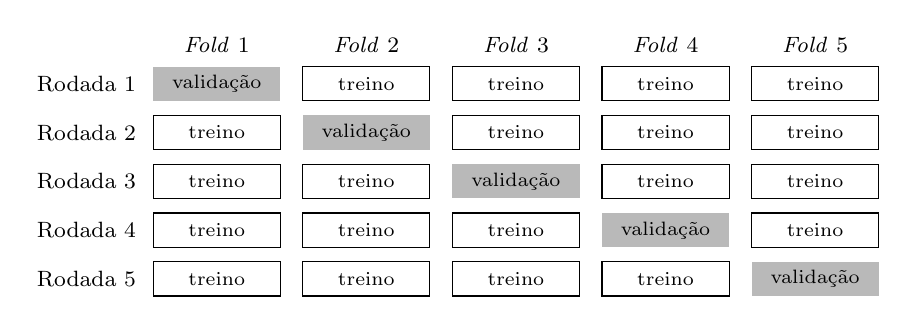
\begin{tikzpicture}[x=1.9cm, y=0.62cm]
\foreach \lin in {1,...,5} {
  \node[anchor=east, font=\footnotesize] at (0.05,-\lin) {Rodada \lin};
  \foreach \col in {1,...,5} {
    \ifnum\col=\lin
      \fill[gray!55] (\col-1+0.1,-\lin-0.35) rectangle (\col-0.05,-\lin+0.35);
      \node[font=\scriptsize] at (\col-0.475,-\lin) {validação};
    \else
      \draw (\col-1+0.1,-\lin-0.35) rectangle (\col-0.05,-\lin+0.35);
      \node[font=\scriptsize] at (\col-0.475,-\lin) {treino};
    \fi
  }
}
\foreach \col in {1,...,5} { \node[font=\footnotesize] at (\col-0.475,-0.2) {\textit{Fold} \col}; }
\end{tikzpicture}
\caption{Validação cruzada com $k = 5$: em cada rodada, uma parte diferente do conjunto de treino é usada para avaliar o modelo treinado com as outras quatro.}
\label{fig:fund_cv}
{\small Fonte: elaborado pelo autor.}
\end{figure}

As previsões obtidas para as observações da parte reservada, produzidas por um modelo que não as utilizou no ajuste, são denominadas previsões fora da partição (\textit{out-of-fold}). Ao final das $k$ rodadas, cada observação do treino dispõe de uma previsão desse tipo, o que permite, entre outras aplicações, a escolha do limiar de decisão sem o uso do conjunto de teste (Seção~\ref{sec:fund_limiar}). A estratificação preserva, em cada parte, a proporção de classes da base. Os valores mais utilizados de $k$ são 5 e 10, que representam um compromisso entre o viés e a variância da estimativa \cite{elementsofstatiscal}. Como o resultado depende da alocação das observações entre as partes, o procedimento pode ser repetido com diferentes sorteios, o que reduz a variabilidade da estimativa \cite{Kim2009Estimating}.

\subsection{Hiperparâmetros e Sua Otimização}
\label{sec:fund_hiperparametros}

Os parâmetros de um modelo são estimados a partir dos dados durante o treinamento, como os coeficientes da Regressão Logística. Os hiperparâmetros, por sua vez, são definidos antes do treinamento e controlam o processo de aprendizado, como o número de variáveis consideradas em cada divisão do \textit{Random Forest}, a profundidade máxima das árvores e a taxa de aprendizado do XGBoost.

A otimização de hiperparâmetros consiste em avaliar diferentes combinações, em geral por validação cruzada, e selecionar a de melhor desempenho. Na busca em grade, avaliam-se todas as combinações de um conjunto predefinido de valores, cujo número cresce exponencialmente com a quantidade de hiperparâmetros. Na busca aleatória, avalia-se um número fixo de combinações sorteadas, estratégia que tende a obter resultados comparáveis aos da busca em grade com custo computacional muito inferior \cite{Bergstra2012Random}. Como a combinação selecionada é justamente a de melhor desempenho na validação cruzada, a estimativa obtida nessa etapa tende a ser otimista \cite{Cawley2010OverFitting}; por isso, o desempenho final deve ser estimado em um conjunto de teste que não tenha participado da seleção.

\subsection{Métricas de Desempenho}
\label{sec:fund_metricas}
\label{sec:fund_matriz}

Os modelos utilizados neste trabalho estimam a probabilidade de doença. A classe prevista é obtida pela comparação dessa probabilidade com um limiar de decisão, de modo que observações com probabilidade igual ou superior ao limiar são classificadas como positivas. A matriz de confusão (Tabela~\ref{tab:matriz_confusao}) cruza as classes previstas com as classes reais e define quatro resultados: verdadeiros positivos (VP), falsos negativos (FN), verdadeiros negativos (VN) e falsos positivos (FP) \cite{FAWCETT2006861}.

\begin{table}[htbp]
\centering
\begin{tabular}{llcc}
\hline
 & & \multicolumn{2}{c}{\textbf{Classe real}} \\
 & & \textbf{Doente} & \textbf{Saudável} \\
\hline
\multirow{2}{*}{\textbf{Classe prevista}} & \textbf{Doente} & VP & FP \\
 & \textbf{Saudável} & FN & VN \\
\hline
\end{tabular}
\caption{Matriz de confusão, com ``doente'' como classe positiva.}
\label{tab:matriz_confusao}
\end{table}

A partir da matriz de confusão, definem-se as seguintes métricas \cite{FAWCETT2006861}:

\begin{itemize}
    \item \textit{acurácia}: proporção de classificações corretas, $(\mathrm{VP} + \mathrm{VN}) / (\mathrm{VP} + \mathrm{FP} + \mathrm{FN} + \mathrm{VN})$;
    \item \textit{sensibilidade}: proporção de doentes corretamente identificados, $\mathrm{VP} / (\mathrm{VP} + \mathrm{FN})$;
    \item \textit{especificidade}: proporção de saudáveis corretamente identificados, $\mathrm{VN} / (\mathrm{VN} + \mathrm{FP})$;
    \item \textit{precisão}: proporção de doentes entre as observações classificadas como doentes, $\mathrm{VP} / (\mathrm{VP} + \mathrm{FP})$.
\end{itemize}

Em bases desbalanceadas, a acurácia isolada é inadequada, pois pode ser elevada mesmo para um classificador sem capacidade de discriminação \cite{FAWCETT2006861}; por essa razão, deve ser acompanhada da sensibilidade e da especificidade. A precisão, diferentemente das demais, depende da prevalência da classe positiva no grupo avaliado e, por isso, não é adequada para comparar grupos com prevalências distintas (Seção~\ref{sec:fund_vies}).

\subsection{Curva ROC, AUC e Teste de DeLong}
\label{sec:fund_roc}
\label{sec:fund_delong}

As métricas apresentadas dependem do limiar adotado: a redução do limiar aumenta a sensibilidade e diminui a especificidade, e vice-versa. A curva ROC (\textit{Receiver Operating Characteristic}) representa essa relação para todos os limiares possíveis, com a taxa de falsos positivos ($1 -$ especificidade) no eixo horizontal e a sensibilidade no eixo vertical. Modelos com boa capacidade de discriminação apresentam curvas próximas ao canto superior esquerdo do gráfico, enquanto um classificador aleatório corresponde à diagonal.

A área sob a curva ROC (AUC-ROC) corresponde à probabilidade de que, dado um par formado por uma observação positiva e uma negativa sorteadas ao acaso, o modelo atribua maior probabilidade à observação positiva \cite{FAWCETT2006861, Hanley1982Meaning}. A AUC-ROC assume o valor 0,5 para um classificador aleatório e 1 para uma separação perfeita. Por independer do limiar e da proporção entre as classes, permite comparar modelos antes da definição do limiar de decisão.

Por ser estimada a partir de uma amostra, a AUC-ROC está sujeita a incerteza, expressa por meio de um intervalo de confiança, cuja amplitude aumenta à medida que o tamanho da amostra diminui. O método de DeLong \cite{DeLong1988Comparing} permite calcular esse intervalo e testar a diferença entre as AUC-ROC de dois modelos avaliados nas mesmas observações, considerando a correlação entre as estimativas decorrente do pareamento \cite{DeLong1988Comparing, Robin2011pROC}.

\subsection{Limiar de Decisão}
\label{sec:fund_limiar}

O limiar de 0,5 minimiza o custo esperado dos erros apenas quando as probabilidades previstas são bem calibradas, isto é, correspondem às frequências observadas, e quando os dois tipos de erro têm o mesmo custo \cite{Elkan2001Foundations}. Na triagem clínica, avaliação inicial destinada a identificar os pacientes que necessitam de investigação adicional, os custos são assimétricos: o falso negativo pode atrasar o diagnóstico, enquanto o falso positivo tende a resultar apenas em exames complementares \cite{Habibzadeh2016Determining}. Nesse contexto, justifica-se a adoção de limiares inferiores a 0,5, que aumentam a sensibilidade à custa da especificidade.

Uma estratégia para priorizar a sensibilidade consiste em fixar uma meta mínima, como 90\%, e selecionar o maior limiar que a satisfaz, preservando a maior especificidade possível. Essa escolha deve ser realizada em dados distintos daqueles utilizados na avaliação, pois o ajuste do limiar nas próprias previsões do conjunto de teste produziria estimativas otimistas \cite{Leeflang2008Bias}. A escolha a partir das previsões fora da partição da validação cruzada (Seção~\ref{sec:fund_cv}) preserva o conjunto de teste como estimativa independente.

\section{Interpretabilidade de Modelos}
\label{sec:fund_interpretabilidade}

Interpretabilidade é a capacidade de compreender os fatores que levaram um modelo a produzir determinada previsão, isto é, quais variáveis a influenciaram e em que sentido. Em aplicações na área da saúde, a interpretabilidade é necessária para que o profissional possa avaliar a recomendação do modelo, para que os erros possam ser compreendidos e para que se verifique se o modelo se apoia em características que não deveriam influenciar a decisão. A Regressão Logística é interpretável por construção, pois seus coeficientes expressam diretamente o efeito de cada variável. Os métodos de \textit{ensemble}, que combinam dezenas ou centenas de árvores, exigem métodos de explicação aplicados após o treinamento (\textit{post-hoc}). Como essas explicações constituem aproximações do funcionamento do modelo, recomenda-se empregá-las como instrumento de auditoria, e não como descrição exata, e preferir modelos interpretáveis quando o desempenho for equivalente \cite{Rudin2019Stop}.

As explicações podem ser globais, quando descrevem o comportamento do modelo como um todo, como a importância média de cada variável, ou locais, quando explicam a previsão atribuída a uma observação específica. Os dois tipos são complementares, uma vez que uma variável de baixa importância média pode ser determinante para a previsão de um paciente em particular.

\subsection{Valores de Shapley}
\label{sec:fund_shapley}

Os valores de Shapley, oriundos da teoria dos jogos cooperativos, definem uma forma de repartir entre os participantes o ganho obtido por uma coalizão \cite{Shapley1953Value}. A contribuição de cada participante é calculada como o acréscimo médio que sua inclusão produz no ganho da coalizão, considerando todas as ordens possíveis de entrada dos participantes. Essa repartição satisfaz propriedades como a eficiência, segundo a qual as contribuições somam o ganho total; a simetria, segundo a qual participantes com contribuições equivalentes recebem o mesmo valor; e a nulidade, segundo a qual um participante que não altera o ganho em nenhuma coalizão recebe valor zero \cite{Shapley1953Value}.

\subsection{SHAP}
\label{sec:fund_shap}

O SHAP (\textit{SHapley Additive exPlanations}) \cite{Lundberg2017Unified} aplica os valores de Shapley à explicação de modelos preditivos: os participantes são as variáveis de uma observação, e o ganho a ser repartido é a diferença entre a previsão do modelo para essa observação e uma previsão de referência. A previsão é decomposta de forma aditiva:
\begin{equation}
    f(\mathbf{x}) = \phi_0 + \sum_{j=1}^{p} \phi_j,
    \label{eq:shap_aditivo}
\end{equation}
em que $f(\mathbf{x})$ é a previsão do modelo para a observação $\mathbf{x}$, $\phi_0$ é o valor base, correspondente à previsão média do modelo em um conjunto de referência, e $\phi_j$ é o valor SHAP da variável $j$. Valores positivos indicam que a variável elevou a previsão de doença para a observação considerada, e valores negativos, que a reduziu. As explicações são locais, mas podem ser agregadas para descrever o comportamento global do modelo \cite{Lundberg2020Trees}.

\subsection{Estimação dos Valores SHAP e Efeito da Correlação}
\label{sec:fund_estimacao}
\label{sec:fund_dependencia}

O cálculo exato dos valores de Shapley exige a avaliação de um número de subconjuntos de variáveis que cresce exponencialmente, o que o torna inviável para a maioria dos modelos. Para modelos baseados em árvores, o algoritmo TreeSHAP \cite{Lundberg2020Trees} explora a estrutura das árvores para obter os valores de forma exata e eficiente. Para os demais modelos, os valores podem ser estimados por simulação de Monte Carlo \cite{Strumbelj2014Explaining}, que substitui os valores das variáveis por valores de observações de referência sorteadas e calcula a variação média da previsão ao longo de repetidas amostragens. A estimativa está sujeita a erro aleatório, que diminui com o número de repetições, o que exige a fixação da semente aleatória.

A estimação requer ainda uma escolha conceitual quanto ao tratamento das variáveis não incluídas em cada subconjunto. Na abordagem \textit{marginal}, essas variáveis recebem valores sorteados de outras observações, independentemente das variáveis conhecidas; na abordagem \textit{condicional}, os valores são sorteados respeitando a relação com as variáveis conhecidas. A primeira descreve o funcionamento do modelo, e a segunda, a relação entre as variáveis e a previsão nos dados \cite{Chen2020TrueToModel, Chen2023Algorithms}. A simulação de Monte Carlo corresponde à abordagem marginal, ao passo que o TreeSHAP se aproxima da condicional.

A distinção é relevante na presença de variáveis correlacionadas. Na abordagem condicional, a contribuição tende a ser repartida entre as variáveis correlacionadas \cite{Chen2023Algorithms, Aas2021Explaining}. Na abordagem marginal, a contribuição é atribuída à variável efetivamente utilizada pelo modelo, mas o modelo é avaliado em combinações de valores pouco plausíveis \cite{Chen2020TrueToModel}. Assim, divergências entre os rankings de importância de diferentes modelos podem refletir tanto padrões distintos aprendidos quanto propriedades do método de estimação. Além disso, valores SHAP calculados em escalas diferentes, como probabilidade e logaritmo da chance, não são comparáveis em magnitude, devendo a comparação entre modelos basear-se na ordem de importância das variáveis e no sentido de seus efeitos.

\subsection{Visualizações e Resumos dos Valores SHAP}
\label{sec:fund_visualizacoes}

Os valores SHAP de um conjunto de observações compõem uma matriz com uma linha por observação e uma coluna por variável, a partir da qual se obtêm os seguintes resumos \cite{Mayer2026shapviz}:

\begin{itemize}
    \item \textit{importância global}: média dos valores SHAP absolutos de cada variável, que indica a magnitude média de sua contribuição, independentemente do sentido;
    \item \textit{beeswarm}: gráfico em que cada observação é representada por um ponto na linha de cada variável, posicionado segundo seu valor SHAP e colorido segundo o valor da variável, o que permite identificar o sentido da associação;
    \item \textit{gráfico de dependência}: representação do valor SHAP em função do valor da variável, que evidencia a forma do efeito, como relações graduais ou com pontos de corte;
    \item \textit{waterfall}: decomposição da previsão de uma única observação, que parte do valor base e acumula sucessivamente as contribuições de cada variável até a previsão final.
\end{itemize}

\section{Viés Algorítmico e Equidade em Saúde}
\label{sec:fund_vies}

Viés algorítmico é a tendência de um modelo a apresentar desempenho sistematicamente inferior para determinados grupos de indivíduos \cite{Rajkomar2018Ensuring}. Esse viés pode decorrer da sub-representação de um grupo nos dados, que leva o modelo a aprender predominantemente os padrões do grupo majoritário, ou de diferenças na manifestação da doença entre os grupos. No ILPD, cerca de três quartos dos pacientes são do sexo masculino, e \citeonline{investigatingbiashealth}, ao reproduzir modelos publicados para essa base, observaram maior taxa de falsos negativos entre as pacientes do sexo feminino. Em um contexto de triagem, essa disparidade implicaria menor probabilidade de encaminhamento das mulheres doentes para investigação.

A auditoria de viés consiste em avaliar o desempenho separadamente em cada grupo. As métricas mais adequadas para essa comparação são a sensibilidade, a especificidade e a AUC-ROC, calculadas dentro de cada classe e, portanto, independentes da prevalência; a precisão, ao contrário, tende a ser maior no grupo com maior prevalência, mesmo que o desempenho do modelo seja equivalente \cite{FAWCETT2006861}. A identificação de uma disparidade não esclarece sua causa; para investigá-la, a análise de interpretabilidade pode verificar se as variáveis que orientam as previsões diferem entre os grupos e se o próprio atributo sensível influencia as previsões \cite{investigatingbiashealth}.

\section{Considerações Finais do Capítulo}
\label{sec:fund_consideracoes}

Este capítulo apresentou os conceitos que fundamentam o trabalho, organizados segundo as etapas do processo de descoberta de conhecimento: as características dos marcadores hepáticos e as técnicas para descrevê-los, os cuidados na preparação dos dados para evitar o vazamento de informação, o funcionamento dos quatro modelos comparados, as formas de estimar e comparar seu desempenho e os métodos de interpretação de suas previsões, com ênfase nos valores SHAP. Discutiu-se, ainda, a possibilidade de desempenho desigual entre grupos de pacientes, que motiva a análise estratificada por sexo.

O capítulo seguinte descreve a aplicação desses conceitos à base ILPD, detalhando as escolhas e os parâmetros adotados em cada etapa.

\chapter{Metodologia} \label{cap4}
Este capítulo apresenta as técnicas e o protocolo experimental utilizados para a construção e avaliação dos modelos preditivos. Sua organização segue as etapas do processo de descoberta de conhecimento em bases de dados.

\section{Base de Dados}

Neste projeto foi utilizado o Indian Liver Patient Dataset (ILPD) \cite{ramana2022ilpd}, 
um dataset de 583 registros contendo dados bioquímicos relacionados ao fígado, 
visando auxiliar na predição de patologias hepáticas. O dataset é composto por 10 atributos, 
sendo 9 variáveis bioquímicas e 1 variável demográfica, além da variável-alvo que classifica 
os pacientes em diagnosticados com doença hepática ou sem esse diagnóstico.

\subsection{Caracterização das Variáveis}

O conjunto de dados contém as seguintes variáveis preditoras:

\begin{enumerate}
    \item \textbf{Age}: idade do paciente em anos (numérica);
    \item \textbf{Gender}: sexo do paciente, codificado como Male ou Female (categórica);
    \item \textbf{Total\_Bilirubin}: concentração de bilirrubina total em mg/dL (numérica);
    \item \textbf{Direct\_Bilirubin}: concentração de bilirrubina direta em mg/dL (numérica);
    \item \textbf{Alkaline\_Phosphotase}: atividade de fosfatase alcalina em IU/L (numérica);
    \item \textbf{Alamine\_Aminotransferase}: atividade de alanina aminotransferase (ALT/TGP) em IU/L (numérica);
    \item \textbf{Aspartate\_Aminotransferase}: atividade de aspartato aminotransferase (AST/TGO) em IU/L (numérica);
    \item \textbf{Total\_Proteins}: concentração de proteínas totais em g/dL (numérica);
    \item \textbf{Albumin}: concentração de albumina em g/dL (numérica);
    \item \textbf{AG\_Ratio}: razão albumina/globulina (numérica).
\end{enumerate}

A variável-alvo é binária, classificando os pacientes como portadores de doença hepática 
(\textit{Dataset} = 1) ou não (\textit{Dataset} = 2), conforme diagnóstico clínico 
estabelecido no momento da coleta. Cabe uma ressalva sobre o significado da segunda 
classe: o rótulo \textit{Dataset} = 2 indica apenas que o paciente \textbf{não recebeu 
diagnóstico de doença hepática} no momento da coleta, e não que ele seja comprovadamente 
saudável. Essa distinção é relevante porque todos os indivíduos da base passaram por 
exames laboratoriais hepáticos, o que sugere que havia alguma suspeita clínica inicial 
mesmo nos casos sem diagnóstico confirmado. Ao longo deste trabalho, por simplicidade 
de redação, os pacientes com \textit{Dataset} = 2 serão chamados de ``saudáveis'' ou 
``não doentes'', mas o leitor deve ter em mente que o termo se refere à ausência de 
diagnóstico registrado, e não a um estado de saúde verificado.

\subsection{Distribuição das Classes e Desbalanceamento}

O dataset apresenta desbalanceamento significativo de classes. Dos 583 registros originais, 
416 pacientes (71,4\%) foram classificados como doentes hepáticos, enquanto 167 pacientes 
(28,6\%) foram classificados como saudáveis, resultando em uma razão de aproximadamente 
2,5:1 entre as classes. Essa distribuição desigual impõe desafios na modelagem, pois 
classificadores ingênuos poderiam atingir alta acurácia simplesmente predizendo todos os 
pacientes como doentes, sem capturar informações discriminativas reais.

\subsection{Contexto e Limitações}

Os dados foram coletados em pacientes do nordeste de Andhra Pradesh, Índia, representando 
uma população geograficamente circunscrita. A caracterização clínica de ``doença hepática'' 
no dataset é agregada, não diferenciando entre diferentes patologias hepáticas (hepatite, 
cirrose, esteatose, etc.). Além disso, a base contém apenas 4 valores ausentes na variável 
\textit{AG\_Ratio} e 13 registros duplicados, indicando qualidade geral satisfatória dos dados.

O ILPD é um dataset amplamente utilizado na literatura de aprendizado de máquina aplicado 
ao diagnóstico médico \cite{ramana2022ilpd}, permitindo comparação com estudos anteriores. 
Contudo, seu tamanho reduzido (583 pacientes) e sua origem em uma população específica 
limitam a generalização dos resultados para outras populações e contextos clínicos.

\section{Análise Exploratória de Dados}

Antes de qualquer transformação dos dados ou do treinamento de modelos, foi feita 
uma Análise Exploratória de Dados (AED). A AED é uma etapa importante em qualquer 
projeto de aprendizado de máquina, porque permite entender a estrutura, a qualidade 
e o comportamento estatístico das variáveis antes de se tomar decisões de modelagem 
\cite{exploratorydataanalysis}. 
As decisões de pré-processamento descritas nas próximas seções, como a remoção de 
duplicatas, a transformação logarítmica e a imputação de valores ausentes, foram 
tomadas com base no que esta análise revelou, e não definidas \textit{a priori}.

É importante ressaltar que a AED foi feita sobre o conjunto completo de dados, com finalidade 
\textbf{apenas descritiva}. Nenhum parâmetro calculado nesta etapa (médias, medianas, 
desvios-padrão) foi usado para transformar os dados que alimentam os modelos. Esses 
parâmetros são estimados somente no conjunto de treino, depois da divisão treino/teste, 
como explicado na seção seguinte. Esse cuidado evita o chamado \textit{vazamento de 
dados} (\textit{data leakage}), em que informações do conjunto de teste contaminam o 
treinamento e levam a estimativas de desempenho otimistas demais \cite{KaufmanScharRosset2012, KAPOOR2023100804}.

Toda a análise foi implementada na linguagem R \cite{linguagemr}, com os pacotes 
\texttt{tidyverse} \cite{tidyverse} para manipulação e visualização dos dados e 
\texttt{corrplot} \cite{corrplot2024} para a visualização das matrizes de correlação. 
Usou-se uma semente aleatória fixa ao longo de todo o \textit{pipeline}, para 
garantir a reprodutibilidade dos resultados \cite{Pineau2020Improving}.

As etapas da análise exploratória são descritas a seguir.

\subsection{Leitura e Verificação Estrutural}

O arquivo original do ILPD é distribuído em formato CSV sem cabeçalho. Por isso, os 
nomes das colunas foram atribuídos manualmente na leitura, seguindo a documentação 
oficial do repositório UCI \cite{ramana2022ilpd}. Depois da leitura, conferiu-se 
que o número de observações (583) e de atributos (11, contando a variável-alvo) 
correspondia ao documentado, e verificou-se o tipo de cada variável. Essa conferência 
garante que nenhuma coluna foi lida com tipo errado, como uma variável numérica 
interpretada como texto por causa de um caractere inválido. Erros desse tipo passariam 
despercebidos e comprometeriam todas as etapas seguintes.

\subsection{Valores Ausentes}

Contou-se a quantidade de valores ausentes em cada variável. Apenas o atributo 
\textit{AG\_Ratio} apresentou dados faltantes: 4 registros, cerca de 0,69\% da base. 
Como a proporção é muito pequena, descartaram-se as alternativas mais agressivas, 
como excluir a variável ou usar métodos de imputação mais complexos (imputação 
múltipla, imputação por $k$ vizinhos mais próximos). Optou-se pela imputação pela 
\textbf{mediana}. A mediana é preferível à média porque é uma medida de tendência 
central robusta, pouco afetada pelos valores extremos e pela assimetria típicos de 
dados laboratoriais \cite{batistamonard2003}.

Com uma quantidade tão pequena de ausências, é razoável supor que o método de 
imputação tem impacto desprezível nos resultados \cite{acunaedgar}.

\subsection{Registros Duplicados}

Foram encontrados 13 registros exatamente duplicados, isto é, linhas idênticas em 
todos os atributos, inclusive na variável-alvo. Nesta etapa exploratória eles foram 
apenas identificados e mantidos, para que as estatísticas descritivas refletissem a 
base original tal como é distribuída.

A remoção desses registros, feita na etapa de pré-processamento, é importante por 
dois motivos. O primeiro é que registros duplicados 
podem acabar um no conjunto de treino e outro, idêntico, no conjunto de teste. 
Nesse caso o modelo é avaliado em exemplos que já "viu" durante o treinamento, o 
que infla artificialmente as métricas de desempenho \cite{KAPOOR2023100804}. O segundo é que 
duplicatas dão peso desproporcional a certos padrões, distorcendo a distribuição 
aprendida pelo modelo\cite{christenpeter2012}. Como a base não traz identificadores de paciente, não é 
possível saber se as duplicatas são erros de registro ou pacientes distintos com 
exames coincidentes. Mesmo assim, a coincidência exata em dez atributos contínuos 
torna a segunda hipótese pouco provável.

\subsection{Distribuição da Variável-Alvo e do Sexo}

Calculou-se a frequência absoluta e relativa de cada classe da variável-alvo, o que 
confirmou a razão de desbalanceamento de cerca de 2,5:1 descrita anteriormente 
(Figura~\ref{fig:eda_distribuicao_alvo}). Esse diagnóstico justificou duas decisões metodológicas. 
A primeira foi usar \textbf{divisão estratificada} entre treino e teste, que preserva a mesma 
proporção de classes nos dois conjuntos, detalhada na Seção~\ref{sec:divisao_treino_teste}. 
A segunda foi aplicar técnicas de balanceamento apenas no conjunto de treino, detalhada na 
Seção~\ref{sec:balanceamento}. O diagnóstico também justificou o uso
de métricas menos sensíveis ao desbalanceamento do que a acurácia, como a área sob 
a curva ROC (AUC), a sensibilidade e a especificidade \cite{FAWCETT2006861, imbalancedata}.

\begin{figure}[htbp]
\centering
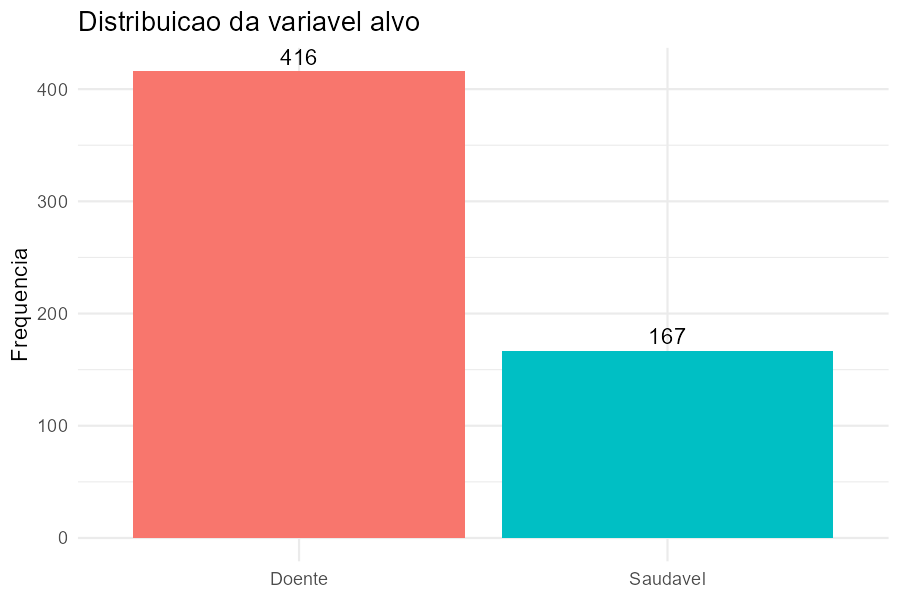
\includegraphics[width=0.7\textwidth]{figuras/cap4-metodologia/eda_distribuicao_alvo.png}
\caption{Distribuição da variável-alvo (doentes \textit{vs.} saudáveis).}
\label{fig:eda_distribuicao_alvo}
\end{figure}

Também se construiu uma tabela de contingência entre o sexo do paciente e a 
variável-alvo. A base é composta majoritariamente por pacientes do sexo masculino 
(cerca de 76\%). Esse desequilíbrio é relevante para o objetivo de interpretabilidade 
deste trabalho: se um grupo demográfico está sub-representado, o modelo pode ter 
desempenho desigual entre os grupos e aprender relações enviesadas \cite{Rajkomar2018Ensuring, investigatingbiashealth}. Por esse 
motivo, a avaliação dos modelos e a análise de interpretabilidade foram feitas também 
de forma estratificada por sexo.

\subsection{Estatísticas Descritivas e Assimetria}
\label{sec:estatisticas_descritivas_assimetria}

Para cada uma das nove variáveis numéricas foram calculadas a média, o 
desvio-padrão, o mínimo, a mediana, o máximo e o coeficiente de assimetria 
(\textit{skewness}), apresentados na Tabela~\ref{tab:descritivas}. A 
comparação entre média e mediana é especialmente informativa: como a mediana 
é pouco afetada por valores extremos, uma média muito superior à mediana 
indica que poucos valores elevados estão deslocando a média para cima 
\cite{gettintoknowyourdata}.

Para quantificar a assimetria de forma objetiva, utilizou-se o coeficiente 
de assimetria amostral, definido como o terceiro momento padronizado:

\begin{equation}
    b_1 = \frac{1}{n}\sum_{i=1}^{n}\left(\frac{x_i - \bar{x}}{s}\right)^3,
    \label{eq:assimetria}
\end{equation}

\noindent em que $n$ é o número de observações não ausentes, $\bar{x}$ é a 
média amostral e $s$ é o desvio-padrão amostral, calculado com denominador 
$n-1$. Como cada desvio é elevado ao cubo, o sinal é preservado e os valores 
mais distantes da média passam a dominar a soma. Em distribuições simétricas, 
as contribuições positivas e negativas se compensam e $b_1$ fica próximo de 
zero; valores positivos indicam cauda longa à direita. Existem variantes 
desse coeficiente que diferem apenas na correção para o tamanho da amostra, 
mas, para o $n$ deste estudo, as diferenças entre elas são desprezíveis \cite{Joanes1998Comparing}.

\begin{table}[htbp]
\centering
\caption{Estatísticas descritivas das variáveis numéricas do ILPD (base original, $n = 583$).}
\label{tab:descritivas}
\begin{tabular}{lrrrrrr}
\hline
\textbf{Variável} & \textbf{Média} & \textbf{DP} & \textbf{Mín.} & \textbf{Mediana} & \textbf{Máx.} & \textbf{$b_1$} \\
\hline
Age                         & 44,75  & 16,19  & 4    & 45   & 90    & $-0{,}03$ \\
Total\_Bilirubin            & 3,30   & 6,21   & 0,4  & 1,0  & 75,0  & 4,88 \\
Direct\_Bilirubin           & 1,49   & 2,81   & 0,1  & 0,3  & 19,7  & 3,20 \\
Alkaline\_Phosphotase       & 290,58 & 242,94 & 63   & 208  & 2110  & 3,75 \\
Alamine\_Aminotransferase   & 80,71  & 182,62 & 10   & 35   & 2000  & 6,52 \\
Aspartate\_Aminotransferase & 109,91 & 288,92 & 10   & 42   & 4929  & 10,49 \\
Total\_Proteins             & 6,48   & 1,09   & 2,7  & 6,6  & 9,6   & $-0{,}28$ \\
Albumin                     & 3,14   & 0,80   & 0,9  & 3,1  & 5,5   & $-0{,}04$ \\
AG\_Ratio\textsuperscript{a} & 0,95  & 0,32   & 0,3  & 0,93 & 2,8   & 0,99 \\
\hline
\multicolumn{7}{l}{\footnotesize DP: desvio-padrão; $b_1$: coeficiente de assimetria (Equação~\ref{eq:assimetria}).} \\
\multicolumn{7}{l}{\footnotesize \textsuperscript{a} Calculado sobre as 579 observações não ausentes.} \\
\end{tabular}
\end{table}

Adotou-se o critério $|b_1| > 2$ para identificar desvios substanciais da 
normalidade, valor a partir do qual \citeonline[p.~26]{curran1996robustness} 
observaram problemas significativos em procedimentos estatísticos, 
classificando distribuições com assimetria 2,0 como moderadamente 
não normais e com assimetria 3,0 como severamente não normais 
\cite[p.~20]{curran1996robustness}. Cinco variáveis ultrapassaram esse 
limiar: \textit{Total\_Bilirubin}, \textit{Direct\_Bilirubin}, 
\textit{Alkaline\_Phosphotase}, \textit{Alamine\_Aminotransferase} e 
\textit{Aspartate\_Aminotransferase}, com coeficientes entre 3,20 e 10,49, 
todos superiores inclusive ao nível de não normalidade severa. As demais 
variáveis não ultrapassaram 1,0 em valor absoluto. Dada essa separação 
nítida, a seleção das variáveis a serem transformadas não depende da 
escolha exata do limiar.

Esse comportamento é esperado do ponto de vista clínico. Em indivíduos 
saudáveis, bilirrubinas e enzimas hepáticas permanecem em faixas estreitas de 
referência, mas, em pacientes com lesão ou disfunção hepática, podem atingir 
valores várias vezes acima do limite superior da normalidade \cite{Giannini2005Liver, Kwo2016ACG}. Os 
valores extremos, portanto, não são erros de medição, e sim a própria 
manifestação laboratorial da doença que se deseja predizer. Removê-los 
significaria descartar justamente os casos mais informativos. Por isso, 
decidiu-se \textbf{não remover os \textit{outliers}} dessas variáveis \cite{Aggarwal2015}.

\subsection{Comparação entre Classes}

Para uma primeira avaliação do poder discriminativo de cada variável, compararam-se 
as médias dos grupos de pacientes doentes e saudáveis com o \textbf{teste $t$ de 
Welch}. Esse teste foi escolhido no lugar do teste $t$ de Student clássico porque não 
supõe que as variâncias dos dois grupos sejam iguais. Essa suposição seria pouco 
plausível aqui, dada a maior dispersão dos exames no grupo de doentes e a diferença 
de tamanho entre os grupos \cite{psychologists}. Considerou-se o nível de significância de 5\%.

Das nove variáveis analisadas, oito apresentaram diferença estatisticamente 
significativa entre as classes ($p < 0{,}05$), e apenas a variável 
\textit{Total\_Proteins} não apresentou diferença significativa 
($p = 0{,}393$), conforme detalhado na Tabela~\ref{tab:teste_welch}.

\begin{table}[htbp]
\centering
\caption{Resultado do teste $t$ de Welch entre as classes doente e saudável.}
\label{tab:teste_welch}
\begin{tabular}{lrrrl}
\hline
\textbf{Variável} & \textbf{Média Doente} & \textbf{Média Saudável} & \textbf{$p$-valor} & \textbf{Signif.} \\
\hline
Age                         & 46,15  & 41,24 & 0,0014   & sim \\
Total\_Bilirubin            & 4,16   & 1,14  & $<0{,}001$ & sim \\
Direct\_Bilirubin           & 1,92   & 0,40  & $<0{,}001$ & sim \\
Alkaline\_Phosphotase       & 319,01 & 219,75 & $<0{,}001$ & sim \\
Alamine\_Aminotransferase   & 99,61  & 33,65 & $<0{,}001$ & sim \\
Aspartate\_Aminotransferase & 137,70 & 40,69 & $<0{,}001$ & sim \\
Total\_Proteins             & 6,46   & 6,54  & 0,3932   & não \\
Albumin                     & 3,06   & 3,34  & $<0{,}001$ & sim \\
AG\_Ratio                   & 0,91   & 1,03  & $<0{,}001$ & sim \\
\hline
\end{tabular}
\end{table}

Essa análise é univariada: avalia cada variável isoladamente e não considera 
interações nem efeitos combinados, que são justamente o que os modelos de aprendizado 
de máquina conseguem capturar. Além disso, por causa da forte assimetria de algumas 
variáveis, os resultados do teste devem ser lidos com cautela. Ainda assim, o teste 
de Welch tende a ser robusto a desvios de normalidade em amostras deste tamanho, 
pelo Teorema Central do Limite \cite{theimportanceofnormality}. Os resultados servem como referência para 
comparar, no Capítulo de Resultados, com as importâncias de atributos obtidas por 
meio dos valores SHAP.

Também foram gerados \textit{boxplots} de cada variável numérica, separados por 
classe (Figura~\ref{fig:eda_boxplots}). Eles permitem inspecionar visualmente a sobreposição entre as
distribuições dos dois grupos e a presença de valores extremos. Uma grande 
sobreposição entre as classes indica que nenhum exame, sozinho, separa bem doentes de 
saudáveis, o que motiva o uso de modelos multivariados.

\begin{figure}[htbp]
\centering
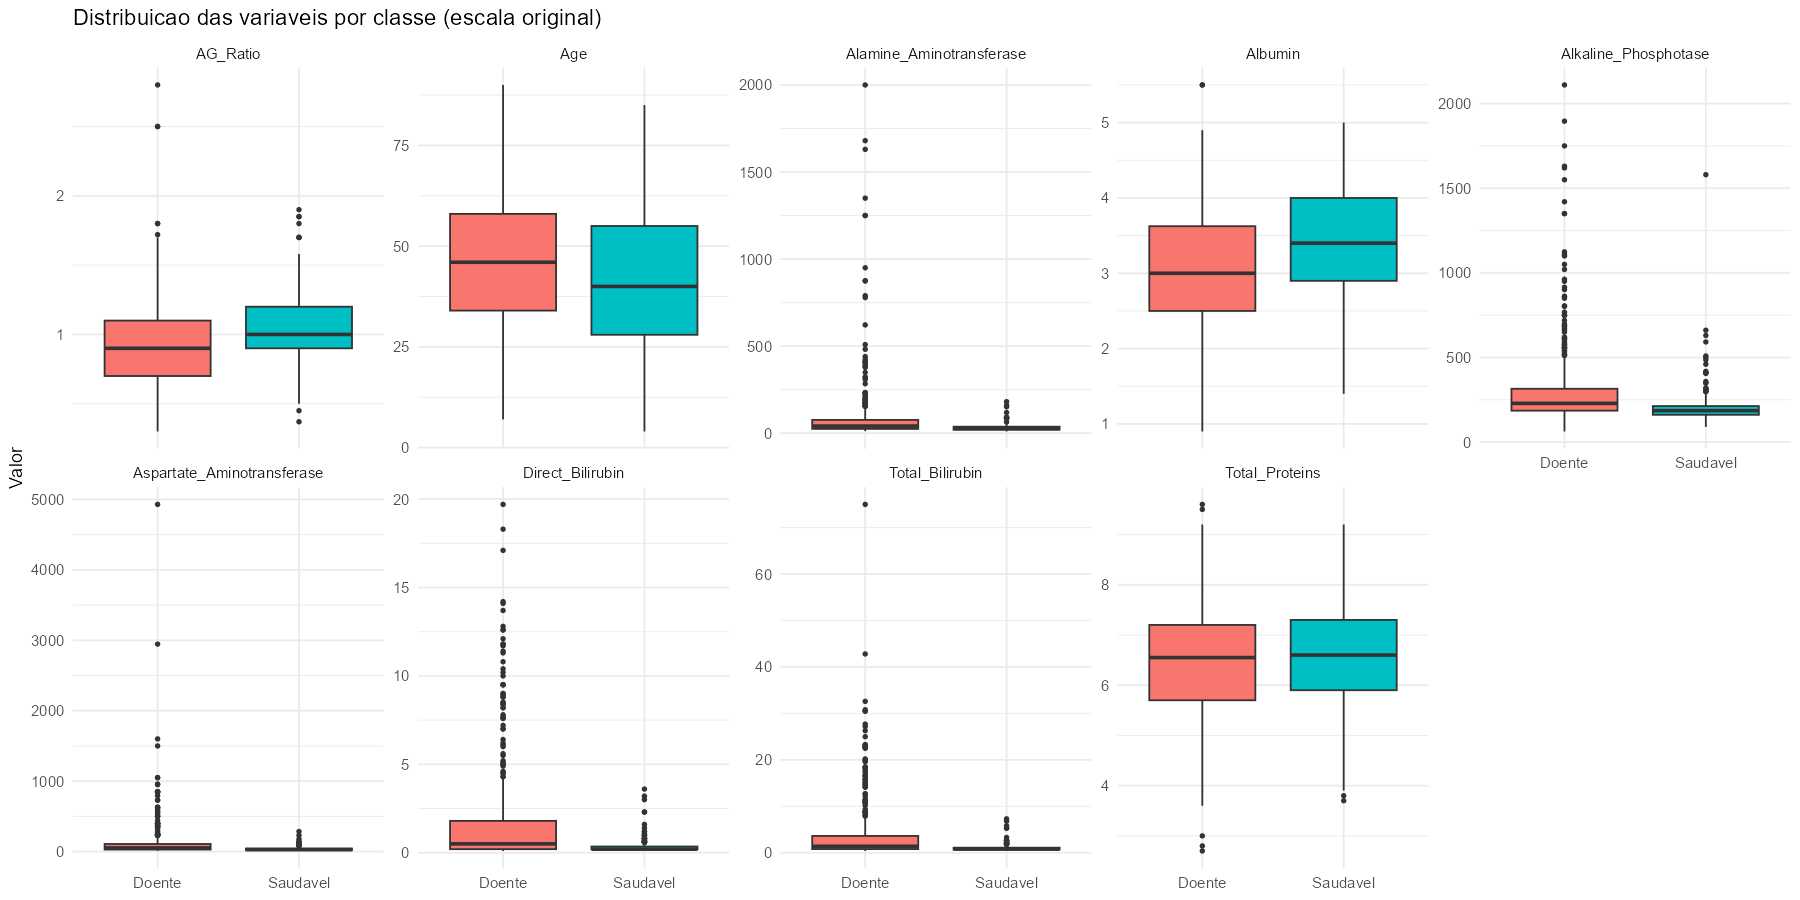
\includegraphics[width=\textwidth]{figuras/cap4-metodologia/eda_boxplots_por_classe.png}
\caption{Boxplots das variáveis numéricas, separados por classe (doente \textit{vs.} saudável).}
\label{fig:eda_boxplots}
\end{figure}

\subsection{Análise de Correlação}

Por fim, calculou-se a matriz de correlação de Pearson entre as variáveis numéricas 
(Figura~\ref{fig:eda_correlacao}). As observações com valores ausentes foram excluídas apenas para esse
cálculo. O objetivo foi identificar \textbf{multicolinearidade}, ou seja, pares de 
variáveis que carregam praticamente a mesma informação. Adotou-se $|r| > 0{,}7$ como 
limiar de correlação forte \cite{Dormann2012Collinearity, Mukaka2012Statistics}.

\begin{figure}[htbp]
\centering
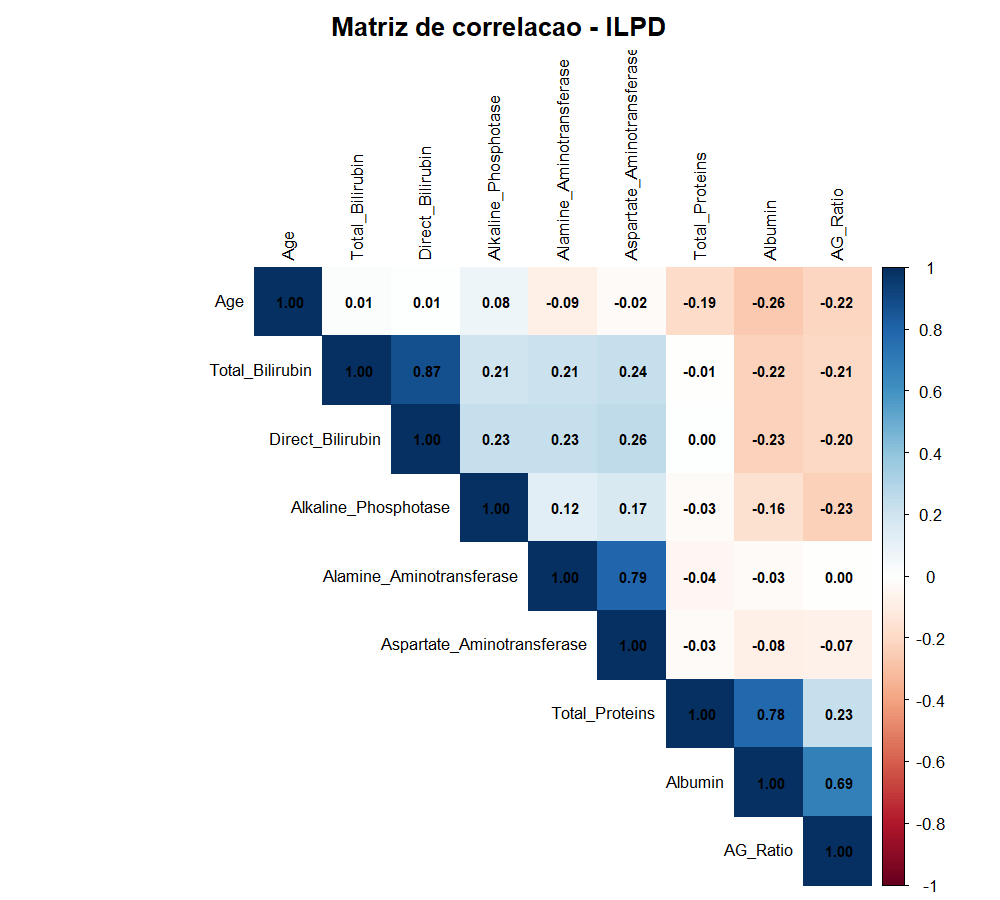
\includegraphics[width=0.8\textwidth]{figuras/cap4-metodologia/eda_correlacao.png}
\caption{Matriz de correlação de Pearson entre as variáveis numéricas.}
\label{fig:eda_correlacao}
\end{figure}

Encontrou-se correlação forte nos pares \textit{Total\_Bilirubin} × 
\textit{Direct\_Bilirubin} ($r = 0{,}874$), \textit{Alamine\_Aminotransferase} × 
\textit{Aspartate\_Aminotransferase} ($r = 0{,}792$) e \textit{Total\_Proteins} × 
\textit{Albumin} ($r = 0{,}783$). Essas correlações têm explicação fisiológica: 
a bilirrubina direta é uma das frações que compõem a bilirrubina total 
\cite{Fevery2008Bilirubin, Kwo2016ACG}, e a razão albumina/globulina é derivada 
da albumina e das proteínas totais, uma vez que a globulina é obtida pela 
diferença entre as duas \cite{Busher1990Albumin, Newsome2018Guidelines}.

Mesmo com essa redundância, optou-se por \textbf{manter todas as variáveis}. A decisão 
tem três motivos:
\begin{enumerate}
    \item Os modelos baseados em árvores (\textit{Random Forest}, XGBoost e LightGBM) 
    são, em geral, robustos à multicolinearidade quanto ao desempenho preditivo 
    \cite{Breiman2001RandomForests, Chen2016XGBoost, Ke2017LightGBM}. Em estudo de 
    simulação com diferentes níveis de colinearidade, \citeonline{Dormann2012Collinearity} 
    observaram que \textit{Random Forest} e árvores com \textit{boosting} mantiveram 
    desempenho estável em dados de teste, degradando apenas sob correlações extremas 
    ou quando a estrutura de correlação muda entre treino e teste, situação que não 
    se aplica a este trabalho, pois treino e teste provêm da mesma base;
    \item Excluir variáveis clinicamente relevantes contraria o objetivo de 
    interpretabilidade deste trabalho, que é entender como os modelos usam os exames 
    laboratoriais disponíveis;
    \item A multicolinearidade afeta principalmente a \textit{interpretação} dos 
    modelos, não sua capacidade preditiva \cite{Strobl2008Conditional, Dormann2012Collinearity}. 
    No caso do método SHAP, a presença de variáveis correlacionadas pode levar à 
    divisão da importância entre elas: como o modelo pode usar qualquer uma das 
    variáveis redundantes para capturar a mesma informação, o crédito atribuído a 
    cada uma individualmente tende a se diluir \cite{Aas2021Explaining, Chen2023Algorithms, Verdinelli2024Feature}. 
    Esse efeito é particularmente relevante na variante do TreeSHAP utilizada 
    neste trabalho para o XGBoost e o LightGBM, que estima as contribuições a 
    partir da estrutura das próprias árvores e das frequências de passagem pelos 
    nós, aproximando a distribuição condicional das variáveis 
    \cite{Lundberg2020Trees, Chen2023Algorithms}. Já para o \textit{Random Forest}, 
    cujos valores SHAP foram estimados por amostragem de Monte Carlo com permutação 
    marginal, as variáveis são tratadas como independentes, o que evita a divisão 
    de crédito mas pode avaliar o modelo em combinações de valores pouco plausíveis 
    quando há dependência \cite{Chen2020TrueToModel}. Essa diferença entre 
    estimadores é considerada explicitamente na discussão dos resultados.
\end{enumerate}

Como limitação, o coeficiente de Pearson mede apenas associações lineares e é 
sensível a valores extremos: um único ponto atípico pode alterar substancialmente a 
magnitude e até o sinal do coeficiente \cite{Schober2018Correlation}. 
Como as correlações foram calculadas na escala original, a presença de variáveis 
muito assimétricas pode ter influenciado a magnitude dos coeficientes, uma vez que 
distribuições com caudas pesadas tendem a inflar o valor de $r$ 
\cite{Bishara2015Reducing}.

\section{Pré-processamento}

\subsection{Remoção de Duplicatas}

Os 13 registros duplicados identificados na análise exploratória foram removidos, 
e a base passou de 583 para 570 registros.

\subsection{Transformação Logarítmica}

Às cinco variáveis assimétricas identificadas na análise exploratória aplicou-se a 
transformação $x' = \ln(1 + x)$ (Seção~\ref{sec:estatisticas_descritivas_assimetria}) \cite{logtransformation}. O logaritmo comprime a cauda da
distribuição sem alterar a ordem entre as observações: na 
\textit{Aspartate\_Aminotransferase}, por exemplo, o máximo, que era mais de 
cem vezes maior que a mediana na escala original, passa a ser cerca de duas 
vezes maior na escala transformada. Após a transformação, calculada sobre a 
base já sem os registros duplicados ($n = 570$), os coeficientes de 
assimetria passaram a variar entre 1,24 e 1,72, todos abaixo do limiar 
adotado (Tabela~\ref{tab:assimetria_log}). A soma de uma unidade antes do 
logaritmo garante que a transformação seja bem definida para valores 
próximos de zero, como os da \textit{Direct\_Bilirubin} (mínimo de 0,1 mg/dL).

Observe-se que os valores da coluna ``Antes'' da Tabela~\ref{tab:assimetria_log} 
diferem ligeiramente dos apresentados na Tabela~\ref{tab:descritivas}. A diferença 
não é um erro: a Tabela~\ref{tab:descritivas} descreve a base original completa 
($n = 583$), enquanto a Tabela~\ref{tab:assimetria_log} foi calculada após a 
remoção dos 13 registros duplicados ($n = 570$), que é a base efetivamente usada 
no pré-processamento. Como o coeficiente de assimetria é sensível à composição 
exata da amostra, a exclusão de poucas observações já produz pequenas variações 
nas casas decimais, sem alterar nenhuma das conclusões.

Cabe ainda um esclarecimento sobre o momento em que essa transformação é aplicada. 
Diferentemente da imputação pela mediana e da padronização, que dependem de 
parâmetros estimados a partir dos dados (mediana, média e desvio-padrão do 
treino), a transformação $\ln(1+x)$ é \textbf{determinística e livre de 
parâmetros}: o valor transformado de cada observação depende exclusivamente 
dela mesma, e não de nenhuma estatística do conjunto. Por isso, aplicá-la antes 
da divisão treino/teste, como foi feito neste trabalho, não introduz vazamento 
de dados, pois nenhuma informação do conjunto de teste é usada para definir a 
transformação \cite{KaufmanScharRosset2012}. O mesmo não valeria, por exemplo, 
para uma transformação de Box-Cox, cujo expoente $\lambda$ é estimado a partir 
dos dados e, portanto, deveria ser ajustado apenas no treino.

\begin{table}[htbp]
\centering
\caption{Coeficiente de assimetria ($b_1$) antes e depois da transformação $\ln(1+x)$ ($n = 570$).}
\label{tab:assimetria_log}
\begin{tabular}{lrr}
\hline
\textbf{Variável} & \textbf{Antes} & \textbf{Depois} \\
\hline
Total\_Bilirubin            & 4,84  & 1,72 \\
Direct\_Bilirubin           & 3,17  & 1,68 \\
Alkaline\_Phosphotase       & 3,71  & 1,32 \\
Alamine\_Aminotransferase   & 6,66  & 1,46 \\
Aspartate\_Aminotransferase & 10,50 & 1,24 \\
\hline
\end{tabular}
\end{table}

A transformação é especialmente relevante para a Regressão Logística, que 
assume relação linear entre os preditores e o logaritmo da razão de chances 
e é sensível a observações extremas \cite{Hosmer2005Applied}. Na escala logarítmica, o efeito 
de cada exame passa a depender de variações proporcionais, como dobrar o 
valor de uma enzima, o que é mais coerente com a interpretação clínica desses 
marcadores. Já os modelos baseados em árvores de decisão são, em princípio, 
invariantes a transformações monotônicas, pois suas divisões dependem apenas 
da ordem dos valores \cite{elementsofstatiscal}. Ainda assim, a transformação foi aplicada a 
todos os modelos, para que fossem comparados sobre a mesma representação dos 
dados, o que também facilita a leitura dos gráficos de dependência SHAP, nos 
quais os pacientes passam a se distribuir de forma mais uniforme ao longo do 
eixo horizontal.

\subsection{Divisão Treino/Teste}
\label{sec:divisao_treino_teste}

Após as transformações determinísticas, os dados foram divididos em conjuntos
de treino e teste na proporção de 80\% e 20\%, respectivamente, por meio da
função \texttt{createDataPartition} do pacote \texttt{caret}. A divisão foi
estratificada pela variável-alvo, preservando a proporção das classes em ambos
os conjuntos. Uma semente aleatória fixa, definida uma única vez no início do
\textit{pipeline}, garante a reprodutibilidade dessa partição. Essa divisão
ocorre antes da imputação e da padronização, de modo que os parâmetros dessas
duas etapas sejam estimados exclusivamente no conjunto de treino, evitando o
vazamento de informação do conjunto de teste \cite{KaufmanScharRosset2012}.

\subsection{Imputação de Valores Ausentes}

A mediana foi calculada exclusivamente no conjunto de treino e depois aplicada a 
ambos os conjuntos (Seção~\ref{sec:divisao_treino_teste}).

\subsection{Padronização}
\label{sec:padronizacao}

Após a imputação, os preditores foram padronizados pela transformação
\textit{z-score}, com centralização (\textit{center}) e escalonamento
(\textit{scale}). As médias e os desvios-padrão foram estimados exclusivamente
no conjunto de treino e, em seguida, aplicados tanto ao treino quanto ao teste,
mantendo a separação entre os dados usados para ajustar os parâmetros e os
usados para avaliação. Essa etapa é particularmente relevante para a Regressão
Logística, um modelo linear sensível às escalas dos preditores; para os modelos
baseados em árvores, que realizam divisões pela ordem dos valores, a
padronização tende a ser menos relevante.

\subsection{Balanceamento de Classes (SMOTE)}
\label{sec:balanceamento}

Para lidar com o desbalanceamento das classes, utilizou-se o SMOTE
(\textit{Synthetic Minority Over-sampling Technique})\cite{smote}, que gera amostras
sintéticas da classe minoritária a partir de observações existentes. O
balanceamento é aplicado somente aos dados de treino; o conjunto de teste
mantém sua distribuição original e nunca é balanceado. Durante o treinamento
com validação cruzada, o SMOTE é aplicado independentemente dentro de cada
partição de treino de cada \textit{fold}, após a separação dos \textit{folds}.
Assim, as amostras sintéticas não contaminam as partições de validação — o que
poderia ocorrer se o balanceamento fosse feito antes da divisão — nem inflacionam
artificialmente as métricas de desempenho.

\section{Modelos Preditivos}

Foram comparados quatro classificadores com diferentes graus de flexibilidade:
um modelo linear, empregado como referência interpretável, e três métodos
baseados em árvores, capazes de representar relações não lineares e interações
entre os preditores. Essa comparação permite examinar se a maior flexibilidade
dos modelos de conjunto oferece vantagens preditivas em relação a uma
abordagem linear, sem pressupor de antemão qual método terá o melhor
desempenho. A classe positiva considerada no treinamento é ``doente''.

\subsection{Regressão Logística}

A Regressão Logística modela a probabilidade de pertencimento à classe positiva
por meio da função logística aplicada a uma combinação linear dos preditores.
Embora seja um classificador linear na escala dos logitos, a transformação
logística produz probabilidades entre zero e um. Seus coeficientes descrevem
a variação nos logitos associada aos preditores, mantidos os demais constantes;
a exponenciação de cada coeficiente fornece a correspondente razão de chances
(\textit{odds ratio}) \cite{Hosmer2005Applied, elementsofstatiscal}.

Neste estudo, ajustou-se o modelo binomial sem busca de hiperparâmetros. Ele foi
incluído como \textit{baseline} por combinar uma formulação estatística
conhecida com interpretação direta dos coeficientes, oferecendo um ponto de
comparação para os métodos de árvores. Como os preditores numéricos foram
padronizados, os coeficientes correspondem a variações de uma unidade na escala
padronizada; suas exponenciais são apresentadas como razões de chances.

\subsection{Random Forest}

O Random Forest constrói um conjunto de árvores de decisão a partir de
reamostragens dos dados e de subconjuntos aleatórios de preditores considerados
nas divisões. Para classificação, as árvores contribuem para a previsão
agregada do conjunto. A aleatorização e a agregação visam reduzir a variância
em relação a uma árvore individual, preservando a capacidade de representar
relações não lineares \cite{Breiman2001RandomForests}.

Esse método foi incluído por oferecer uma estratégia de \textit{bagging}
robusta e não linear, distinta do ajuste aditivo por boosting dos outros
métodos de árvores. No treinamento, foram utilizadas 500 árvores; os demais
parâmetros considerados pelo classificador foram selecionados no procedimento
de busca descrito na seção seguinte.

\subsection{XGBoost}

O XGBoost é um método de \textit{gradient boosting} que constrói árvores
sequencialmente: cada nova etapa busca reduzir a função de perda, levando em
conta os erros do conjunto de árvores já ajustado. A implementação acrescenta
recursos de regularização e eficiência computacional ao processo de
aprendizado de árvores \cite{Chen2016XGBoost}.

Sua inclusão permite avaliar uma abordagem de boosting amplamente utilizada,
com mecanismos de regularização e uma implementação otimizada, em contraste
com a agregação por reamostragem do Random Forest. Os parâmetros da variante
de árvores do XGBoost foram selecionados por busca aleatória, conforme o
protocolo de treinamento.

\subsection{LightGBM}

O LightGBM é outro método de \textit{gradient boosting} baseado em árvores,
projetado para treinar de forma eficiente em conjuntos de dados de maior
dimensão. Sua estratégia de crescimento das árvores e suas técnicas de
amostragem e representação de atributos buscam reduzir o custo computacional
sem abandonar o ajuste sequencial característico do boosting
\cite{Ke2017LightGBM}.

O método foi incluído para comparar uma implementação de boosting com
estratégia de eficiência distinta à do XGBoost. Como o ambiente de treinamento
utilizado não oferece suporte nativo ao LightGBM, a integração foi feita por
meio de um adaptador compatível com a interface de treinamento empregada no
pipeline; seus hiperparâmetros foram submetidos à mesma busca aleatória dos
demais modelos ajustáveis.

\section{Treinamento e Validação Cruzada}

O treinamento e a seleção de modelos foram conduzidos apenas com o conjunto de
treino, preservando o conjunto de teste separado para a avaliação final. Para
estimar o desempenho durante o desenvolvimento, utilizou-se validação cruzada
repetida, com cinco partições (\textit{folds}) e três repetições. Em cada
rodada, quatro partições são usadas para ajuste e a partição restante para
validação; as repetições submetem os modelos a partições distintas e reduzem
a dependência dos resultados em relação a uma única divisão aleatória dos
dados.

Nos modelos que possuem parâmetros de ajuste, foram avaliadas 30 combinações
amostradas por busca aleatória. Em comparação com uma grade exaustiva, a busca
aleatória permite explorar valores distintos em cada dimensão do espaço de
hiperparâmetros, sem exigir a avaliação de todas as combinações cartesianas;
essa abordagem é particularmente útil quando apenas parte dos parâmetros
influencia fortemente o desempenho \cite{}% TODO: buscar Bergstra e Bengio (2012), “Random Search for Hyper-Parameter Optimization”. Prompt para Consensus: “Qual é o artigo de Bergstra e Bengio, publicado em 2012, que compara busca aleatória e busca em grade para otimização de hiperparâmetros, e quais são seus principais argumentos de eficiência?”
A Regressão Logística, ajustada sem hiperparâmetros a otimizar, não requer essa
busca.

A seleção dos modelos e das combinações de hiperparâmetros foi baseada na área
sob a curva ROC (AUC-ROC), calculada a partir das probabilidades estimadas para
a classe positiva. A AUC resume a capacidade de ordenação dos casos positivos
acima dos negativos ao longo dos limiares, sem depender de um único ponto de
corte. Por isso, complementa a acurácia, que pode ser enganosa quando as
classes têm frequências diferentes: como discutido na Análise Exploratória,
um classificador pode obter acurácia aparentemente alta favorecendo a classe
mais frequente sem discriminar adequadamente os casos da classe minoritária
\cite{FAWCETT2006861, imbalancedata}.

O desbalanceamento foi tratado dentro do procedimento de reamostragem: em cada
\textit{fold}, o SMOTE é aplicado somente à partição usada para ajustar o
modelo, depois da separação da partição de validação. Dessa forma, as
observações sintéticas não são compartilhadas com a validação, evitando
vazamento de informação e mantendo a estimativa de desempenho baseada em dados
não balanceados artificialmente.

Ao final da validação cruzada, os resultados dos quatro modelos foram
comparados pela distribuição das AUCs nos \textit{folds}, apresentada em
gráfico de caixas, e por testes t pareados com correção de Bonferroni para as
comparações entre pares. A comparação pareada considera que os modelos foram
avaliados nas mesmas partições; a correção de Bonferroni controla o aumento do
erro tipo I decorrente das comparações múltiplas. A literatura sobre
comparação estatística de classificadores discute as escolhas e limitações
desses procedimentos \cite{}% TODO: buscar Janez Demšar (2006), “Statistical Comparisons of Classifiers over Multiple Data Sets”. Prompt para Consensus: “Quais procedimentos estatísticos Demšar recomenda em 2006 para comparar classificadores e quais são as limitações de testes pareados sobre resultados de validação cruzada?”

\section{Avaliação de Desempenho}

Após a seleção e o ajuste dos modelos, o desempenho foi medido no conjunto de
teste, que não participou do treinamento, da seleção de hiperparâmetros nem da
geração de amostras SMOTE. Esse conjunto manteve a distribuição observada das
classes, de modo que as métricas finais reflitam a prevalência original dos
dados e não uma distribuição artificialmente balanceada. Para cada modelo,
foram obtidas as previsões de classe e as probabilidades estimadas para
``doente''.

A matriz de confusão resume verdadeiros positivos, verdadeiros negativos,
falsos positivos e falsos negativos para um limiar de decisão. No limiar padrão
de 0,5, a partir dela foram calculadas a acurácia, a acurácia balanceada, a
sensibilidade, a especificidade, a precisão, a medida F1 e a estatística Kappa;
a AUC-ROC foi calculada a partir das probabilidades. A sensibilidade corresponde à
proporção de doentes identificados, enquanto a especificidade corresponde à
proporção de não doentes identificados. A precisão expressa a proporção de
previsões positivas que são de fato positivas, e a medida F1 resume o
equilíbrio entre precisão e sensibilidade. A acurácia balanceada dá peso
igual à sensibilidade e à especificidade, e o Kappa expressa a concordância
entre classe prevista e observada descontada a concordância esperada ao acaso.
Para a AUC de cada modelo, foram calculados intervalos de confiança de 95\%
pelo método de DeLong.

Considerar a acurácia isoladamente seria inadequado diante do desbalanceamento
identificado na AED: ela pode ser dominada pelo desempenho na classe mais
frequente e ocultar erros na classe minoritária. Por essa razão, a avaliação
considera conjuntamente métricas por classe, acurácia balanceada e AUC, em
consonância com a discussão sobre curvas ROC e classificação em bases
desbalanceadas \cite{FAWCETT2006861, imbalancedata}. Também foram construídas
curvas Precision--Recall. Como elas relacionam precisão e sensibilidade da
classe positiva, complementam a curva ROC ao tornar explícito o compromisso
entre encontrar casos doentes e limitar os falsos positivos em um cenário no
qual a prevalência da classe positiva não é majoritária.

Além do limiar padrão de 0,5, foram examinados dois critérios de decisão. O
primeiro é o limiar que maximiza o índice de Youden, definido pela soma da
sensibilidade e da especificidade menos um. O segundo é um limiar clínico
escolhido para garantir sensibilidade de pelo menos 90\%, selecionando, entre
os limiares que atendem a essa meta, aquele que preserva a maior especificidade
possível. Essa análise prioriza a redução de falsos negativos — pacientes
doentes classificados como não doentes —, erro considerado especialmente
crítico em um cenário de triagem clínica, no qual um resultado negativo
equivocado pode atrasar a investigação diagnóstica \cite{}% TODO: buscar literatura de diagnóstico médico sobre custo assimétrico de falsos negativos e priorização de sensibilidade em triagem. Prompt para Consensus: “Que estudos ou diretrizes de diagnóstico clínico discutem o custo de falsos negativos e justificam priorizar alta sensibilidade em testes de triagem médica?”

As AUCs dos quatro modelos no conjunto de teste também foram comparadas em
pares pelo teste de DeLong para curvas ROC. O método permite avaliar a
diferença entre áreas sem tratar as estimativas das curvas como independentes
quando são obtidas nos mesmos pacientes \cite{}% TODO: buscar Elizabeth R. DeLong, David M. DeLong e Daniel L. Clarke-Pearson (1988), “Comparing the Areas under Two or More Correlated Receiver Operating Characteristic Curves: A Nonparametric Approach”. Prompt para Consensus: “Qual método não paramétrico DeLong, DeLong e Clarke-Pearson propuseram em 1988 para comparar as áreas sob duas ou mais curvas ROC correlacionadas?”

Por fim, as métricas foram calculadas separadamente para pacientes do sexo
feminino e masculino, como continuação da preocupação com a predominância
masculina observada na AED. Para cada grupo foram estimadas AUC e seu intervalo
de confiança de 95\%, sensibilidade e especificidade. A diferença de AUC entre
os grupos foi avaliada pelo teste de DeLong para amostras independentes, e
também foram examinadas as diferenças de sensibilidade e especificidade. Essa
estratificação permite identificar possíveis disparidades de desempenho e
risco desigual de falsos negativos, sem, por si só, estabelecer sua causa;
essa auditoria é relevante diante das preocupações com viés algorítmico em
saúde \cite{Rajkomar2018Ensuring, investigatingbiashealth}. As diferenças
devem ser interpretadas com cautela, considerando a quantidade de observações
disponíveis em cada grupo.

\section{Interpretabilidade com SHAP}

Os valores SHAP (\textit{SHapley Additive exPlanations}) adaptam os valores de
Shapley da teoria dos jogos cooperativos para atribuir a cada preditor uma
contribuição à previsão de um modelo. Para uma observação, cada contribuição
representa a parcela associada à variável na diferença entre uma previsão de
referência e a previsão obtida para aquela observação, segundo a definição do
valor de Shapley. Essa formulação fornece explicações locais aditivas, que
podem também ser agregadas para descrever padrões globais \cite{}% TODO: buscar Scott M. Lundberg e Su-In Lee (2017), “A Unified Approach to Interpreting Model Predictions”, artigo original que introduziu SHAP. Prompt para Consensus: “Qual artigo de Lundberg e Lee, publicado em 2017, introduziu SHAP como uma abordagem unificada para interpretar previsões de modelos de machine learning?”

O cálculo depende do tipo de modelo. Para XGBoost e LightGBM, foram usados
valores TreeSHAP exatos, obtidos pelas contribuições nativas das árvores. No
fluxo adotado, essas contribuições estão na escala de logitos (\textit{log-odds});
valores positivos deslocam a previsão em direção à classe ``doente'' e valores
negativos em direção à classe ``saudável''. TreeSHAP permite calcular as
atribuições para modelos de árvores explorando sua estrutura
\cite{Lundberg2020Trees}.

Para o Random Forest, utilizou-se o pacote \textit{fastshap} para obter uma
estimativa amostral de SHAP por Monte Carlo, com 100 simulações por explicação
e na escala de probabilidade. Essa
escolha decorre de o fluxo utilizado não dispor de TreeSHAP exato para o
Random Forest. A estimativa amostral aproxima as contribuições a partir de
coalizões de variáveis; diferentemente do cálculo TreeSHAP empregado para os
modelos de boosting, o procedimento adotado trata as variáveis como
independentes ao construir as amostras de referência. As diferenças de
algoritmo e de escala devem ser consideradas ao interpretar e comparar os
valores obtidos \cite{}% TODO: buscar o trabalho original sobre Kernel SHAP e amostragem de valores de Shapley, associado a Scott M. Lundberg e Su-In Lee (2017), “A Unified Approach to Interpreting Model Predictions”, e verificar a formulação de Shapley Sampling Values. Prompt para Consensus: “Qual publicação original descreve Kernel SHAP e a aproximação amostral dos valores de Shapley para explicar previsões de modelos, e como o método amostra coalizões de variáveis?”

Os coeficientes e respectivas razões de chances da Regressão Logística
fornecem uma representação direta dos efeitos estimados, de modo que esse
modelo não integra a seleção padrão de modelos a explicar. A regra também
inclui o melhor modelo no teste segundo a AUC; caso a Regressão Logística
ocupe essa posição, ela é incluída nessa seleção. Assim, são explicados o
XGBoost, o Random Forest e o melhor modelo no teste, removendo-se duplicatas.

Para cada modelo explicado, a importância global de uma variável é calculada
pela média do valor absoluto de SHAP entre os pacientes; ela resume a
magnitude média da contribuição, mas não informa sua direção. O gráfico
\textit{beeswarm} mostra a distribuição das contribuições individuais e
relaciona sua posição com os valores das variáveis, permitindo observar
heterogeneidade entre pacientes. A direção do efeito também é examinada pela
correlação entre o valor de cada variável e seu valor SHAP; essa associação é
descritiva e não deve ser interpretada como efeito causal. Para as quatro
variáveis de maior importância, gráficos de dependência mostram como as
contribuições variam ao longo dos valores observados. Por fim, gráficos
\textit{waterfall} decompõem previsões individuais em relação ao valor de
referência, mostrando como as contribuições de cada variável conduzem à
previsão do paciente.

As explicações locais são produzidas para três casos definidos a partir do
conjunto de teste: o verdadeiro positivo com maior probabilidade estimada de
doença, o verdadeiro negativo com menor probabilidade estimada de doença e o
falso negativo de pior erro, isto é, o paciente doente com menor probabilidade
estimada de pertencer à classe positiva. A seleção torna possível examinar
tanto previsões corretas de maior confiança quanto um caso particularmente
crítico de doença não identificada.

Como aprofundamento da avaliação de desempenho por sexo, a importância SHAP
também é calculada separadamente para os grupos feminino e masculino. A
concordância entre os rankings de importância de cada grupo é resumida pela
correlação de Spearman; adicionalmente, examina-se a contribuição SHAP média
com sinal da variável \textit{Gender} em cada grupo. Essas análises descrevem
se o modelo distribui e direciona suas contribuições de modo semelhante
entre os grupos, sem substituir a avaliação de disparidades de desempenho nem
permitir, isoladamente, inferências causais.

Por último, os rankings de importância são comparados entre os quatro
classificadores. Para XGBoost e Random Forest são consideradas as importâncias
SHAP; para Random Forest e LightGBM também se obtêm importâncias nativas dos
modelos, e para a Regressão Logística usa-se o valor absoluto dos coeficientes
padronizados. A concordância entre esses rankings é examinada por correlação
de Spearman. Como as medidas de importância têm definições e escalas
diferentes, a comparação enfatiza a ordenação relativa das variáveis, e não a
equivalência numérica das contribuições.
                 % metodo proposto e           resultados 
\chapter{Resultados} \label{cap:resultados}

Este capítulo apresenta os resultados de cada etapa do \textit{pipeline} descrito no Capítulo~\ref{metodologia}, na ordem em que foram executadas. Todos os números foram extraídos dos arquivos de resultados da execução com semente 42 e podem ser reproduzidos com o código disponibilizado.

% =============================================================================
\section{Análise Exploratória dos Dados}
\label{sec:res_aed}
% =============================================================================

Apenas \textit{AG\_Ratio} teve valores ausentes (4 registros, 0,69\% da base), e foram encontrados 13 registros exatamente duplicados. A base tem 416 doentes (71,4\%) e 167 saudáveis (Figura~\ref{fig:eda_distribuicao_alvo}), e 441 homens (75,6\%) e 142 mulheres. A proporção de doentes é maior entre os homens (73,5\%) do que entre as mulheres (64,8\%), o que impede comparar diretamente entre os sexos métricas que dependem da prevalência, como a precisão.

As maiores diferenças entre as classes (Tabela~\ref{tab:medias_classe}) estão nas bilirrubinas (média da direta cerca de 4,9 vezes maior nos doentes, e da total, 3,6 vezes) e nas aminotransferases (cerca de três vezes); \textit{Total\_Proteins} quase não difere (6,46 contra 6,54). Nos \textit{boxplots} (Figura~\ref{fig:eda_boxplots}), porém, as caixas de doentes e saudáveis se sobrepõem em todas as variáveis, de modo que nenhum exame sozinho separa bem as classes, o que motiva o uso de modelos multivariados.

Houve correlação forte em três pares (Figura~\ref{fig:eda_correlacao}): bilirrubina total e direta ($r = 0{,}874$), ALT e AST ($r = 0{,}792$) e proteínas totais e albumina ($r = 0{,}783$), todas com explicação fisiológica (Seção~\ref{sec:fund_figado}). Além disso, \textit{Total\_Proteins}, \textit{Albumin} e \textit{AG\_Ratio} são redundantes: como a globulina é a diferença entre proteínas totais e albumina, quaisquer duas delas determinam a terceira. Essa redundância reaparece na interpretação dos modelos (Seções~\ref{sec:res_coef_lr} e~\ref{sec:res_shap_global}).

% =============================================================================
\section{Pré-processamento}
\label{sec:res_preproc}
% =============================================================================

A remoção das duplicatas deixou 570 pacientes (406 doentes e 164 saudáveis). A transformação logarítmica reduziu a assimetria das cinco variáveis de 3,17--10,50 para 1,24--1,72 (Tabela~\ref{tab:assimetria_log}). A divisão resultou em 457 pacientes no treino e 113 no teste (71,1\% e 71,7\% de doentes; 32 mulheres e 81 homens no teste). Os quatro valores ausentes caíram no treino e foram imputados com a mediana (1,00).

\subsection{Reamostragem com SMOTE}
\label{sec:res_smote}

No treino completo, o SMOTE gerou 132 amostras sintéticas de pacientes saudáveis, e a razão entre as classes passou de cerca de 2,5:1 (325 doentes e 132 saudáveis) para 1,2:1 (325 e 264) (Figura~\ref{fig:res_smote}). As médias das amostras sintéticas ficaram a menos de 0,05 desvio-padrão das dos saudáveis originais, e apenas uma delas precisou ter o valor de \textit{Gender} corrigido.

\begin{figure}[htbp]
\centering
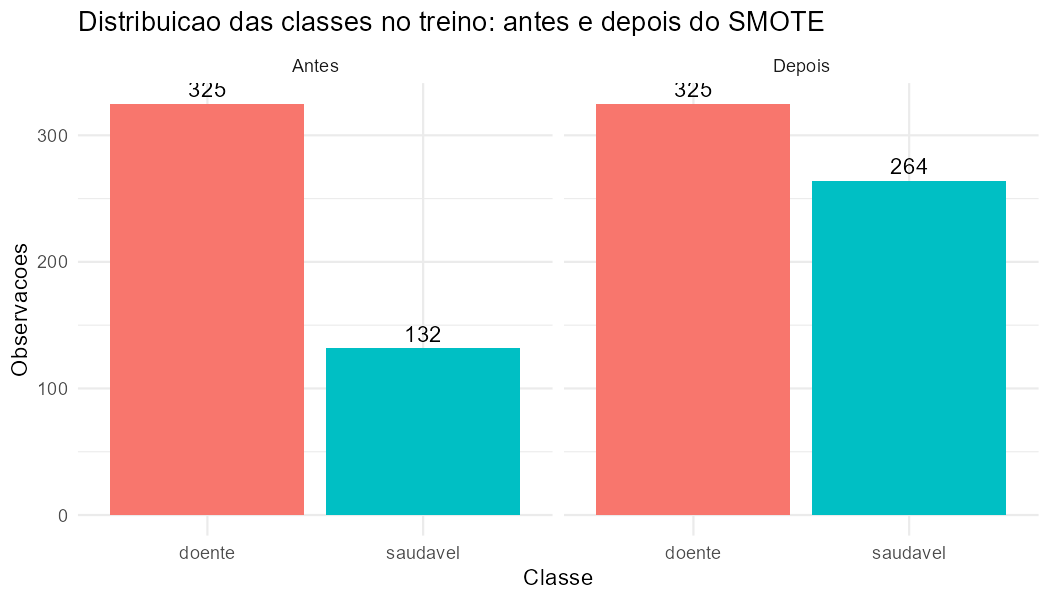
\includegraphics[width=0.6\textwidth]{figuras/cap5-resultados/smote_antes_depois.png}
\caption{Distribuição das classes no conjunto de treino antes e depois do SMOTE.}
\label{fig:res_smote}
\end{figure}

% =============================================================================
\section{Treinamento e Validação Cruzada}
\label{sec:res_cv}
% =============================================================================

\subsection{Hiperparâmetros Selecionados}

Os hiperparâmetros selecionados (Tabela~\ref{tab:res_hiper}) correspondem a modelos simples. No \textit{Random Forest}, venceu \texttt{mtry} = 1, isto é, cada divisão considera uma única variável sorteada. O XGBoost usa só 24 árvores, \texttt{gamma} alto (7,33), que só aceita divisões que reduzam bastante a perda, e cerca de um terço das variáveis por árvore. O LightGBM usa 200 árvores com no máximo quatro folhas e taxa de aprendizado baixa. Em uma base pequena e com classes sobrepostas, a validação cruzada favoreceu modelos que capturam poucos padrões, o que tem consequências para a interpretabilidade (Seção~\ref{sec:res_shap_global}).

\begin{table}[htbp]
\centering
\caption{Hiperparâmetros selecionados pela busca aleatória (maior AUC-ROC média na validação cruzada).}
\label{tab:res_hiper}
\begin{tabular}{lll}
\hline
\textbf{Modelo} & \textbf{Hiperparâmetro} & \textbf{Valor selecionado} \\
\hline
\textit{Random Forest} & \texttt{mtry} & 1 \\
 & \texttt{ntree} & 500 (fixo) \\
\hline
XGBoost & \texttt{nrounds} & 24 \\
 & \texttt{max\_depth} & 4 \\
 & \texttt{eta} & 0,226 \\
 & \texttt{gamma} & 7,33 \\
 & \texttt{colsample\_bytree} & 0,345 \\
 & \texttt{min\_child\_weight} & 16 \\
 & \texttt{subsample} & 0,485 \\
\hline
LightGBM & \texttt{num\_leaves} & 4 \\
 & \texttt{learning\_rate} & 0,0116 \\
 & \texttt{nrounds} & 200 \\
 & \texttt{feature\_fraction} & 0,57 \\
 & \texttt{min\_data\_in\_leaf} & 40 \\
\hline
\end{tabular}
\end{table}

\subsection{Desempenho na Validação Cruzada}

A Regressão Logística obteve a maior AUC-ROC média (0,753), e os três \textit{ensembles} ficaram praticamente empatados entre 0,720 e 0,725 (Tabela~\ref{tab:res_cv} e Figura~\ref{fig:res_cv}). A variação entre partições, porém, foi muito maior que essas diferenças: no \textit{Random Forest}, a AUC foi de 0,581 a 0,810.

\begin{table}[htbp]
\centering
\caption{AUC-ROC nas 15 partições de validação e sensibilidade e especificidade médias no limiar de 0,5.}
\label{tab:res_cv}
\begin{tabular}{lcccccc}
\hline
\textbf{Modelo} & \textbf{AUC média} & \textbf{DP} & \textbf{Mín.} & \textbf{Máx.} & \textbf{Sens.} & \textbf{Espec.} \\
\hline
Regressão Logística    & 0,753 & 0,054 & 0,654 & 0,836 & 0,667 & 0,694 \\
\textit{Random Forest} & 0,723 & 0,074 & 0,581 & 0,810 & 0,751 & 0,515 \\
XGBoost                & 0,725 & 0,064 & 0,616 & 0,827 & 0,701 & 0,639 \\
LightGBM               & 0,720 & 0,064 & 0,607 & 0,792 & 0,685 & 0,659 \\
\hline
\multicolumn{7}{l}{\footnotesize DP: desvio-padrão entre as 15 partições.} \\
\end{tabular}
\end{table}

\begin{figure}[htbp]
\centering
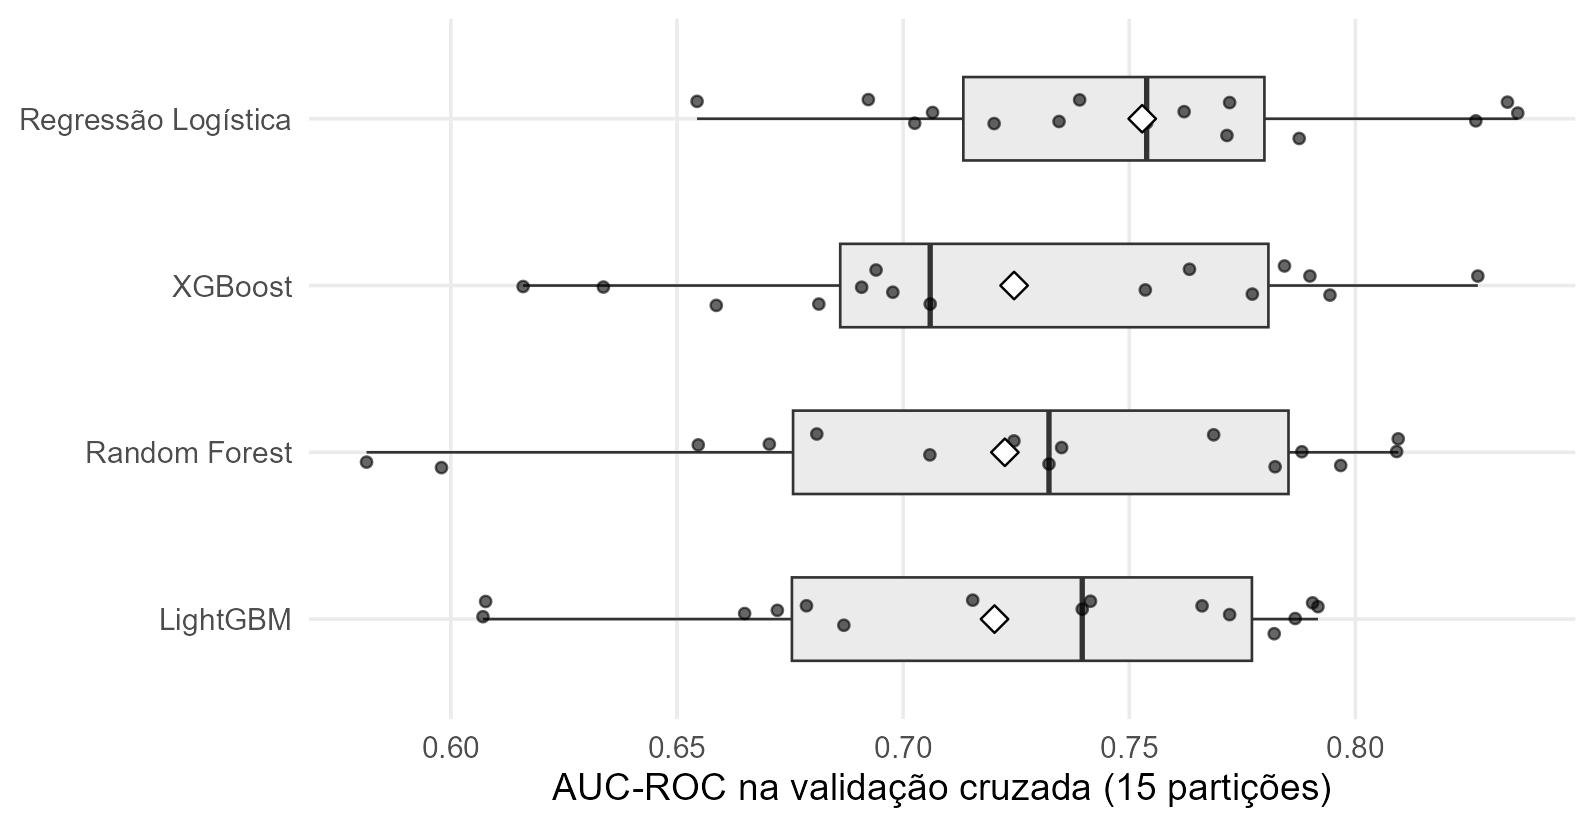
\includegraphics[width=0.75\textwidth]{figuras/cap5-resultados/cv_comparacao_modelos.png}
\caption{Distribuição da AUC-ROC nas 15 partições de validação. Cada ponto é uma partição, e o losango indica a média.}
\label{fig:res_cv}
\end{figure}

\subsection{Coeficientes da Regressão Logística}
\label{sec:res_coef_lr}

Sete variáveis tiveram coeficiente significativo a 5\% (Tabela~\ref{tab:res_coef_lr}). Idade, fosfatase alcalina e ALT aumentam a chance de doença, como esperado, mas as duas bilirrubinas e a AST, que estão entre as variáveis que mais diferem entre as classes, não foram significativas: como cada par correlacionado carrega quase a mesma informação, o modelo não consegue separar o efeito de cada variável \cite{Dormann2013Collinearity}. O mesmo explica os coeficientes das proteínas: \textit{Total\_Proteins} e \textit{Albumin} têm os maiores coeficientes, com sinais opostos (OR de 7,85 e 0,058), e \textit{AG\_Ratio} aumenta a chance de doença (OR 3,81), embora seja menor nos doentes. Por serem redundantes, os três coeficientes se compensam e só têm sentido em conjunto. Ou seja, mesmo o modelo ``interpretável'' exige cautela na leitura.

\begin{table}[htbp]
\centering
\caption{Coeficientes da Regressão Logística ajustada ao conjunto de treino (preditores padronizados).}
\label{tab:res_coef_lr}
\begin{tabular}{lrrr}
\hline
\textbf{Variável} & \textbf{Coeficiente} & \textbf{OR} & \textbf{$p$-valor} \\
\hline
Intercepto                  & 0,823  & 2,276 & $<0{,}001$ \\
Age                         & 0,317  & 1,374 & 0,002 \\
Gender                      & $-0{,}209$ & 0,811 & 0,037 \\
Total\_Bilirubin            & 0,278  & 1,321 & 0,646 \\
Direct\_Bilirubin           & 0,377  & 1,457 & 0,525 \\
Alkaline\_Phosphotase       & 0,428  & 1,534 & 0,004 \\
Alamine\_Aminotransferase   & 0,582  & 1,790 & 0,009 \\
Aspartate\_Aminotransferase & 0,280  & 1,322 & 0,202 \\
Total\_Proteins             & 2,060  & 7,849 & $<0{,}001$ \\
Albumin                     & $-2{,}851$ & 0,058 & $<0{,}001$ \\
AG\_Ratio                   & 1,338  & 3,809 & 0,002 \\
\hline
\multicolumn{4}{l}{\footnotesize OR: razão de chances para o aumento de um desvio-padrão.} \\
\multicolumn{4}{l}{\footnotesize \textit{Gender}: 1 = masculino, 0 = feminino, antes da padronização.} \\
\end{tabular}
\end{table}

% =============================================================================
\section{Avaliação no Conjunto de Teste}
\label{sec:res_teste}
% =============================================================================

\subsection{Métricas no Limiar Padrão}

No teste (Tabelas~\ref{tab:res_teste} e~\ref{tab:res_confusao}), o \textit{Random Forest} teve a maior AUC-ROC (0,787), seguido do LightGBM (0,761), do XGBoost (0,745) e da Regressão Logística (0,736), ordem praticamente inversa à da validação cruzada. Os intervalos de confiança se sobrepõem amplamente, com amplitude de cerca de 0,18, reflexo dos apenas 32 saudáveis no teste \cite{Hanley1982Meaning}. A acurácia (0,68 a 0,73) quase não supera a do classificador trivial (0,717) \cite{FAWCETT2006861}, e os modelos deixaram de identificar entre 19 e 25 dos 81 doentes, cerca de um em cada quatro.

\begin{table}[htbp]
\centering
\caption{Métricas no conjunto de teste ($n = 113$; 81 doentes e 32 saudáveis), com a regra de decisão padrão de cada modelo.}
\label{tab:res_teste}
\begin{tabular}{lccccc}
\hline
\textbf{Modelo} & \textbf{Acur.} & \textbf{Sens.} & \textbf{Espec.} & \textbf{Prec.} & \textbf{AUC-ROC [IC 95\%]} \\
\hline
Reg. Logística         & 0,681 & 0,728 & 0,563 & 0,808 & 0,736 [0,644; 0,829] \\
\textit{Random Forest} & 0,726 & 0,765 & 0,625 & 0,838 & 0,787 [0,703; 0,871] \\
XGBoost                & 0,717 & 0,716 & 0,719 & 0,866 & 0,745 [0,650; 0,840] \\
LightGBM               & 0,681 & 0,691 & 0,656 & 0,836 & 0,761 [0,671; 0,851] \\
\hline
\end{tabular}
\par\vspace{2pt}{\footnotesize IC: intervalo de confiança pelo método de DeLong. Classificador trivial (todos doentes): acurácia 0,717 e especificidade 0.}
\end{table}

\begin{table}[htbp]
\centering
\caption{Matrizes de confusão no conjunto de teste (regra de decisão padrão).}
\label{tab:res_confusao}
\begin{tabular}{lcccc}
\hline
\textbf{Modelo} & \textbf{VP} & \textbf{FN} & \textbf{VN} & \textbf{FP} \\
\hline
Regressão Logística    & 59 & 22 & 18 & 14 \\
\textit{Random Forest} & 62 & 19 & 20 & 12 \\
XGBoost                & 58 & 23 & 23 & 9 \\
LightGBM               & 56 & 25 & 21 & 11 \\
\hline
\multicolumn{5}{l}{\footnotesize VP e FN: entre os 81 doentes; VN e FP: entre os 32 saudáveis.} \\
\end{tabular}
\end{table}

Nenhuma das seis comparações pelo teste de DeLong foi significativa: a maior diferença, de 0,051 entre o \textit{Random Forest} e a Regressão Logística, teve $p = 0{,}090$ (0,541 após Bonferroni). Não há evidência de que algum modelo discrimine melhor que os outros, o que é coerente com revisões que não encontraram vantagem do aprendizado de máquina sobre a regressão logística em dados clínicos tabulares \cite{Christodoulou2019Systematic, Nusinovici2020Logistic}. Com 81 doentes e 32 saudáveis, o teste está abaixo dos cerca de 100 eventos e 100 não eventos sugeridos para validação \cite{Vergouwe2005Substantial}, e diferenças de 0,01 a 0,05 dificilmente seriam detectadas. As curvas ROC (Figura~\ref{fig:res_roc}) se cruzam várias vezes, sem que nenhum modelo domine os demais.

\begin{figure}[htbp]
\centering
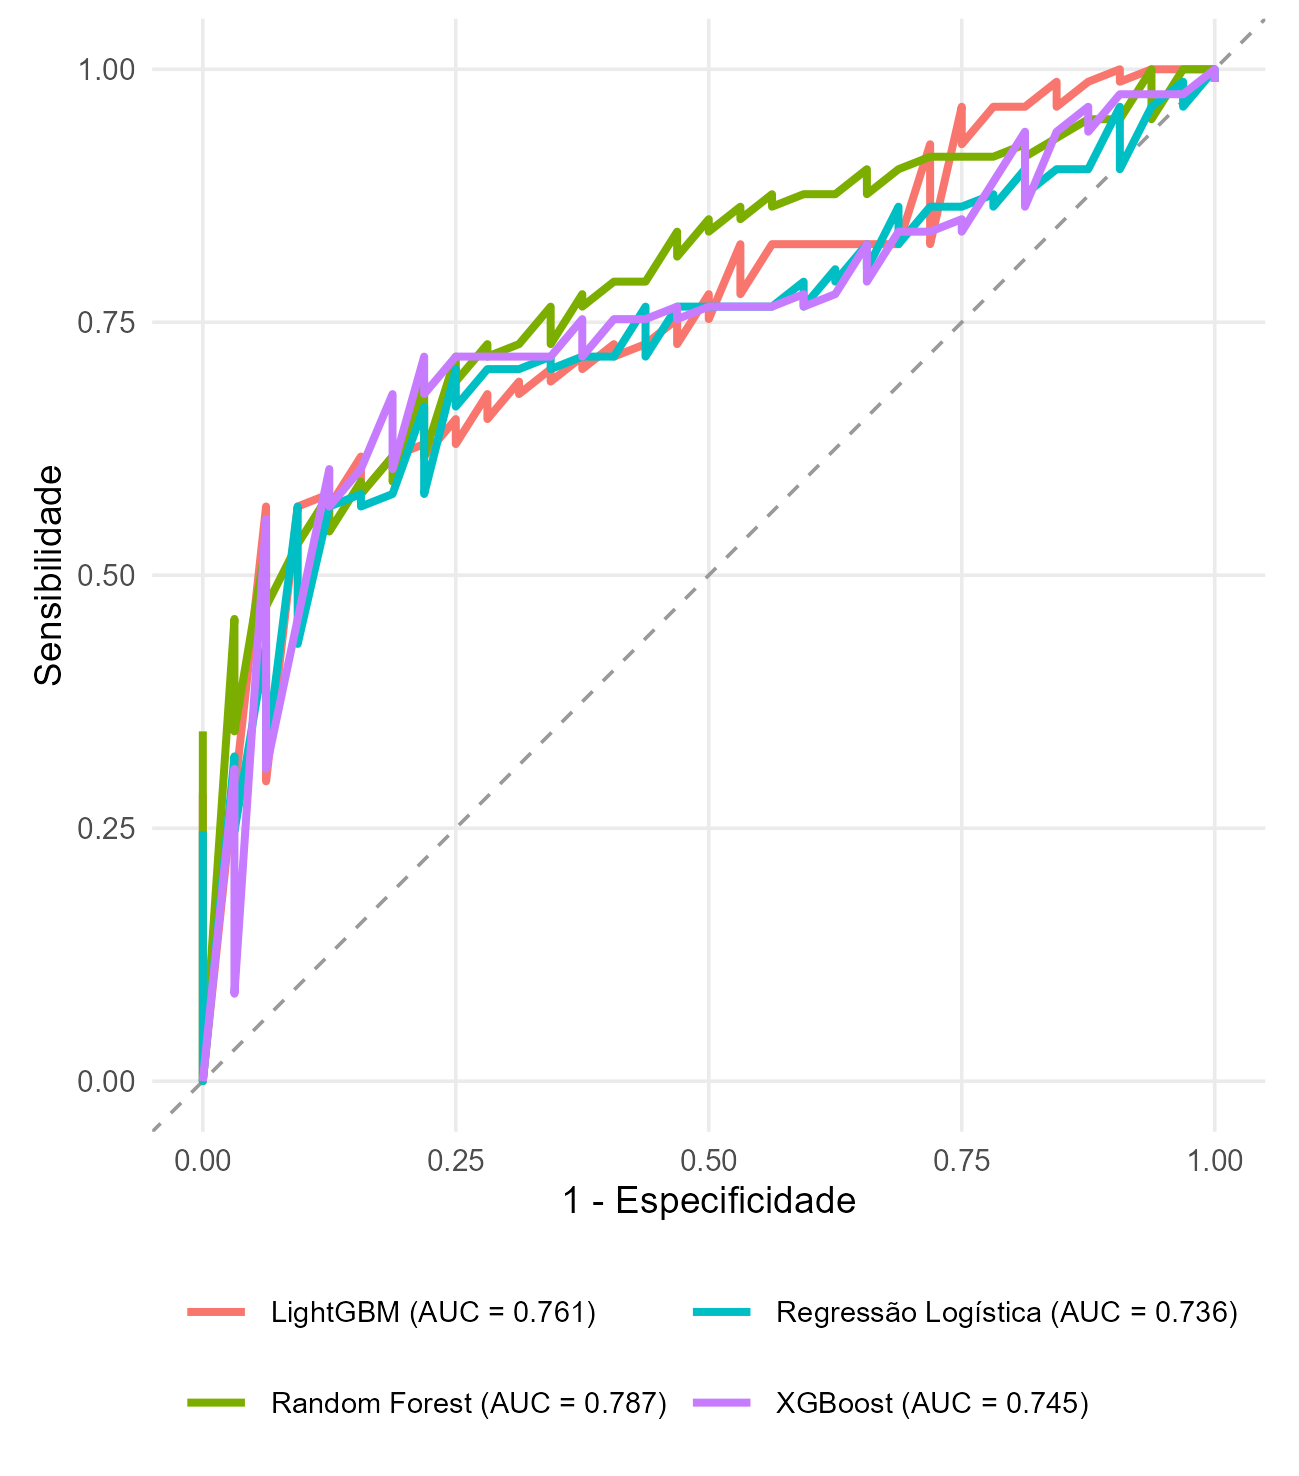
\includegraphics[width=0.6\textwidth]{figuras/cap5-resultados/roc_teste.png}
\caption{Curvas ROC dos quatro modelos no conjunto de teste. A diagonal tracejada representa um classificador aleatório.}
\label{fig:res_roc}
\end{figure}

\subsection{Análise do Limiar de Decisão}
\label{sec:res_limiar}

Os limiares clínicos ficaram entre 0,320 e 0,375 (Tabela~\ref{tab:res_limiares}). A meta de 90\% de sensibilidade se manteve no teste para a Regressão Logística, o \textit{Random Forest} e o LightGBM (73 de 81 doentes), mas não para o XGBoost (0,840). O custo é alto: a especificidade cai para 0,19 a 0,31 (só 6 a 10 dos 32 saudáveis reconhecidos), e a precisão fica apenas 2 a 5 pontos acima da prevalência de 0,717. No regime de triagem, portanto, os modelos acrescentam pouco em relação a encaminhar todos os pacientes para investigação, algo que a AUC sozinha não revela \cite{VanCalster2025Evaluation}.

\begin{table}[htbp]
\centering
\caption{Desempenho no conjunto de teste com o limiar clínico (sensibilidade $\geq$ 90\% na validação cruzada).}
\label{tab:res_limiares}
\begin{tabular}{lcccc}
\hline
\textbf{Modelo} & \textbf{Limiar} & \textbf{Sens.} & \textbf{Espec.} & \textbf{Prec.} \\
\hline
Reg. Logística         & 0,320 & 0,901 & 0,188 & 0,737 \\
\textit{Random Forest} & 0,375 & 0,901 & 0,313 & 0,768 \\
XGBoost                & 0,361 & 0,840 & 0,313 & 0,756 \\
LightGBM               & 0,360 & 0,901 & 0,281 & 0,760 \\
\hline
\end{tabular}
\end{table}

As probabilidades também não devem ser lidas como riscos reais: o SMOTE aumentou a proporção de saudáveis no treino, e a probabilidade média prevista pelo \textit{Random Forest} no teste (0,654) ficou abaixo da proporção real de doentes (0,717). A reamostragem tende a descalibrar os modelos sem melhorar a discriminação \cite{vandenGoorbergh2022Harm, Carriero2025Harms}; a calibração não foi avaliada neste trabalho.

% =============================================================================
\section{Avaliação Estratificada por Sexo}
\label{sec:res_sexo}
% =============================================================================

No teste, 17 das 32 mulheres (53,1\%) e 64 dos 81 homens (79,0\%) eram doentes. As diferenças de AUC entre os sexos foram pequenas, de $-0{,}043$ a $+0{,}019$ (Tabela~\ref{tab:res_sexo}), e os intervalos das mulheres têm o dobro da amplitude dos do conjunto completo. A taxa de falsos negativos foi maior entre as mulheres apenas no XGBoost (0,353 contra 0,266, diferença de cerca de dois pacientes) e menor nos outros três modelos. No limiar clínico, a meta de 90\% nem sempre foi atingida nos dois grupos: na Regressão Logística e no LightGBM, todas as mulheres doentes foram identificadas, mas os homens ficaram em 0,875.

\begin{table}[htbp]
\centering
\caption{Desempenho no conjunto de teste por sexo (F: 32 pacientes, 17 doentes; M: 81 pacientes, 64 doentes).}
\label{tab:res_sexo}
\small
\begin{tabular}{llcccccc}
\hline
 & & & \multicolumn{3}{c}{\textbf{Limiar padrão}} & \multicolumn{2}{c}{\textbf{Limiar clínico}} \\
\textbf{Modelo} & \textbf{Sexo} & \textbf{AUC-ROC [IC 95\%]} & \textbf{Sens.} & \textbf{Espec.} & \textbf{Taxa FN} & \textbf{Sens.} & \textbf{Espec.} \\
\hline
Reg. Logística         & F & 0,729 [0,546; 0,913] & 0,765 & 0,467 & 0,235 & 1,000 & 0,133 \\
                       & M & 0,748 [0,628; 0,868] & 0,719 & 0,647 & 0,281 & 0,875 & 0,235 \\
\textit{Random Forest} & F & 0,790 [0,619; 0,961] & 0,824 & 0,667 & 0,176 & 0,882 & 0,200 \\
                       & M & 0,781 [0,669; 0,894] & 0,766 & 0,588 & 0,234 & 0,906 & 0,412 \\
XGBoost                & F & 0,733 [0,551; 0,916] & 0,647 & 0,733 & 0,353 & 0,824 & 0,333 \\
                       & M & 0,743 [0,615; 0,870] & 0,734 & 0,706 & 0,266 & 0,844 & 0,294 \\
LightGBM               & F & 0,780 [0,618; 0,943] & 0,706 & 0,800 & 0,294 & 1,000 & 0,267 \\
                       & M & 0,737 [0,616; 0,858] & 0,688 & 0,529 & 0,313 & 0,875 & 0,294 \\
\hline
\multicolumn{8}{l}{\footnotesize Taxa FN: proporção de doentes classificados como saudáveis (1 $-$ sensibilidade).} \\
\end{tabular}
\end{table}

Esses resultados não reproduzem a disparidade relatada por \citeonline{investigatingbiashealth}, que encontraram taxas de falsos negativos cerca de 20 pontos maiores nas mulheres. A explicação mais simples é o tamanho da amostra: com 17 mulheres doentes, este trabalho não consegue confirmar nem descartar diferenças dessa magnitude, e a ausência de disparidade não deve ser lida como evidência de equidade \cite{Rajkomar2018Ensuring}.

% =============================================================================
\section{Interpretabilidade com SHAP}
\label{sec:res_shap}
% =============================================================================

O valor base, previsão média no teste a partir da qual as contribuições são somadas, foi de 0,167 log-odds no XGBoost (probabilidade de cerca de 0,54), 0,304 no LightGBM (cerca de 0,58) e 0,654 em probabilidade no \textit{Random Forest}.

\subsection{Importância Global}
\label{sec:res_shap_global}

Os três modelos concordam que as bilirrubinas, a fosfatase alcalina e as aminotransferases são as variáveis mais relevantes e que o sexo é pouco relevante, mas distribuem a importância de formas muito diferentes (Tabela~\ref{tab:res_shap_imp}).

\begin{table}[htbp]
\centering
\caption{Importância SHAP global (média dos valores SHAP absolutos no teste): posição no ranking e participação percentual na importância total.}
\label{tab:res_shap_imp}
\begin{tabular}{lcccccc}
\hline
 & \multicolumn{2}{c}{\textbf{XGBoost}} & \multicolumn{2}{c}{\textbf{LightGBM}} & \multicolumn{2}{c}{\textbf{\textit{Random Forest}}} \\
\textbf{Variável} & \textbf{Pos.} & \textbf{\%} & \textbf{Pos.} & \textbf{\%} & \textbf{Pos.} & \textbf{\%} \\
\hline
Total\_Bilirubin            & 1     & 37,6 & 4  & 16,5 & 3  & 13,8 \\
Alkaline\_Phosphotase       & 2     & 26,4 & 1  & 23,0 & 1  & 18,4 \\
Total\_Proteins             & 3     & 8,5  & 9  & 0,7  & 9  & 4,9 \\
Aspartate\_Aminotransferase & 4     & 8,1  & 3  & 16,8 & 5  & 11,8 \\
Age                         & 5     & 7,9  & 6  & 7,3  & 6  & 8,1 \\
AG\_Ratio                   & 6     & 5,8  & 7  & 5,4  & 7  & 7,3 \\
Alamine\_Aminotransferase   & 7     & 5,6  & 5  & 9,1  & 4  & 12,0 \\
Direct\_Bilirubin           & 8--10 & 0,0  & 2  & 19,2 & 2  & 14,7 \\
Albumin                     & 8--10 & 0,0  & 8  & 2,1  & 8  & 6,0 \\
Gender                      & 8--10 & 0,0  & 10 & 0,0  & 10 & 3,1 \\
\hline
\multicolumn{7}{l}{\footnotesize Variáveis não utilizadas por um modelo têm importância nula e empatam nas últimas posições.} \\
\end{tabular}
\end{table}

No XGBoost, a importância é concentrada: bilirrubina total e fosfatase alcalina somam 64\%, e \textit{Direct\_Bilirubin}, \textit{Albumin} e \textit{Gender} têm importância nula porque não aparecem em nenhuma árvore. Com poucas árvores e forte regularização (Tabela~\ref{tab:res_hiper}), o modelo faz poucas divisões e, entre variáveis redundantes, usa apenas uma: a bilirrubina total em vez da direta, e \textit{Total\_Proteins} e \textit{AG\_Ratio}, que juntas determinam a albumina. No \textit{Random Forest}, ao contrário, a importância é distribuída: as cinco primeiras variáveis têm entre 11,8\% e 18,4\%. Com \texttt{mtry} = 1, o modelo alterna entre variáveis correlacionadas e divide o crédito entre elas, comportamento conhecido tanto para o \textit{Random Forest} \cite{Strobl2008Conditional} quanto para o SHAP \cite{Aas2021Explaining}. O LightGBM, embora seja de \textit{boosting} como o XGBoost, se parece mais com o \textit{Random Forest}: suas muitas árvores pequenas acabam usando as duas variáveis de cada par, mas ele praticamente ignora as proteínas e não usa \textit{Gender}.

As cinco variáveis mais importantes no \textit{Random Forest} e no LightGBM são exatamente as cinco cuja média mais difere entre as classes (Tabela~\ref{tab:medias_classe}). Já no XGBoost, \textit{Total\_Proteins}, que quase não difere entre as classes, ficou em terceiro, o que indica um papel condicional às demais variáveis. Cada retrato descreve corretamente o seu modelo, mas, juntos, mostram que a importância de uma variável depende também do algoritmo e dos hiperparâmetros.

\subsection{Direção e Forma dos Efeitos}
\label{sec:res_shap_direcao}

Os \textit{beeswarms} (Figura~\ref{fig:res_beeswarm}) e as correlações entre o valor e o SHAP de cada variável (Tabela~\ref{tab:res_direcao}) mostram efeitos no mesmo sentido nos três modelos: valores altos de bilirrubinas, fosfatase alcalina, aminotransferases e idade aumentam a previsão de doença, e valores altos de \textit{AG\_Ratio} (e de albumina, no \textit{Random Forest}) a reduzem. Esses sentidos são coerentes com a clínica \cite{Kwo2016ACG, Trebicka2025Controversies}, o que não prova causalidade, mas indica que os modelos não se apoiam em padrões espúrios.

\begin{figure}[htbp]
\centering
\begin{minipage}{0.49\textwidth}
\centering
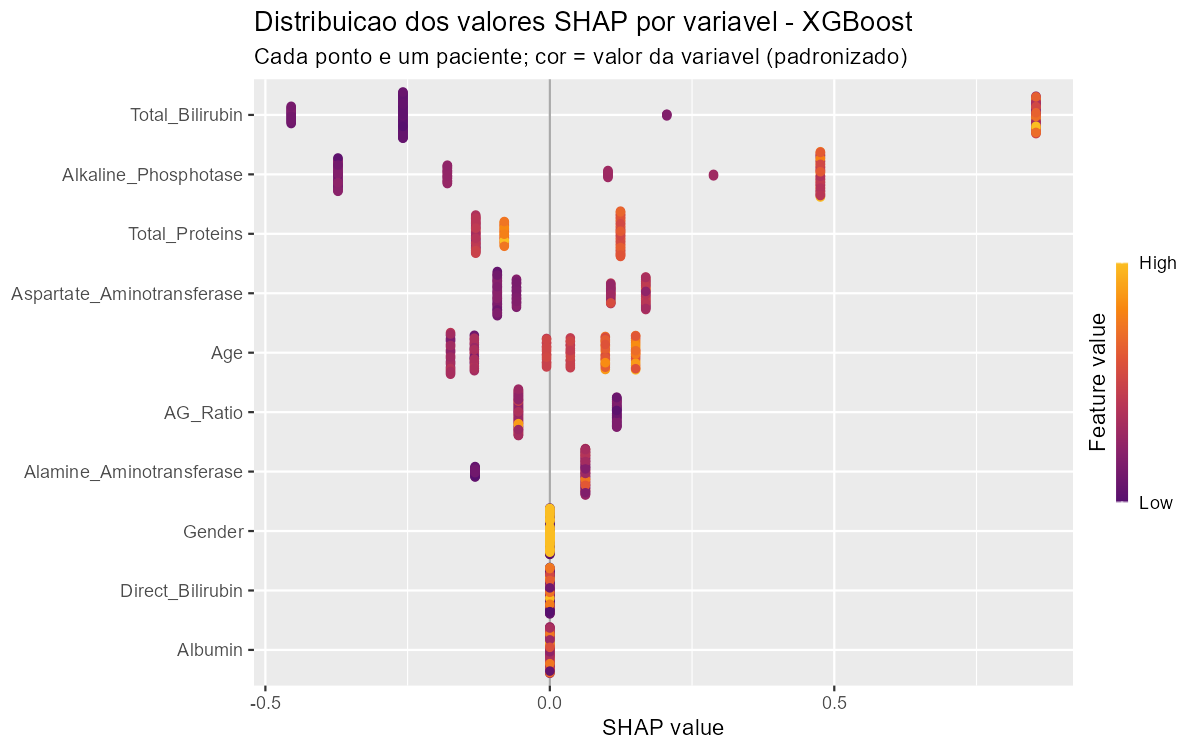
\includegraphics[width=\textwidth]{figuras/cap5-resultados/shap_beeswarm_xgb.png}\\
\small (a) XGBoost
\end{minipage}
\hfill
\begin{minipage}{0.49\textwidth}
\centering
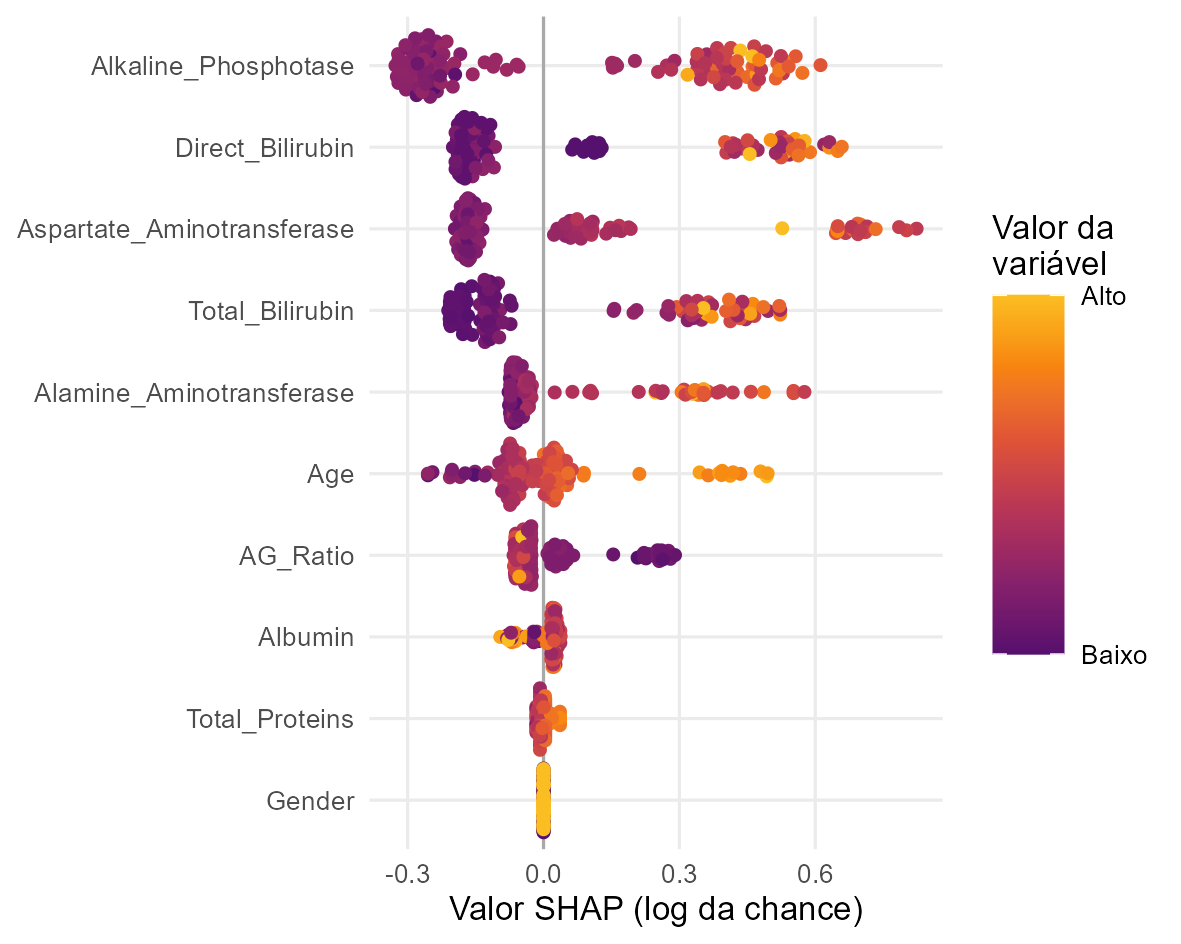
\includegraphics[width=\textwidth]{figuras/cap5-resultados/shap_beeswarm_lgb.png}\\
\small (b) LightGBM
\end{minipage}

\vspace{0.3cm}

\begin{minipage}{0.49\textwidth}
\centering
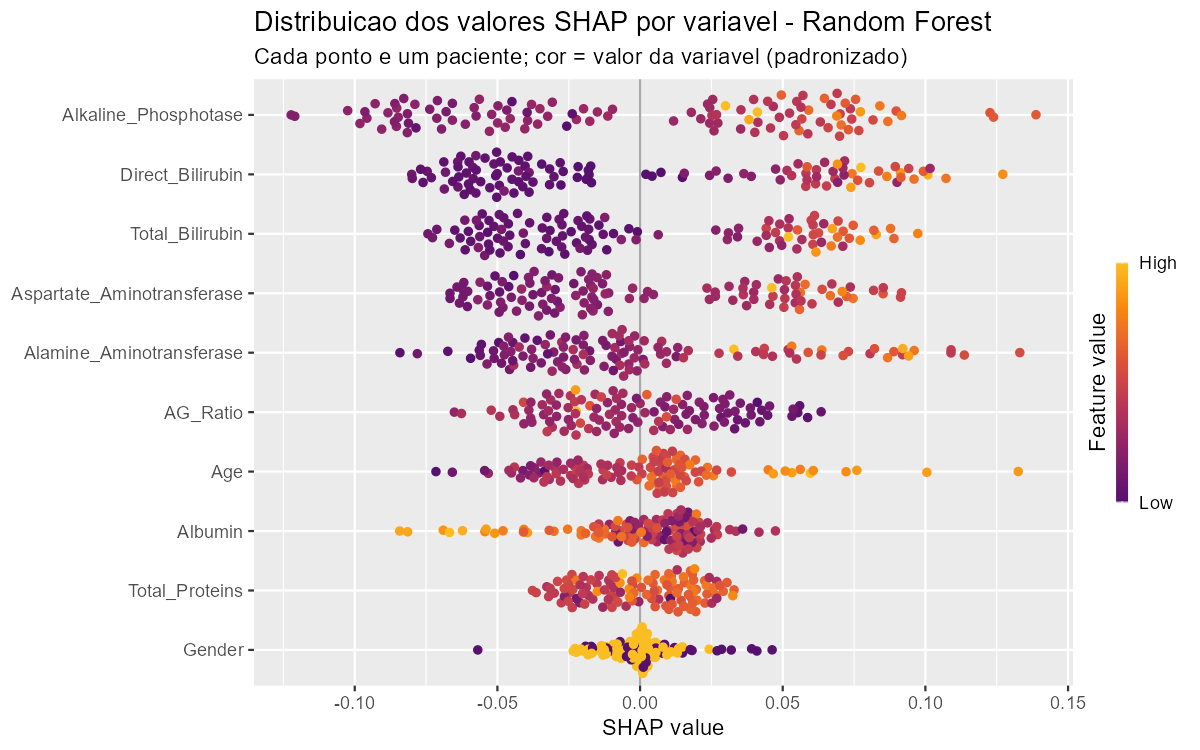
\includegraphics[width=\textwidth]{figuras/cap5-resultados/shap_beeswarm_rf.png}\\
\small (c) \textit{Random Forest}
\end{minipage}
\caption{Valores SHAP por variável no conjunto de teste. Cada ponto é um paciente, colorido do menor ao maior valor da variável; pontos à direita do zero aumentam a previsão de doença.}
\label{fig:res_beeswarm}
\end{figure}

\begin{table}[htbp]
\centering
\caption{Correlação de Pearson entre o valor de cada variável e seu valor SHAP no conjunto de teste.}
\label{tab:res_direcao}
\begin{tabular}{lccc}
\hline
\textbf{Variável} & \textbf{XGBoost} & \textbf{LightGBM} & \textbf{\textit{Random Forest}} \\
\hline
Age                         & 0,860      & 0,868      & 0,894 \\
Total\_Bilirubin            & 0,807      & 0,864      & 0,855 \\
Direct\_Bilirubin           & ---        & 0,819      & 0,818 \\
Alkaline\_Phosphotase       & 0,810      & 0,816      & 0,754 \\
Alamine\_Aminotransferase   & 0,531      & 0,791      & 0,841 \\
Aspartate\_Aminotransferase & 0,717      & 0,874      & 0,824 \\
Total\_Proteins             & 0,360      & 0,770      & 0,425 \\
Albumin                     & ---        & $-0{,}046$ & $-0{,}737$ \\
AG\_Ratio                   & $-0{,}669$ & $-0{,}668$ & $-0{,}572$ \\
Gender                      & ---        & ---        & $-0{,}140$ \\
\hline
\multicolumn{4}{l}{\footnotesize ---: variável não utilizada pelo modelo (valores SHAP constantes).} \\
\end{tabular}
\end{table}

A forma dos efeitos difere (Figura~\ref{fig:res_dependencia}). No XGBoost, cada variável participa de poucas divisões, e o efeito é em degraus: na bilirrubina total, pacientes a partir de cerca de 1,8~mg/dL recebem $+0{,}86$ log-odds, e um paciente com 1,6~mg/dL já recebe $-0{,}45$. Em \textit{Total\_Proteins}, o efeito não é monotônico (valores intermediários aumentam a previsão), o que explica sua correlação fraca e provavelmente funciona como substituto da albumina, mas é difícil de traduzir em regra clínica. No LightGBM e no \textit{Random Forest}, cuja variável mais importante é a fosfatase alcalina, a curva tem forma de ``S'', quase um degrau no LightGBM e mais gradual no \textit{Random Forest}.

\begin{figure}[htbp]
\centering
\begin{minipage}{0.49\textwidth}
\centering
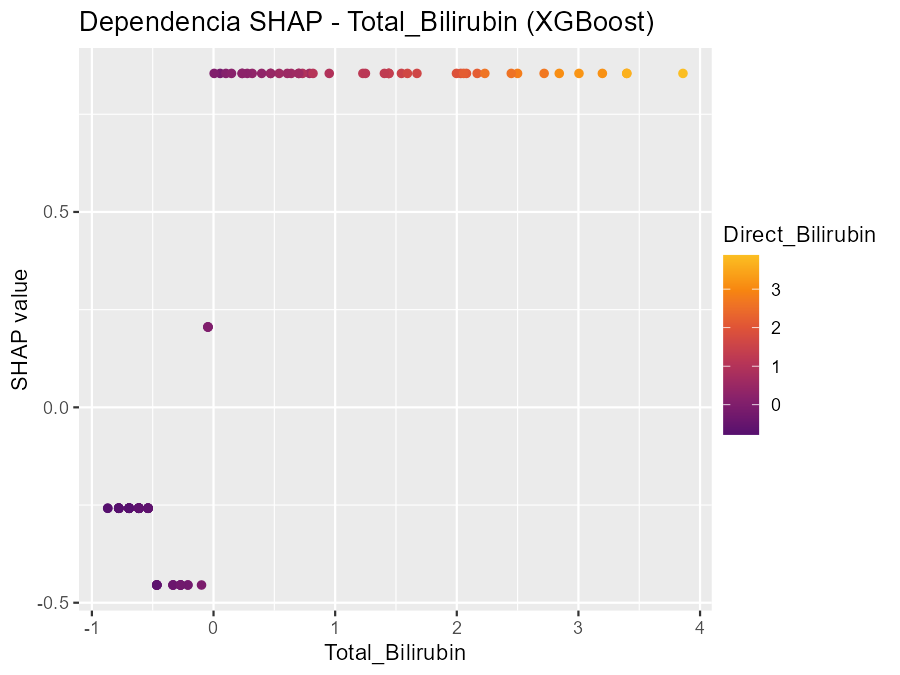
\includegraphics[width=\textwidth]{figuras/cap5-resultados/shap_dependencia_xgb_Total_Bilirubin.png}\\
\small (a) XGBoost: \textit{Total\_Bilirubin}
\end{minipage}
\hfill
\begin{minipage}{0.49\textwidth}
\centering
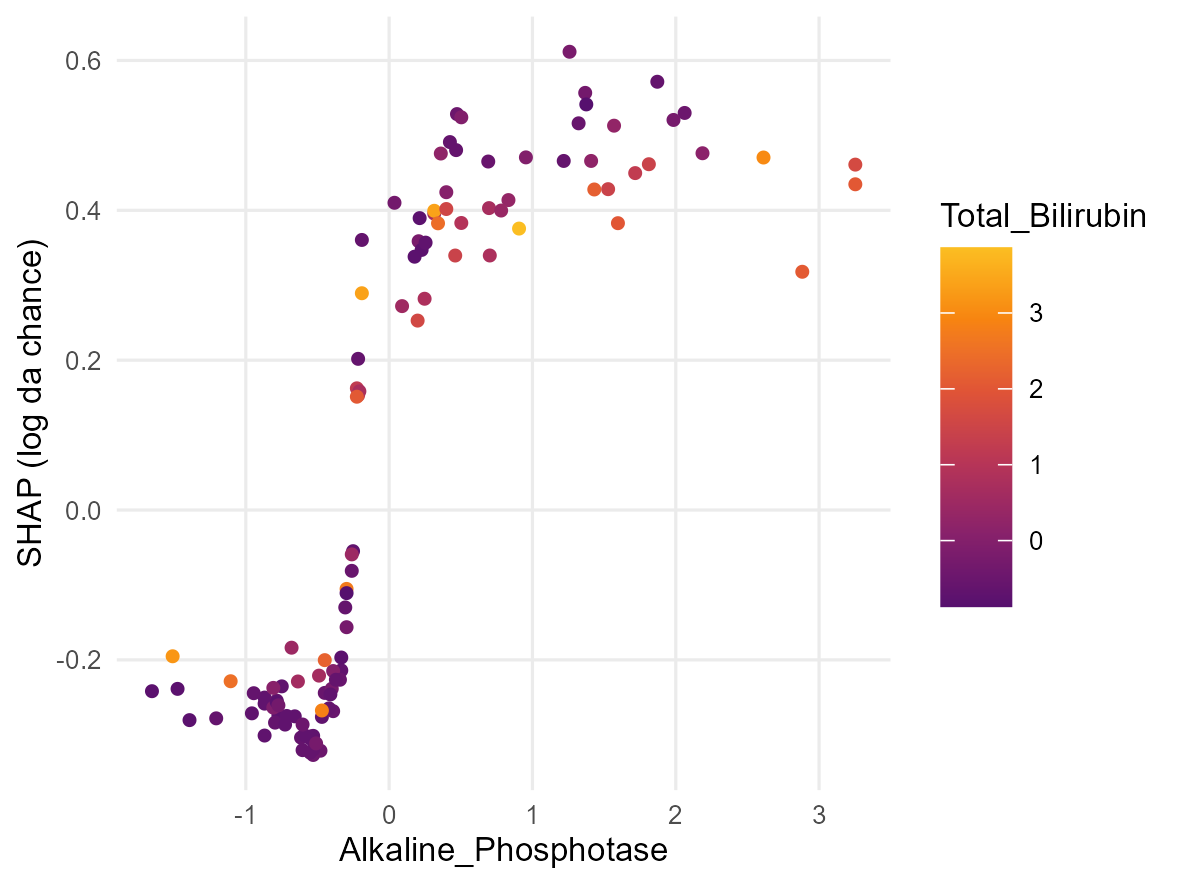
\includegraphics[width=\textwidth]{figuras/cap5-resultados/shap_dependencia_lgb_Alkaline_Phosphotase.png}\\
\small (b) LightGBM: \textit{Alkaline\_Phosphotase}
\end{minipage}

\vspace{0.3cm}

\begin{minipage}{0.49\textwidth}
\centering
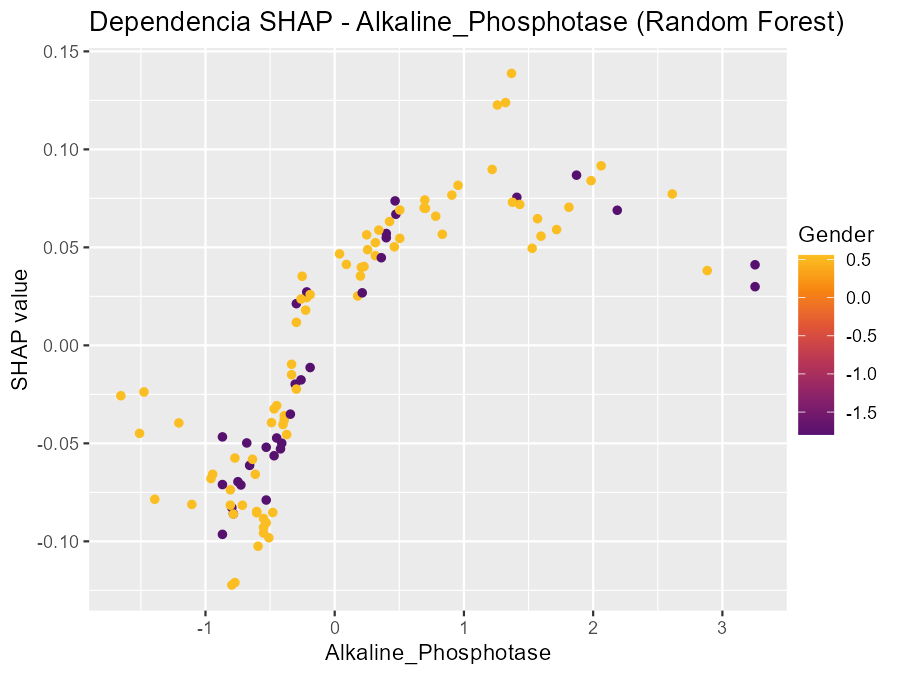
\includegraphics[width=\textwidth]{figuras/cap5-resultados/shap_dependencia_rf_Alkaline_Phosphotase.png}\\
\small (c) \textit{Random Forest}: \textit{Alkaline\_Phosphotase}
\end{minipage}
\caption{Gráficos de dependência SHAP da variável mais importante de cada modelo (eixo horizontal na escala padronizada).}
\label{fig:res_dependencia}
\end{figure}

\subsection{Explicações Locais}
\label{sec:res_shap_local}

Nos verdadeiros positivos de maior confiança, os três modelos se apoiaram nos mesmos exames, muito acima das medianas da base: por exemplo, no LightGBM, um homem de 66 anos com AST de 4.929~IU/L (o maior valor da base) recebeu probabilidade de 0,92. Os valores dos exames citados nesta seção foram convertidos para as unidades originais.

Os falsos negativos de pior erro (Figura~\ref{fig:res_waterfall_fn}) são mais reveladores. No XGBoost, um homem de 35 anos recebeu probabilidade de apenas 0,224: sua bilirrubina total (1,6~mg/dL) ficou logo abaixo do degrau de 1,8~mg/dL e gerou a maior contribuição para ``saudável'', enquanto sua albumina baixa (2,5~g/dL), um possível sinal de doença, não teve efeito porque o modelo não usa essa variável. No LightGBM, um homem de 30 anos (probabilidade de 0,334) também tinha albumina (2,3~g/dL) e proteínas totais (4,6~g/dL) baixas, sinais que o modelo praticamente ignora. Esses casos mostram que um modelo que descarta variáveis \emph{em média} pode descartar justamente a informação decisiva para um paciente.

\begin{figure}[htbp]
\centering
\begin{minipage}{0.49\textwidth}
\centering
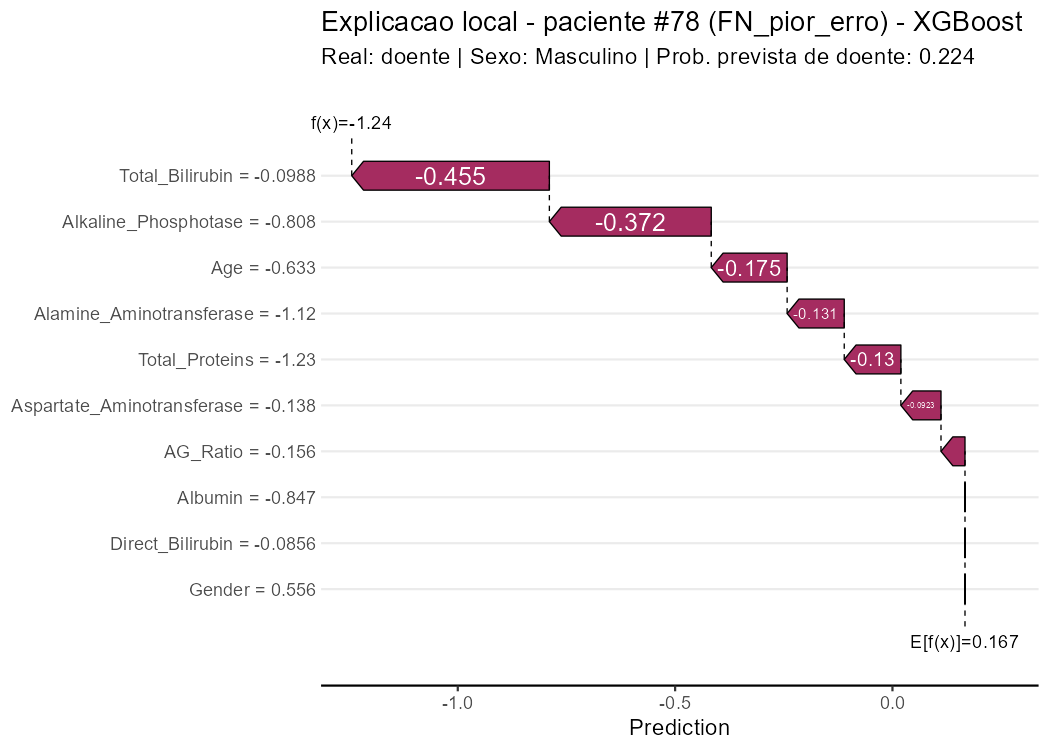
\includegraphics[width=\textwidth]{figuras/cap5-resultados/shap_waterfall_xgb_FN_pior_erro.png}\\
\small (a) XGBoost
\end{minipage}
\hfill
\begin{minipage}{0.49\textwidth}
\centering
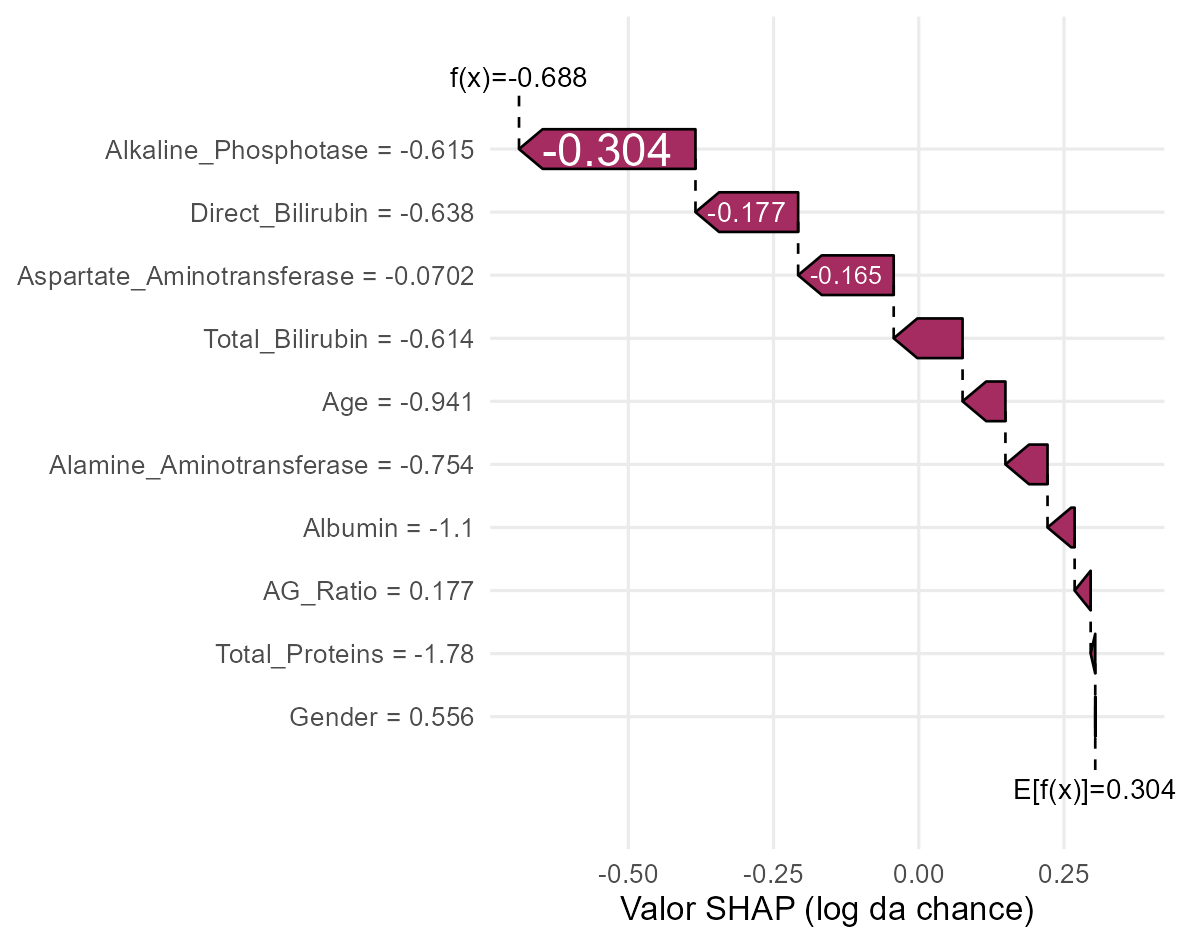
\includegraphics[width=\textwidth]{figuras/cap5-resultados/shap_waterfall_lgb_FN_pior_erro.png}\\
\small (b) LightGBM
\end{minipage}

\vspace{0.3cm}

\begin{minipage}{0.49\textwidth}
\centering
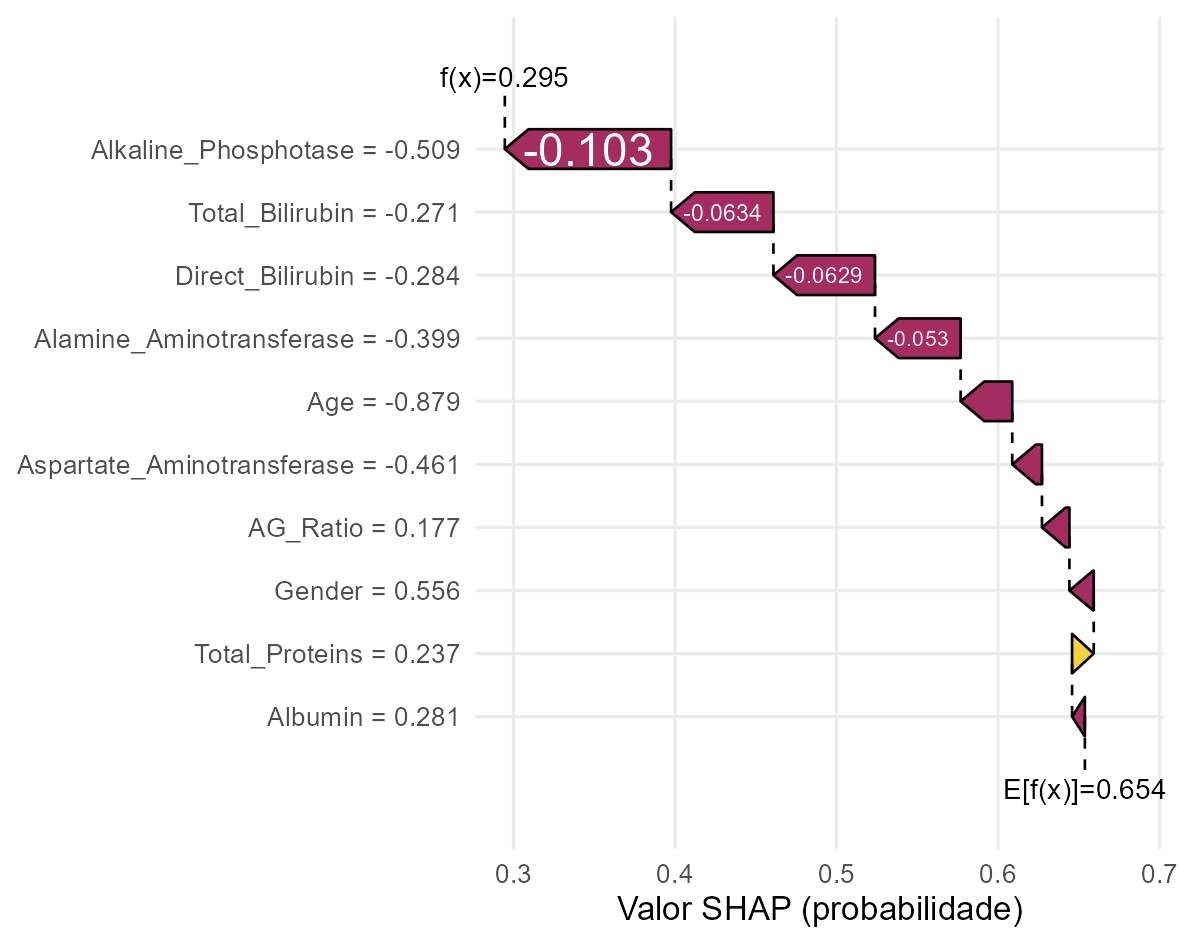
\includegraphics[width=\textwidth]{figuras/cap5-resultados/shap_waterfall_rf_FN_pior_erro.png}\\
\small (c) \textit{Random Forest}
\end{minipage}
\caption{Explicações locais dos falsos negativos de pior erro (pacientes doentes classificados com maior confiança como saudáveis).}
\label{fig:res_waterfall_fn}
\end{figure}

No \textit{Random Forest}, o falso negativo de pior erro (homem de 31 anos, probabilidade de 0,248) tinha exames compatíveis com os de um paciente saudável, como ALT de 29~IU/L, abaixo do limite de 42~IU/L proposto para homens por \citeonline{Valenti2021Definition}. Aqui, o erro parece vir da própria informação disponível, já que a doença hepática pode existir com exames normais \cite{Lominadze2018Misconception}. As explicações locais permitem, assim, distinguir erros causados pelas escolhas do modelo de erros que nenhum modelo baseado nesses atributos evitaria. Como os valores SHAP do \textit{Random Forest} são estimados por amostragem, sua soma não reproduz exatamente a previsão (0,295 contra 0,248 nesse paciente), e contribuições pequenas devem ser lidas com cautela.

\subsection{Auditoria de Viés por Sexo}
\label{sec:res_shap_sexo}

A importância das variáveis foi muito semelhante entre os sexos (Figura~\ref{fig:res_shap_sexo}): a correlação de Spearman entre os rankings de homens e mulheres foi de 0,988 nos três modelos, com apenas trocas entre variáveis vizinhas. O XGBoost e o LightGBM não usam \textit{Gender}. No \textit{Random Forest}, \textit{Gender} é a variável menos importante, e sua contribuição média foi de $+0{,}0030$ nas mulheres e $-0{,}0015$ nos homens (Figura~\ref{fig:res_shap_gender}), no mesmo sentido do coeficiente da Regressão Logística, mas menor que meio ponto percentual. A auditoria não encontrou, portanto, indício de que os modelos usem o sexo como atalho ou se apoiem em variáveis diferentes para cada grupo, com as mesmas limitações de tamanho amostral já discutidas.

\begin{figure}[htbp]
\centering
\begin{minipage}{0.49\textwidth}
\centering
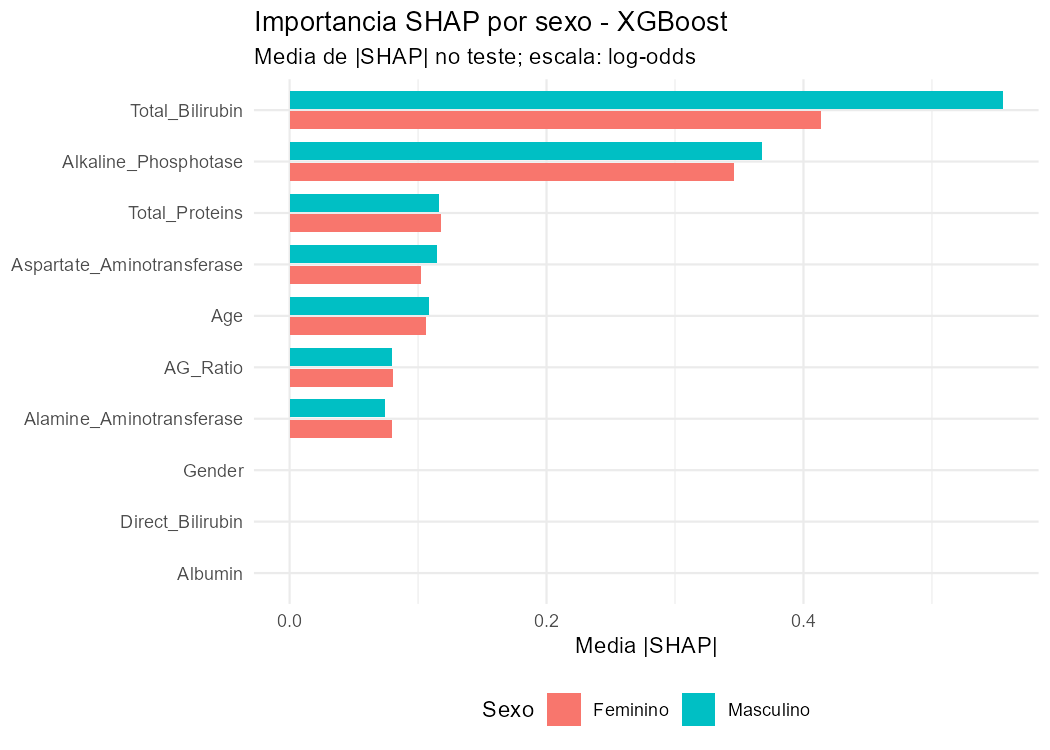
\includegraphics[width=\textwidth]{figuras/cap5-resultados/shap_importancia_por_sexo_xgb.png}\\
\small (a) XGBoost
\end{minipage}
\hfill
\begin{minipage}{0.49\textwidth}
\centering
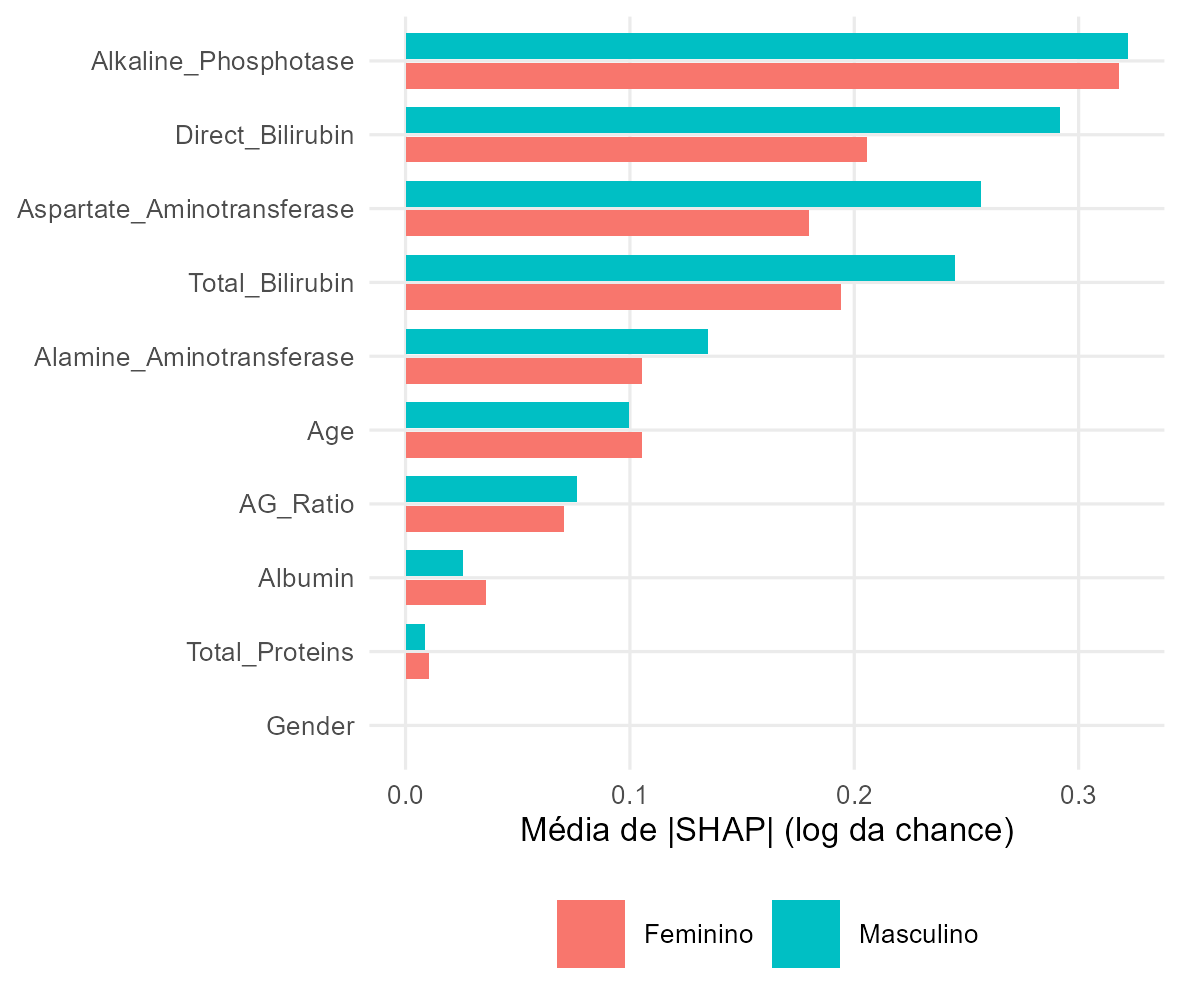
\includegraphics[width=\textwidth]{figuras/cap5-resultados/shap_importancia_por_sexo_lgb.png}\\
\small (b) LightGBM
\end{minipage}

\vspace{0.3cm}

\begin{minipage}{0.49\textwidth}
\centering
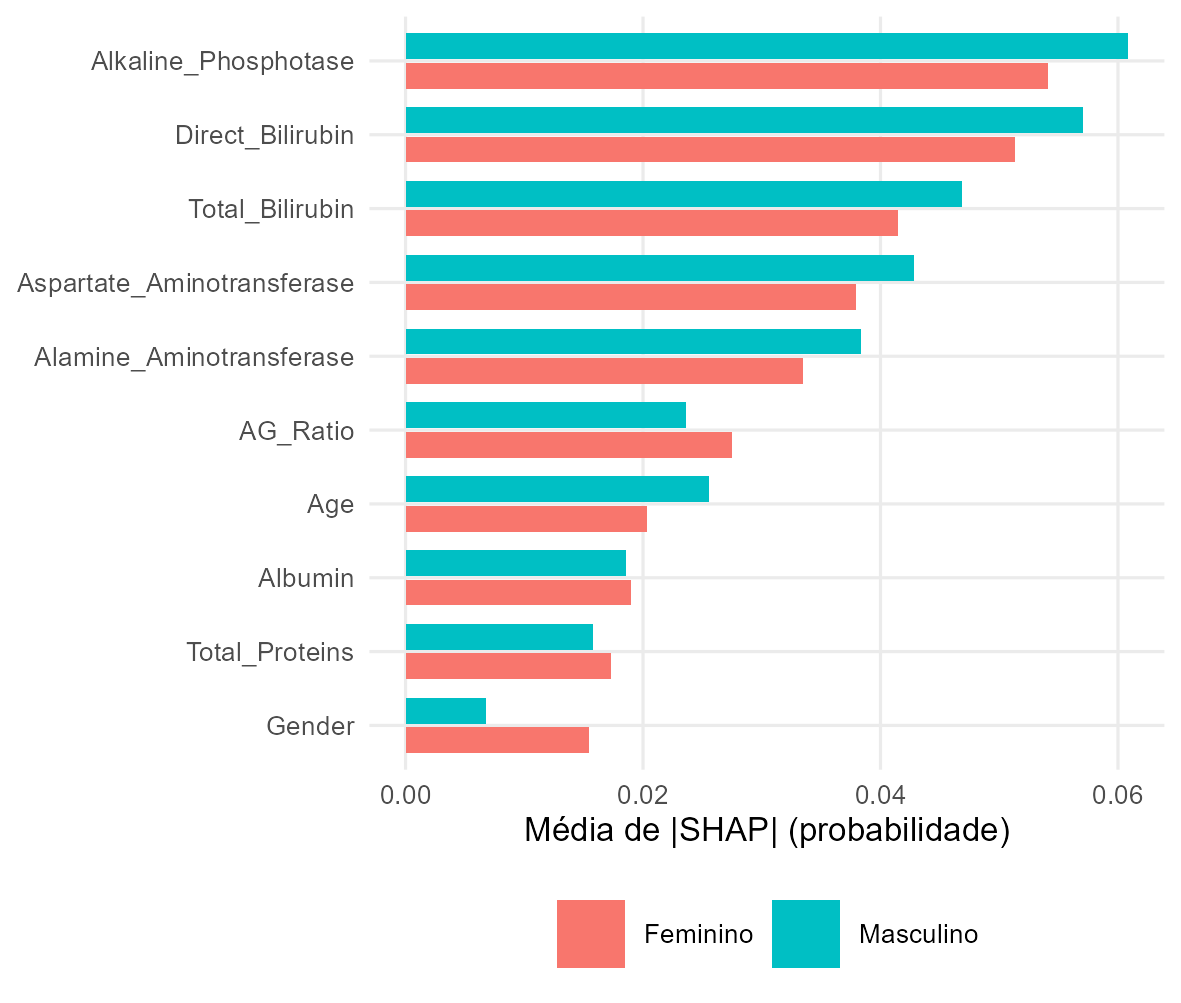
\includegraphics[width=\textwidth]{figuras/cap5-resultados/shap_importancia_por_sexo_rf.png}\\
\small (c) \textit{Random Forest}
\end{minipage}
\caption{Importância SHAP global calculada separadamente para os pacientes de cada sexo no conjunto de teste.}
\label{fig:res_shap_sexo}
\end{figure}

\begin{figure}[htbp]
\centering
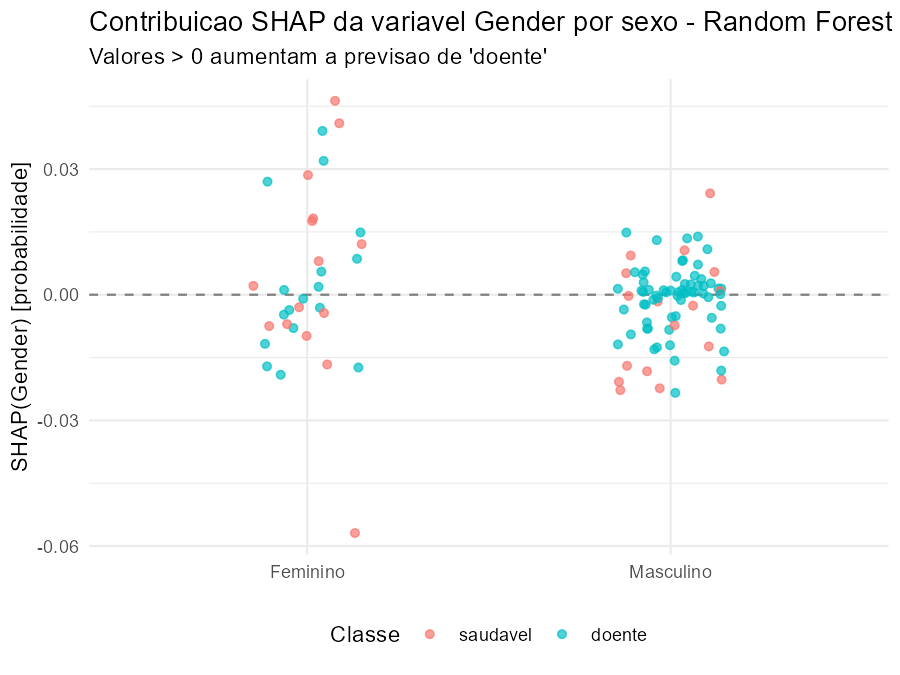
\includegraphics[width=0.55\textwidth]{figuras/cap5-resultados/shap_gender_por_sexo_rf.png}
\caption{Contribuição SHAP da variável \textit{Gender} no \textit{Random Forest}, por sexo e classe real. Valores positivos aumentam a probabilidade prevista de doença.}
\label{fig:res_shap_gender}
\end{figure}

\subsection{Comparação das Importâncias entre os Modelos}
\label{sec:res_comparacao_importancias}

Os rankings do LightGBM e do \textit{Random Forest} foram quase idênticos ($\rho = 0{,}96$), embora um use \textit{boosting} e o outro \textit{bagging}; o do XGBoost concordou pouco com ambos ($\rho = 0{,}36$), e o da Regressão Logística teve correlação negativa com todos (Tabela~\ref{tab:res_rankings}). O ranking da Regressão Logística é dominado pelas proteínas, cujos coeficientes são grandes porque se compensam (Seção~\ref{sec:res_coef_lr}), e não por serem as mais informativas \cite{Dormann2013Collinearity}. O XGBoost se afasta dos outros dois porque escolheu uma variável de cada par redundante, enquanto os demais dividiram o crédito. A distribuição da importância depende, portanto, mais da configuração do modelo do que da estratégia de \textit{ensemble}.

\begin{table}[htbp]
\centering
\caption{Posição de cada variável nos quatro rankings de importância (1 = mais importante).}
\label{tab:res_rankings}
\begin{tabular}{lcccc}
\hline
 & \multicolumn{3}{c}{\textbf{SHAP}} & \textbf{$|$Coef.$|$} \\
\textbf{Variável} & \textbf{XGB} & \textbf{LGB} & \textbf{RF} & \textbf{RL} \\
\hline
Total\_Bilirubin            & 1 & 4  & 3  & 9 \\
Alkaline\_Phosphotase       & 2 & 1  & 1  & 5 \\
Total\_Proteins             & 3 & 9  & 9  & 2 \\
Aspartate\_Aminotransferase & 4 & 3  & 5  & 8 \\
Age                         & 5 & 6  & 6  & 7 \\
AG\_Ratio                   & 6 & 7  & 7  & 3 \\
Alamine\_Aminotransferase   & 7 & 5  & 4  & 4 \\
Direct\_Bilirubin           & 9 & 2  & 2  & 6 \\
Albumin                     & 9 & 8  & 8  & 1 \\
Gender                      & 9 & 10 & 10 & 10 \\
\hline
\multicolumn{5}{l}{\footnotesize XGB: XGBoost; LGB: LightGBM; RF: \textit{Random Forest}; RL: Regressão Logística.} \\
\multicolumn{5}{l}{\footnotesize Empates recebem o posto médio. Spearman: XGB--LGB $= 0{,}362$; XGB--RF $= 0{,}362$;} \\
\multicolumn{5}{l}{\footnotesize LGB--RF $= 0{,}964$; XGB--RL $= -0{,}141$; LGB--RL $= -0{,}200$; RF--RL $= -0{,}164$.} \\
\end{tabular}
\end{table}

Alguns resultados se repetem em todos os modelos: uma das bilirrubinas e a fosfatase alcalina estão sempre entre as mais importantes nos três \textit{ensembles}, e \textit{Gender} fica nas últimas posições nos quatro rankings. São esses resultados estáveis, e não a posição exata de cada variável, que podem ser afirmados com segurança. Modelos com desempenho estatisticamente indistinguível podem oferecer explicações bem diferentes dos mesmos dados, o chamado efeito Rashomon \cite{Biecek2024Performance}, e a interpretação de um único modelo não deve ser tomada como descrição definitiva da relação entre os exames e a doença.

% =============================================================================
\section{Síntese dos Resultados}
\label{sec:res_sintese}
% =============================================================================

\begin{enumerate}
    \item \textit{Desempenho}: nenhum \textit{ensemble} superou a Regressão Logística de forma significativa; as AUCs (0,74 a 0,79) indicam discriminação moderada, com intervalos largos.
    \item \textit{Limiar}: exigir 90\% de sensibilidade reduz a especificidade a 0,19--0,31, e os modelos acrescentam pouco à triagem de todos os pacientes.
    \item \textit{Sexo}: não houve disparidade consistente de desempenho nem de uso das variáveis, mas o subgrupo feminino é pequeno demais para descartá-la.
    \item \textit{Interpretabilidade}: os efeitos estimados pelo SHAP são coerentes com a clínica, mas a importância das variáveis depende do modelo e dos hiperparâmetros, sobretudo entre variáveis correlacionadas.
    \item \textit{Explicações locais}: os falsos negativos permitiram distinguir erros causados pelo modelo (descarte das proteínas no XGBoost e no LightGBM) de erros inevitáveis com esses atributos.
\end{enumerate}

Como limitações, o teste é pequeno e vem de uma única divisão \cite{Vergouwe2005Substantial}, a calibração e a utilidade clínica não foram avaliadas \cite{Vickers2006Decision}, e os valores SHAP do \textit{Random Forest} são aproximações. Esses pontos são retomados na Conclusão.

\chapter*{CONCLUSÃO} 
\addcontentsline{toc}{chapter}{CONCLUSÃO}
\thispagestyle{plain}

Nesta seção são descritas claramente as conclusões retiradas das
discussões e dos experimentos realizados no decorrer da pesquisa, e finalizada a parte textual do trabalho. A Conclusão deve dialogar com a Introdução, melhor dizendo, apontar ou sugerir questões e problemas decorrentes do assunto apresentado, mostrando se os objetivos foram atingidos ou não e se as hipóteses foram ou não confirmadas. Também deve trazer recomendações e uma breve explanação sobre trabalhos futuros.

%MAIS DICAS
%
%Sua conclusão pode apresentar uma estrutura como a seguinte:
%Este trabalho apresentou .... De uma maneira geral a 
%
%A primeira etapa foi ..
%
%
%Para a segunda etapa, que é a ... O algoritmo que separa em regiões foi adaptado ao processamento morfológico resultando em .. 
%
%A terceira e última etapa, que é a ... 
%
%
%
%
%Portanto, as principais contribuições do presente trabalho são: ...
%
%
%E como trabalhos futuros, será implementado um novo método baseado em \textit{roughness index 3D}; serão desenvolvidas redes convolucionais para ..            %inserindo a conclusão
%---------------------------------------------------------------------
% BIBLIOGRAFIA
%		Edite o arquivo bibliografia, apenas acrescentando 
%		novas obras, não é necessário remover nada pois o 
%		latex insere somente as obras referenciadas. Ele também
%		ordena tudo!!! A configuração padrão deste modelo é a 
%		ordem alfabética (uma alternativa seria a ordem de 
%		citação no texto)
%       Para facilitar a confecção da bibliografia recomenda-se o 
% 		uso de aplicativos como Mendeley que gera arquivos .bib
%
%		IMPORTANTE: é necessário atualizar o documento todas 
%		as vezes que inserir um novo item na bibliografia. 
%		Procure o manual do seu editor para Saber como proceder.
%		Exemplo: TeXMaker 3.5.2
%		F11 para gerar o arquivo BBL
%       e para atualizar a bibliografia no documento:
%		menu <Editar>-opção <Atualizar Bibliografia> - atualize no arquivo
%		que contem a citação! 
%		pode ser necessário compilar/atualizar
%		mais de uma vez: NÃO SE ACANHE! SEJA INSISTENTE!
% 		
%--------------------------------------------------------------------
%\bibliographystyle{abntex2-num}
%\bibliographystyle{plainnat}
\bibliography{postextuais/bibliografia3} %inserindo a bibliografia
\chapter*{Glossário}
\addcontentsline{toc}{chapter}{Glossário}
\label{glossario}

Este glossário reúne, em ordem alfabética, os termos técnicos de estatística, aprendizado de máquina e medicina usados ao longo do trabalho, com definições curtas. Os conceitos que exigem explicação mais detalhada são desenvolvidos no Capítulo~\ref{cap:fundamentacao}.

\begin{longtable}{@{}p{3.8cm}p{10.7cm}@{}}
AED (Análise Exploratória de Dados) & Conjunto de técnicas descritivas, como resumos numéricos, gráficos e testes estatísticos, usado para conhecer a estrutura e a qualidade dos dados antes da modelagem. \\[0.15cm]
Albumina & Principal proteína produzida pelo fígado e presente no sangue; seu nível baixo sugere comprometimento do órgão. \\[0.15cm]
ALT/TGP e AST/TGO & Enzimas presentes nas células do fígado que passam ao sangue quando elas são lesadas; níveis altos sugerem lesão hepática. \\[0.15cm]
Amostra sintética & Observação criada artificialmente, como no SMOTE, e não coletada de um paciente real. \\[0.15cm]
Árvore de decisão & Modelo que classifica por meio de uma sequência de perguntas sobre as variáveis, como um fluxograma; cada pergunta é um nó, e cada resultado final é uma folha. \\[0.15cm]
Assimetria (\textit{skewness}) & Grau em que a distribuição de uma variável deixa de ser simétrica em torno do centro; na assimetria positiva, há uma cauda longa de valores altos. \\[0.15cm]
AUC-ROC & Área sob a curva ROC; probabilidade de que um paciente doente sorteado ao acaso receba do modelo uma probabilidade maior que a de um saudável. Vale 0,5 para um classificador ao acaso e 1 para um perfeito. \\[0.15cm]
\textit{Bagging} & Estratégia de \textit{ensemble} em que vários modelos são treinados de forma independente, cada um com uma amostra diferente dos dados, e suas previsões são combinadas por votação. \\[0.15cm]
\textit{Baseline} (linha de base) & Modelo simples usado como referência para verificar se modelos mais complexos trazem ganho. \\[0.15cm]
\textit{Beeswarm} e \textit{waterfall} & Gráficos de resumo do SHAP: o primeiro mostra um ponto por paciente em cada variável; o segundo decompõe a previsão de um único paciente a partir do valor base. \\[0.15cm]
Bilirrubina & Pigmento amarelo resultante da degradação da hemoglobina, eliminado pelo fígado; níveis altos sugerem disfunção hepática ou obstrução biliar. \\[0.15cm]
Bonferroni (correção de) & Ajuste dos valores-$p$ quando vários testes são feitos, que multiplica cada valor-$p$ pelo número de testes para limitar os falsos positivos. \\[0.15cm]
\textit{Boosting} & Estratégia de \textit{ensemble} em que os modelos são treinados em sequência e cada um procura corrigir os erros dos anteriores. \\[0.15cm]
\textit{Bootstrap} & Amostra sorteada com reposição do conjunto de dados, com o mesmo tamanho dele; alguns registros aparecem repetidos e outros ficam de fora. \\[0.15cm]
\textit{Boxplot} & Gráfico que resume a distribuição de uma variável: a caixa vai do primeiro ao terceiro quartil, a linha interna marca a mediana, os bigodes se estendem até os valores não atípicos e os pontos isolados são valores extremos. \\[0.15cm]
Busca aleatória (\textit{Random Search}) & Otimização de hiperparâmetros que sorteia um número fixo de combinações dentro de um espaço de busca. \\[0.15cm]
Caixa-preta (\textit{black box}) & Modelo cujo funcionamento interno é complexo demais para ser inspecionado diretamente. \\[0.15cm]
Calibração & Grau em que as probabilidades previstas correspondem às frequências reais; um modelo bem calibrado que prevê 30\% de chance acerta o evento em cerca de 30\% dos casos. \\[0.15cm]
Chance (\textit{odds}) & Razão entre a probabilidade de um evento ocorrer e a de não ocorrer; probabilidade de 0,75 corresponde a chance de 3 para 1. \\[0.15cm]
Classificador trivial (ingênuo) & Classificador que ignora os preditores e prevê sempre a classe majoritária. \\[0.15cm]
Correlação de Pearson e de Spearman & A de Pearson mede o quanto os pontos de duas variáveis se aproximam de uma reta (varia de $-1$ a $+1$); a de Spearman faz o mesmo sobre as posições dos valores quando ordenados, sendo menos sensível a valores extremos. \\[0.15cm]
Curva ROC & Gráfico da sensibilidade em função da taxa de falsos positivos, para todos os limiares de decisão possíveis. \\[0.15cm]
DeLong (teste de) & Método estatístico que estima a incerteza da AUC-ROC e compara a AUC-ROC de dois modelos avaliados nos mesmos pacientes. \\[0.15cm]
Desbalanceamento & Diferença grande entre os números de observações das classes. \\[0.15cm]
Efeito Rashomon & Existência de vários modelos com desempenho praticamente igual que explicam os mesmos dados de formas diferentes, por exemplo atribuindo importâncias distintas às variáveis. \\[0.15cm]
\textit{Ensemble} & Conjunto de modelos cujas previsões são combinadas em uma única previsão. \\[0.15cm]
Especificidade & Proporção de pacientes saudáveis corretamente identificados como saudáveis. \\[0.15cm]
Estratificação & Divisão dos dados que mantém, em cada parte, a mesma proporção de classes da base original. \\[0.15cm]
Falso negativo (FN) & Paciente doente classificado como saudável. \\[0.15cm]
Falso positivo (FP) & Paciente saudável classificado como doente; em testes de hipótese, rejeitar uma hipótese nula verdadeira. \\[0.15cm]
\textit{Fold} & Cada uma das partes em que o conjunto de treino é dividido na validação cruzada. \\[0.15cm]
Folha & Nó final de uma árvore de decisão, que indica a classe ou o valor previsto. \\[0.15cm]
Fosfatase alcalina & Enzima associada às vias biliares; níveis altos sugerem obstrução biliar. \\[0.15cm]
Globulina & Grupo de proteínas do sangue; a razão albumina/globulina (A/G) compara a albumina com as demais proteínas e tende a diminuir na doença hepática. \\[0.15cm]
\textit{Gradient boosting} & Variante do \textit{boosting} em que cada nova árvore é ajustada na direção que mais reduz a função de perda. \\[0.15cm]
Gráfico de dependência (SHAP) & Gráfico do valor SHAP de uma variável em função do valor da própria variável. \\[0.15cm]
Hiperparâmetro & Configuração de um algoritmo definida antes do treinamento, que não é aprendida dos dados. \\[0.15cm]
Hipótese nula & Afirmação, geralmente de ausência de diferença ou de efeito, que um teste de hipótese procura contrariar. \\[0.15cm]
Importância global e local (SHAP) & A global é a média do efeito de uma variável sobre todos os pacientes; a local descreve seu efeito sobre um único paciente. \\[0.15cm]
Imputação & Preenchimento de valores ausentes com valores estimados. \\[0.15cm]
Interpretabilidade & Capacidade de entender por que um modelo produz determinada previsão. \\[0.15cm]
Intervalo de confiança & Faixa de valores plausíveis para uma quantidade estimada, dada a variabilidade da amostra. \\[0.15cm]
KDD (\textit{Knowledge Discovery in Databases}) & Processo de descoberta de conhecimento em bases de dados, que vai da seleção e preparação dos dados à interpretação dos padrões encontrados. \\[0.15cm]
\textit{Leaf-wise} & Forma de crescer uma árvore expandindo sempre a folha cuja divisão mais reduz a perda, e não nível por nível. \\[0.15cm]
Limiar clínico & Maior limiar que atinge uma sensibilidade mínima definida previamente (neste trabalho, 90\%). \\[0.15cm]
Limiar de decisão & Valor de probabilidade a partir do qual uma observação é classificada como positiva. \\[0.15cm]
Logaritmo da chance (\textit{log-odds}) & Logaritmo natural da chance; escala em que a Regressão Logística e o \textit{boosting} somam suas contribuições. \\[0.15cm]
Matriz de confusão & Tabela que cruza as classes previstas com as classes reais e contabiliza os acertos e os erros de cada tipo. \\[0.15cm]
Monte Carlo (simulação de) & Método que estima uma quantidade por meio de sorteios aleatórios repetidos. \\[0.15cm]
\texttt{mtry} & Número de variáveis sorteadas a cada pergunta de uma árvore do \textit{Random Forest}. \\[0.15cm]
Multicolinearidade & Situação em que duas ou mais variáveis preditoras são fortemente correlacionadas e carregam praticamente a mesma informação. \\[0.15cm]
\textit{Outlier} (valor extremo) & Observação muito afastada da maioria dos dados. \\[0.15cm]
\textit{Pipeline} & Sequência de etapas de processamento e modelagem executada em código, da leitura dos dados à avaliação dos modelos. \\[0.15cm]
Posto (\textit{rank}) & Posição de um valor quando os dados são ordenados do menor para o maior; empates recebem o posto médio. \\[0.15cm]
Precisão & Proporção de doentes entre os pacientes classificados como doentes. \\[0.15cm]
Prevalência & Proporção de observações de uma classe em relação ao total. \\[0.15cm]
Previsão fora da partição (\textit{out-of-fold}) & Previsão feita para um paciente por um modelo treinado sem ele, na validação cruzada. \\[0.15cm]
\textit{Random Forest} & Modelo de \textit{ensemble} que combina muitas árvores de decisão treinadas com \textit{bagging} e com sorteio de variáveis a cada pergunta. \\[0.15cm]
Razão de chances (\textit{odds ratio}) & Fator pelo qual a chance de um evento é multiplicada quando um preditor aumenta em uma unidade, na Regressão Logística. \\[0.15cm]
Regressão Logística & Modelo estatístico para variáveis-alvo binárias que escreve o logaritmo da chance como uma soma ponderada dos preditores. \\[0.15cm]
Regularização & Penalização da complexidade de um modelo durante o treinamento, para reduzir o sobreajuste. \\[0.15cm]
Semente aleatória & Valor inicial do gerador de números aleatórios que torna os sorteios reproduzíveis. \\[0.15cm]
Sensibilidade (\textit{recall}) & Proporção de pacientes doentes corretamente identificados como doentes. \\[0.15cm]
SHAP & Método que decompõe a previsão de um modelo em contribuições de cada variável, com base nos valores de Shapley. \\[0.15cm]
Shapley (valor de) & Divisão justa de um ganho conjunto entre participantes, calculada pela média de suas contribuições sobre todas as ordens possíveis de entrada. \\[0.15cm]
SMOTE & Técnica de \textit{oversampling} que cria observações sintéticas da classe minoritária em pontos intermediários entre observações vizinhas. \\[0.15cm]
SMOTE-NC & Variante do SMOTE para bases com variáveis categóricas, em que o valor da variável categórica da observação sintética é definido a partir das observações de origem. \\[0.15cm]
Sobreajuste (\textit{overfitting}) & Situação em que o modelo se ajusta tanto aos dados de treino, inclusive ao ruído, que generaliza mal para dados novos. \\[0.15cm]
Taxa de falsos negativos e de falsos positivos & Proporção de doentes classificados como saudáveis e proporção de saudáveis classificados como doentes. \\[0.15cm]
Teste de Wald & Teste que avalia se um coeficiente da Regressão Logística difere de zero, comparando-o com seu erro-padrão. \\[0.15cm]
Transformação logarítmica & Substituição de cada valor pelo seu logaritmo, que comprime a cauda de valores altos sem alterar a ordem das observações. \\[0.15cm]
\textit{TreeSHAP} & Algoritmo rápido e exato para calcular valores SHAP em modelos baseados em árvores. \\[0.15cm]
Validação cruzada & Procedimento que divide o conjunto de treino em partes e reveza qual delas é usada para avaliar o modelo treinado com as demais. \\[0.15cm]
Valor base (SHAP) & Saída média do modelo sobre um conjunto de referência, ponto de partida da decomposição SHAP. \\[0.15cm]
Valor-$p$ & Probabilidade de se obter um resultado tão extremo quanto o observado se a hipótese nula fosse verdadeira. \\[0.15cm]
Vazamento de dados (\textit{data leakage}) & Uso, durante o treinamento, de informação do conjunto de teste, o que torna a avaliação otimista demais. \\[0.15cm]
Viés algorítmico & Tendência de um modelo a produzir resultados sistematicamente piores para determinados grupos de pessoas. \\[0.15cm]
XGBoost e LightGBM & Algoritmos de \textit{gradient boosting} com árvores de decisão, otimizados para velocidade e desempenho. \\[0.15cm]
\textit{Z-score} (padronização) & Valor menos a média, dividido pelo desvio-padrão; deixa variáveis com média zero e desvio-padrão um. \\
\end{longtable}
               %glossário (elemento pós-textual)
%%--------------------------------------------------------------------
%% ELEMENTOS POS-TEXTUAIS
%%		localize cada um dos arquivos na pasta postextuais
%%       e edite da forma que desejar! Caso não possua 
%%		apêndice ou anexos basta adicionar um sinal 
%%		de % na frente  do \include
%% 		
%%--------------------------------------------------------------------
%\printglossary                           %imprimindo o glossário
%\appendix
\chapter[Apêndice - IMAGENS E MODELOS DE CORES]{Imagens e modelos de cores} \label{sec:modeloscores}
%\setlength{\afterchapskip}{-\baselineskip}
\pagestyle{fancy}



Existem diversos modelos em uso atualmente, os principais são o \siglai{RGB}{\textit{Red, Green, Blue} – vermelho, verde, azul}, o \siglai{CMYK}{\textit{Cyan, Magenta, Yellow, Black} – ciano, magenta, amarelo, preto} e o \siglai{HSI}{\textit{Hue, Saturation, Intensity} – matiz, saturação, intensidade}. A Figura \ref{fig:modeloscores1} mostra o modelo \sig{RGB} e o modelo \sig{CMYK}, o primeiro é baseado em cores primárias em um formato aditivo, conforme a Figura \ref{fig:modeloscores1}(c), uma imagem colorida \sig{RGB} é obtida a partir da sobreposição das matrizes de intensidade vermelha, verde e azul. Já o modelo \sig{CMYK} possui formato subtrativo e usa cores secundárias,  neste modelo uma cor absorve uma cor primária e reflete as outras duas. 
\afterpage{
\clearpage
\def\firstcircle{ (90:0.55) circle (1cm)}
\def\secondcircle{ (210:0.55) circle (1cm)}
\def\thirdcircle{  (330:0.55) circle (1cm)}
\def\firstcirclergb{ ( 90:0.55) circle (1)}
\def\secondcirclergb{(210:0.55) circle (1)}
\def\thirdcirclergb{(330:0.55) circle (1)}
\begin{figure}
\centering
\caption{Modelos de cores.} \label{fig:modeloscores1}
\begin{subfigure}[b]{.3 \linewidth}
\centering
\begin{tikzpicture}[blend group=screen]
\begin{scope}
\fill[red] \firstcircle;
\fill[green] \secondcircle;
\fill[blue] \thirdcircle;
\end{scope}
%\fill[red!90!white]
  \begin{scope}
  \clip \firstcirclergb;
  \clip \secondcirclergb;
  \fill [white] \thirdcirclergb;
  \end{scope}
\end{tikzpicture}
\subcaption{ \label{fig:rgb}}
\end{subfigure}
\qquad 
\begin{subfigure}[b]{0.3\linewidth}
\centering
\begin{tikzpicture}
\begin{scope}
\fill[yellow] \secondcircle;
\fill[magenta] \firstcircle;
\fill[cyan] \thirdcircle;
\end{scope}

\begin{scope}
\clip \firstcircle;
\fill[red]
\secondcircle;
\end{scope}

\begin{scope}
\clip \secondcircle;
\fill [green] \thirdcircle;
\end{scope}

\begin{scope}
\clip \firstcircle;
\fill [blue] \thirdcircle;
\end{scope}

\begin{scope}
\clip \firstcircle;
\clip \secondcircle;
\fill [black] \thirdcircle;
\end{scope}
\end{tikzpicture}
\subcaption{ \label{fig:cmyk}}
\end{subfigure}
\qquad

\begin{subfigure}[b]{0.2\linewidth}
\centering
\input{figuras/cap2/planosrgb} 
\subcaption{\label{fig:rgbsobreposicao}}
\end{subfigure}
\caption*{\subref{fig:rgb} cores \sig{RGB}. \subref{fig:cmyk} cores \sig{CMYK}. \subref{fig:rgbsobreposicao} Sobreposição das matrizes de intensidade para gerar modelo de cores \sig{RGB}.}
\end{figure}}
\afterpage{
\begin{figure}[b]
\centering
\caption{Modelos de cores e dispositivos}\label{fig:modeloscores}
\includegraphics[scale=0.84]{figuras/cap2/modeloscores.jpg} 
\caption*{\textbf{(a)} Subespaço de cores correspondente ao espectro visível determinado pelo \sig{CIE} 1976. \textbf{(b)} Subespaços \sig{RGB} e \sig{CMYK} em relação ao espectro visível. \textbf{(c)} Relação de dispositivos de entrada e saída com os modelos de cores. \textbf{Fonte:} blog corisectelmo - Disponível em \url{http://corisectelmo.blogspot.com.br/2011/01/aula-21-espaco-de-cor-lab.html} acessado em ago. 2015.}
\end{figure}

%\fontewwwfoot{http://corisectelmo.blogspot.com.br/2011/01/aula-21-espaco-de-cor-lab.html}{ago. 2015}{\value{footnote}}
\clearpage
}

 
%\anexos
\chapter{Documento de solicitação de ficha catalográfica}\label{anexo}
\setlength{\afterchapskip}{-\baselineskip}

%\chapter{Documento de solicitação de ficha catalográfica} \label{anexo}

\begin{figure}
\centering
\hspace{-2cm}
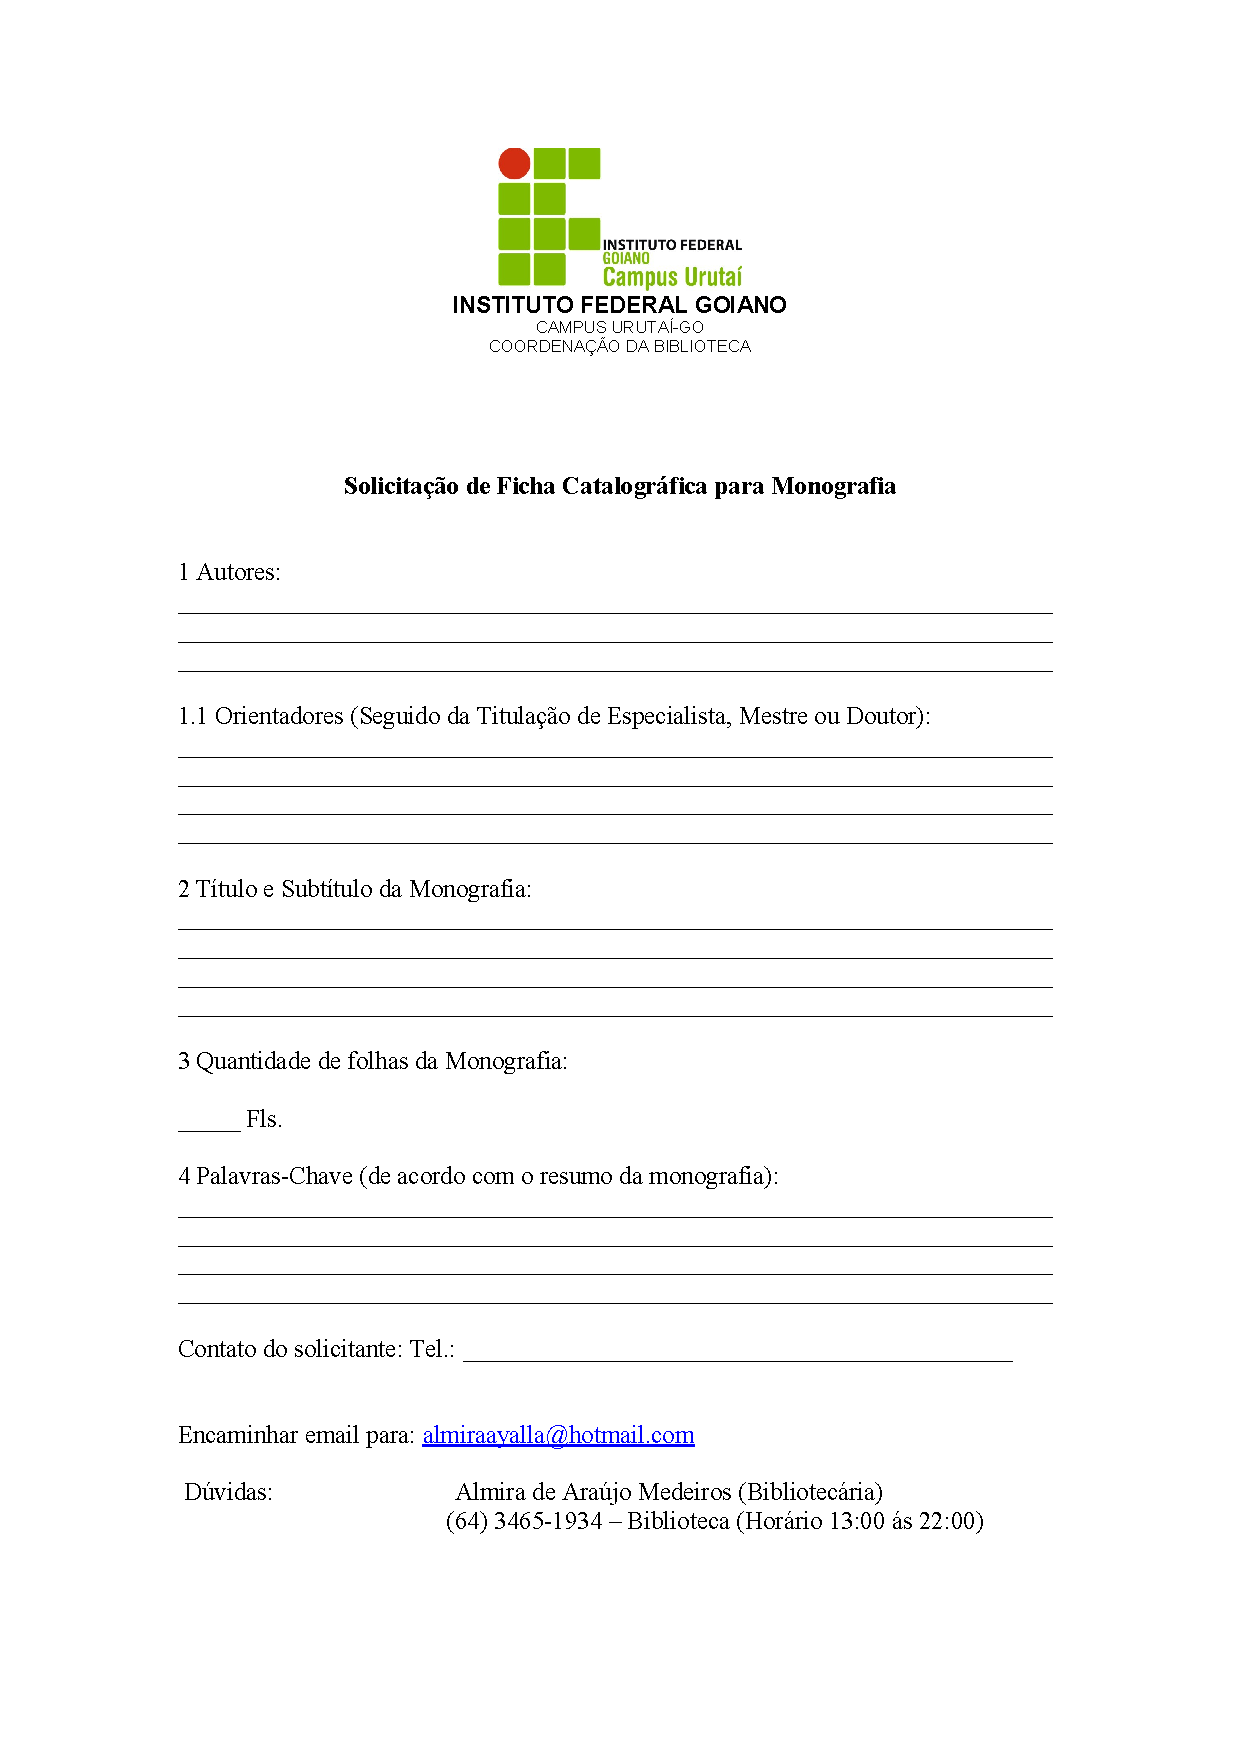
\includegraphics[scale=0.9]{figuras/solic_ficha_catalografica.pdf}
\end{figure}


Anexos devem conter informações e documentos que tenham sido confeccionados por terceiros e não pelo autor, ao contrário deste anexo, não é preciso inserir texto! Vale lembrar que não é estritamente necessário incluir anexos. 

Como exemplo este anexo traz o documento de solicitação de ficha catalográfica, a ser entregue na biblioteca, após a aprovação do trabalho em banca de defesa.
A versão final sem a ficha não será aceita, e a confecção da ficha antes da defesa também não, pois algumas informações só podem ser fornecidas após todas as correções.

\bigskip

\hspace{-2cm}

 
\end{document}